\write18{./make_talk.sh }

\documentclass[aspectratio=169]{beamer}
\usetheme{Pittsburgh}
\usecolortheme{spruce}
\usefonttheme{structurebold}
\beamertemplatenavigationsymbolsempty
\usepackage{graphicx}
\usepackage{tikz}
\usepackage{cite}
\usepackage{pgfpages}
\usepackage{bm}

%% \setbeameroption{hide notes}
\input{.mk.out}

\title{Far Flung Forest Landscapes in the Anthropocene}
\subtitle{Structural analysis of China's embodied forest network}
\author{Matthew Kekoa Lau (Ph.D.) \\ Yu Liang, Bo Liu}
\date{}
\institute{Chinese Academy of Sciences and Harvard University \\
                    \\
                   Email: mk@mklau.info \\
                   Website: \url{https://people.fas.harvard.edu/~matthewklau} \\
                   ResearchGate: \url{Matthew_Lau2}}


\begin{document}

{
\usebackgroundtemplate{
\begin{tikzpicture}[remember picture,overlay]
        \node[at=(current page.center), opacity=0.40]{
                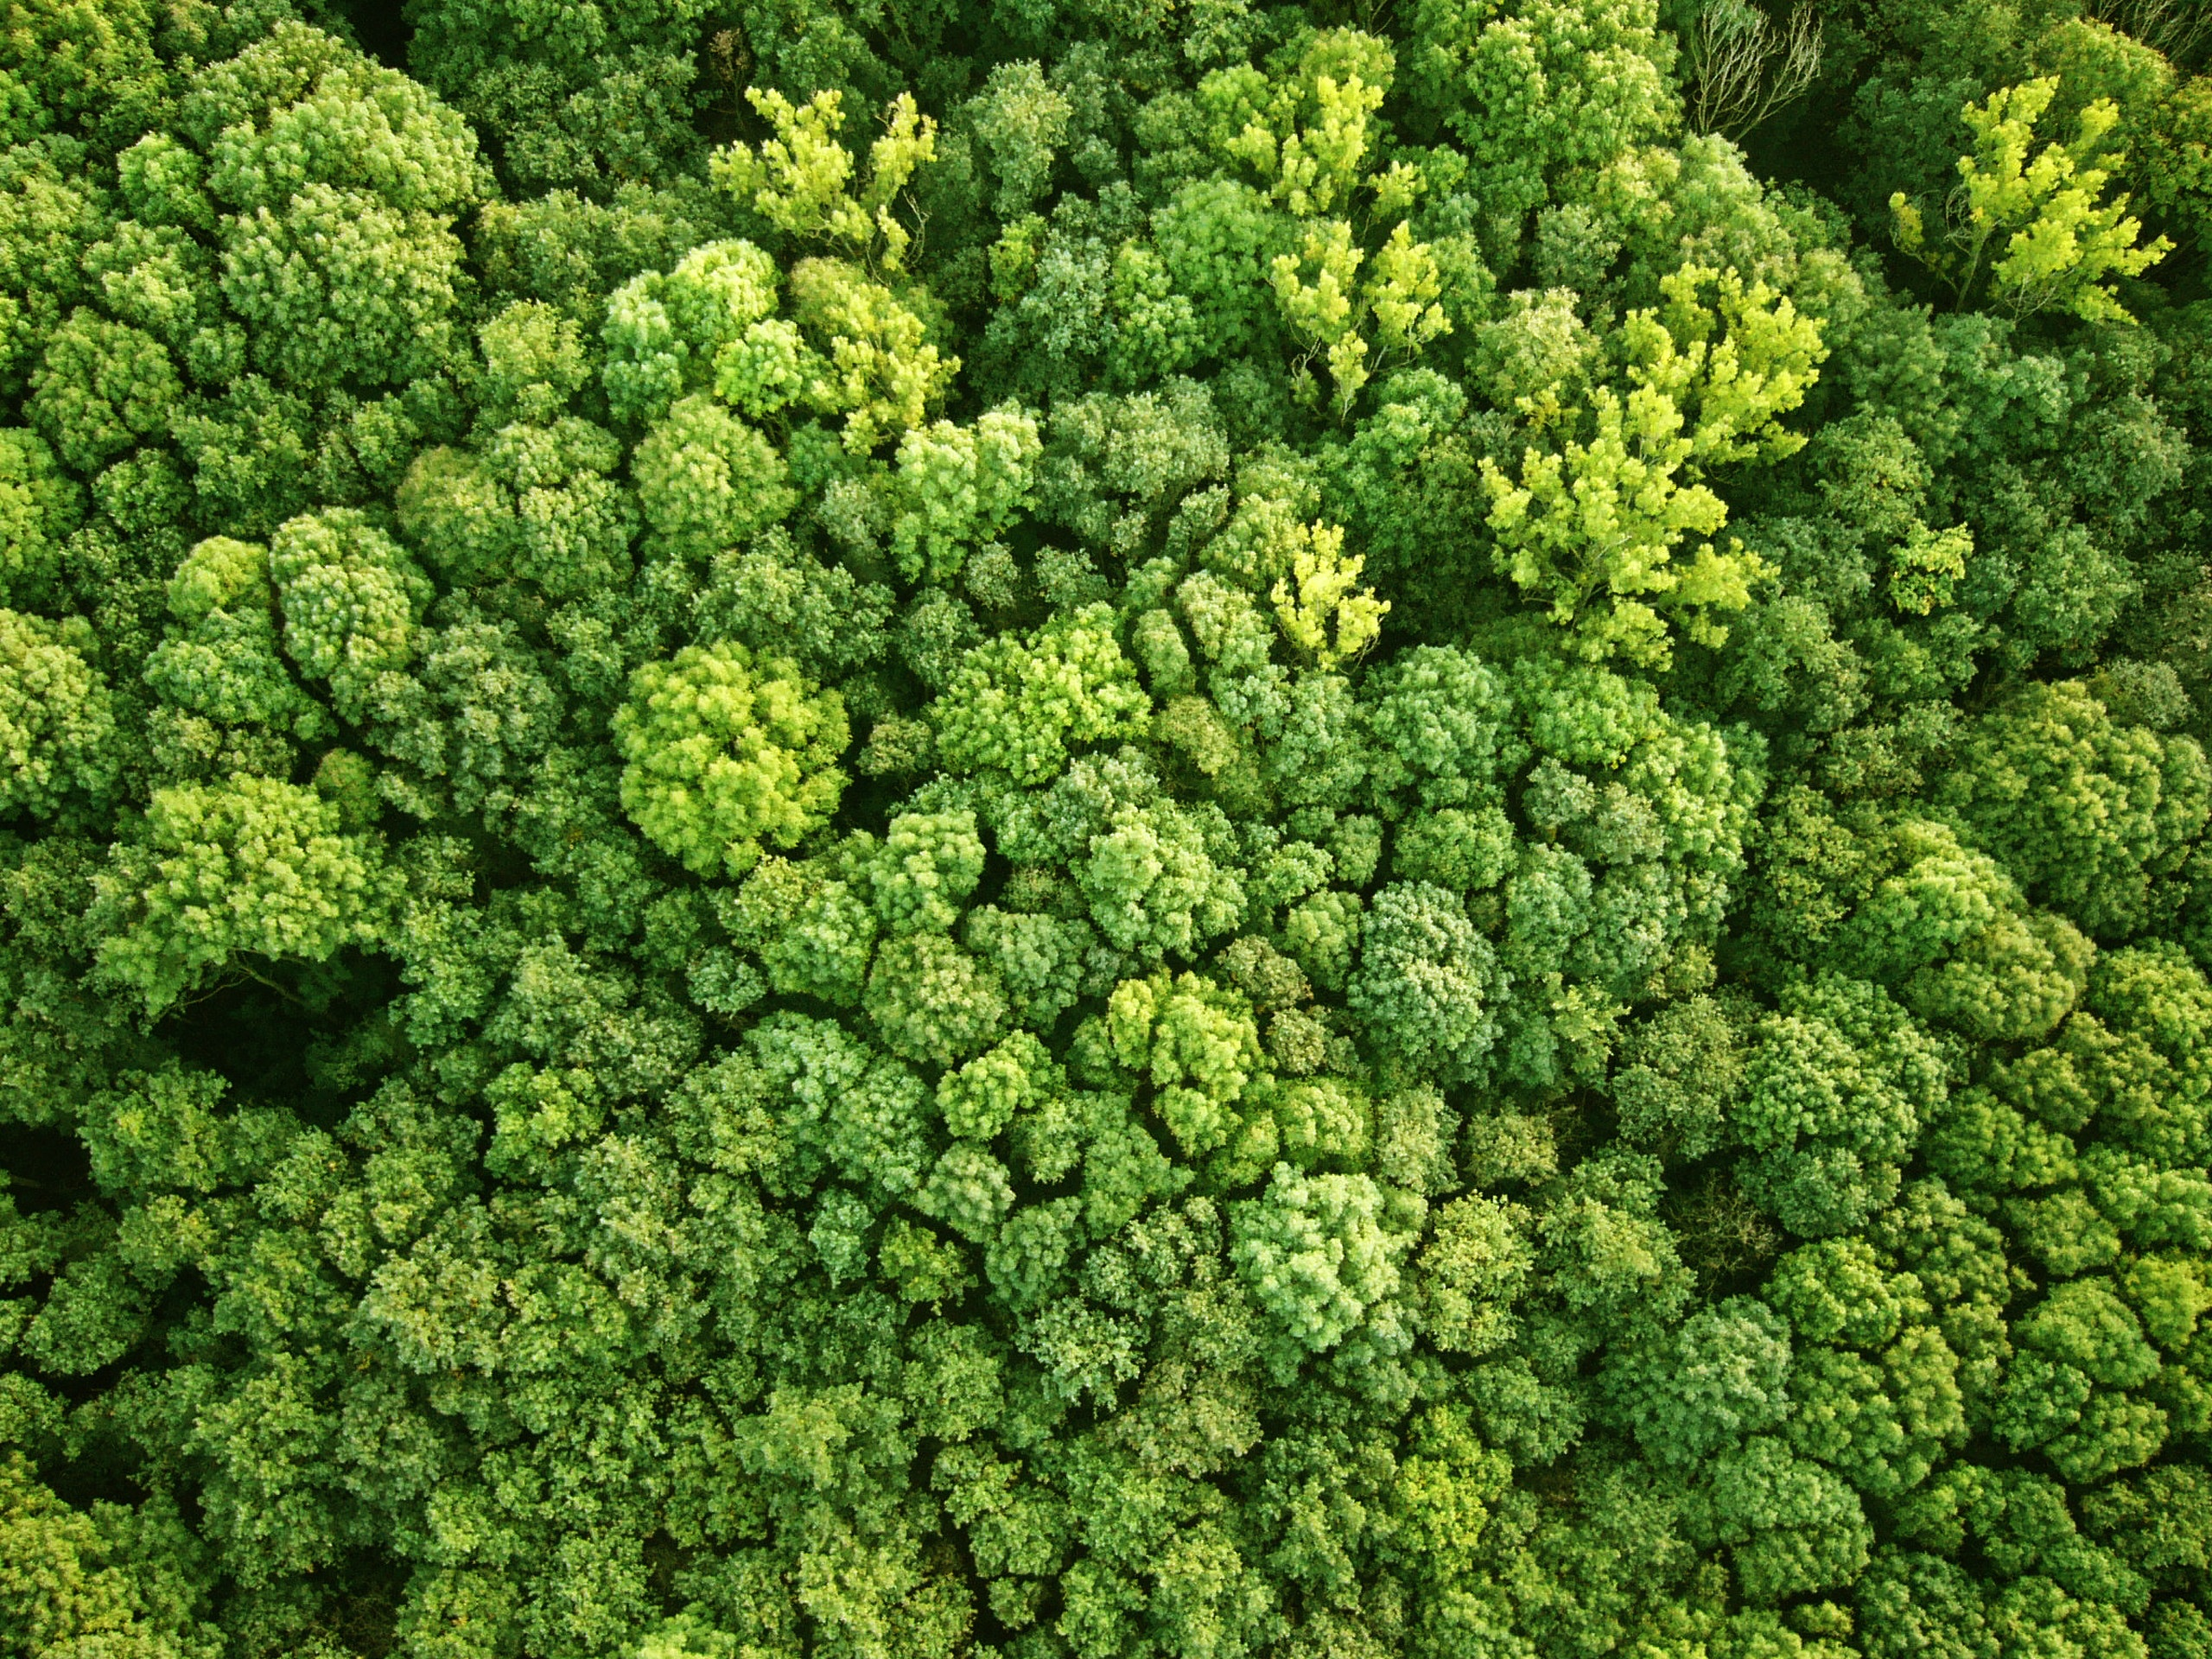
\includegraphics[keepaspectractio, width=\paperwidth]{images/forest_aerial.jpg}
        };
\end{tikzpicture}
}
\begin{frame}
  \titlepage
  \note[item]{Thanks to Dave Smith and anyone else who's helped to
  organize this seminar, it's a pleasure for me to speak about my
  recent work}
  \note[item]{Forests $\sim$ 80\% terrestrial biodiversity (WWF)}
  \note[item]{Soil stabilization}
  \note[item]{Forests carry out important processes: clean air and water}
  \note[item]{Forests store carbon}
\end{frame}
}

\section*{Context}

{ % all template changes are local to this group.
%%    \setbeamertemplate{navigation symbols}{}
    \begin{frame}<article:0>[plain]
      \frametitle{}
        \begin{tikzpicture}[remember picture,overlay]
            \node[at=(current page.center)] {
                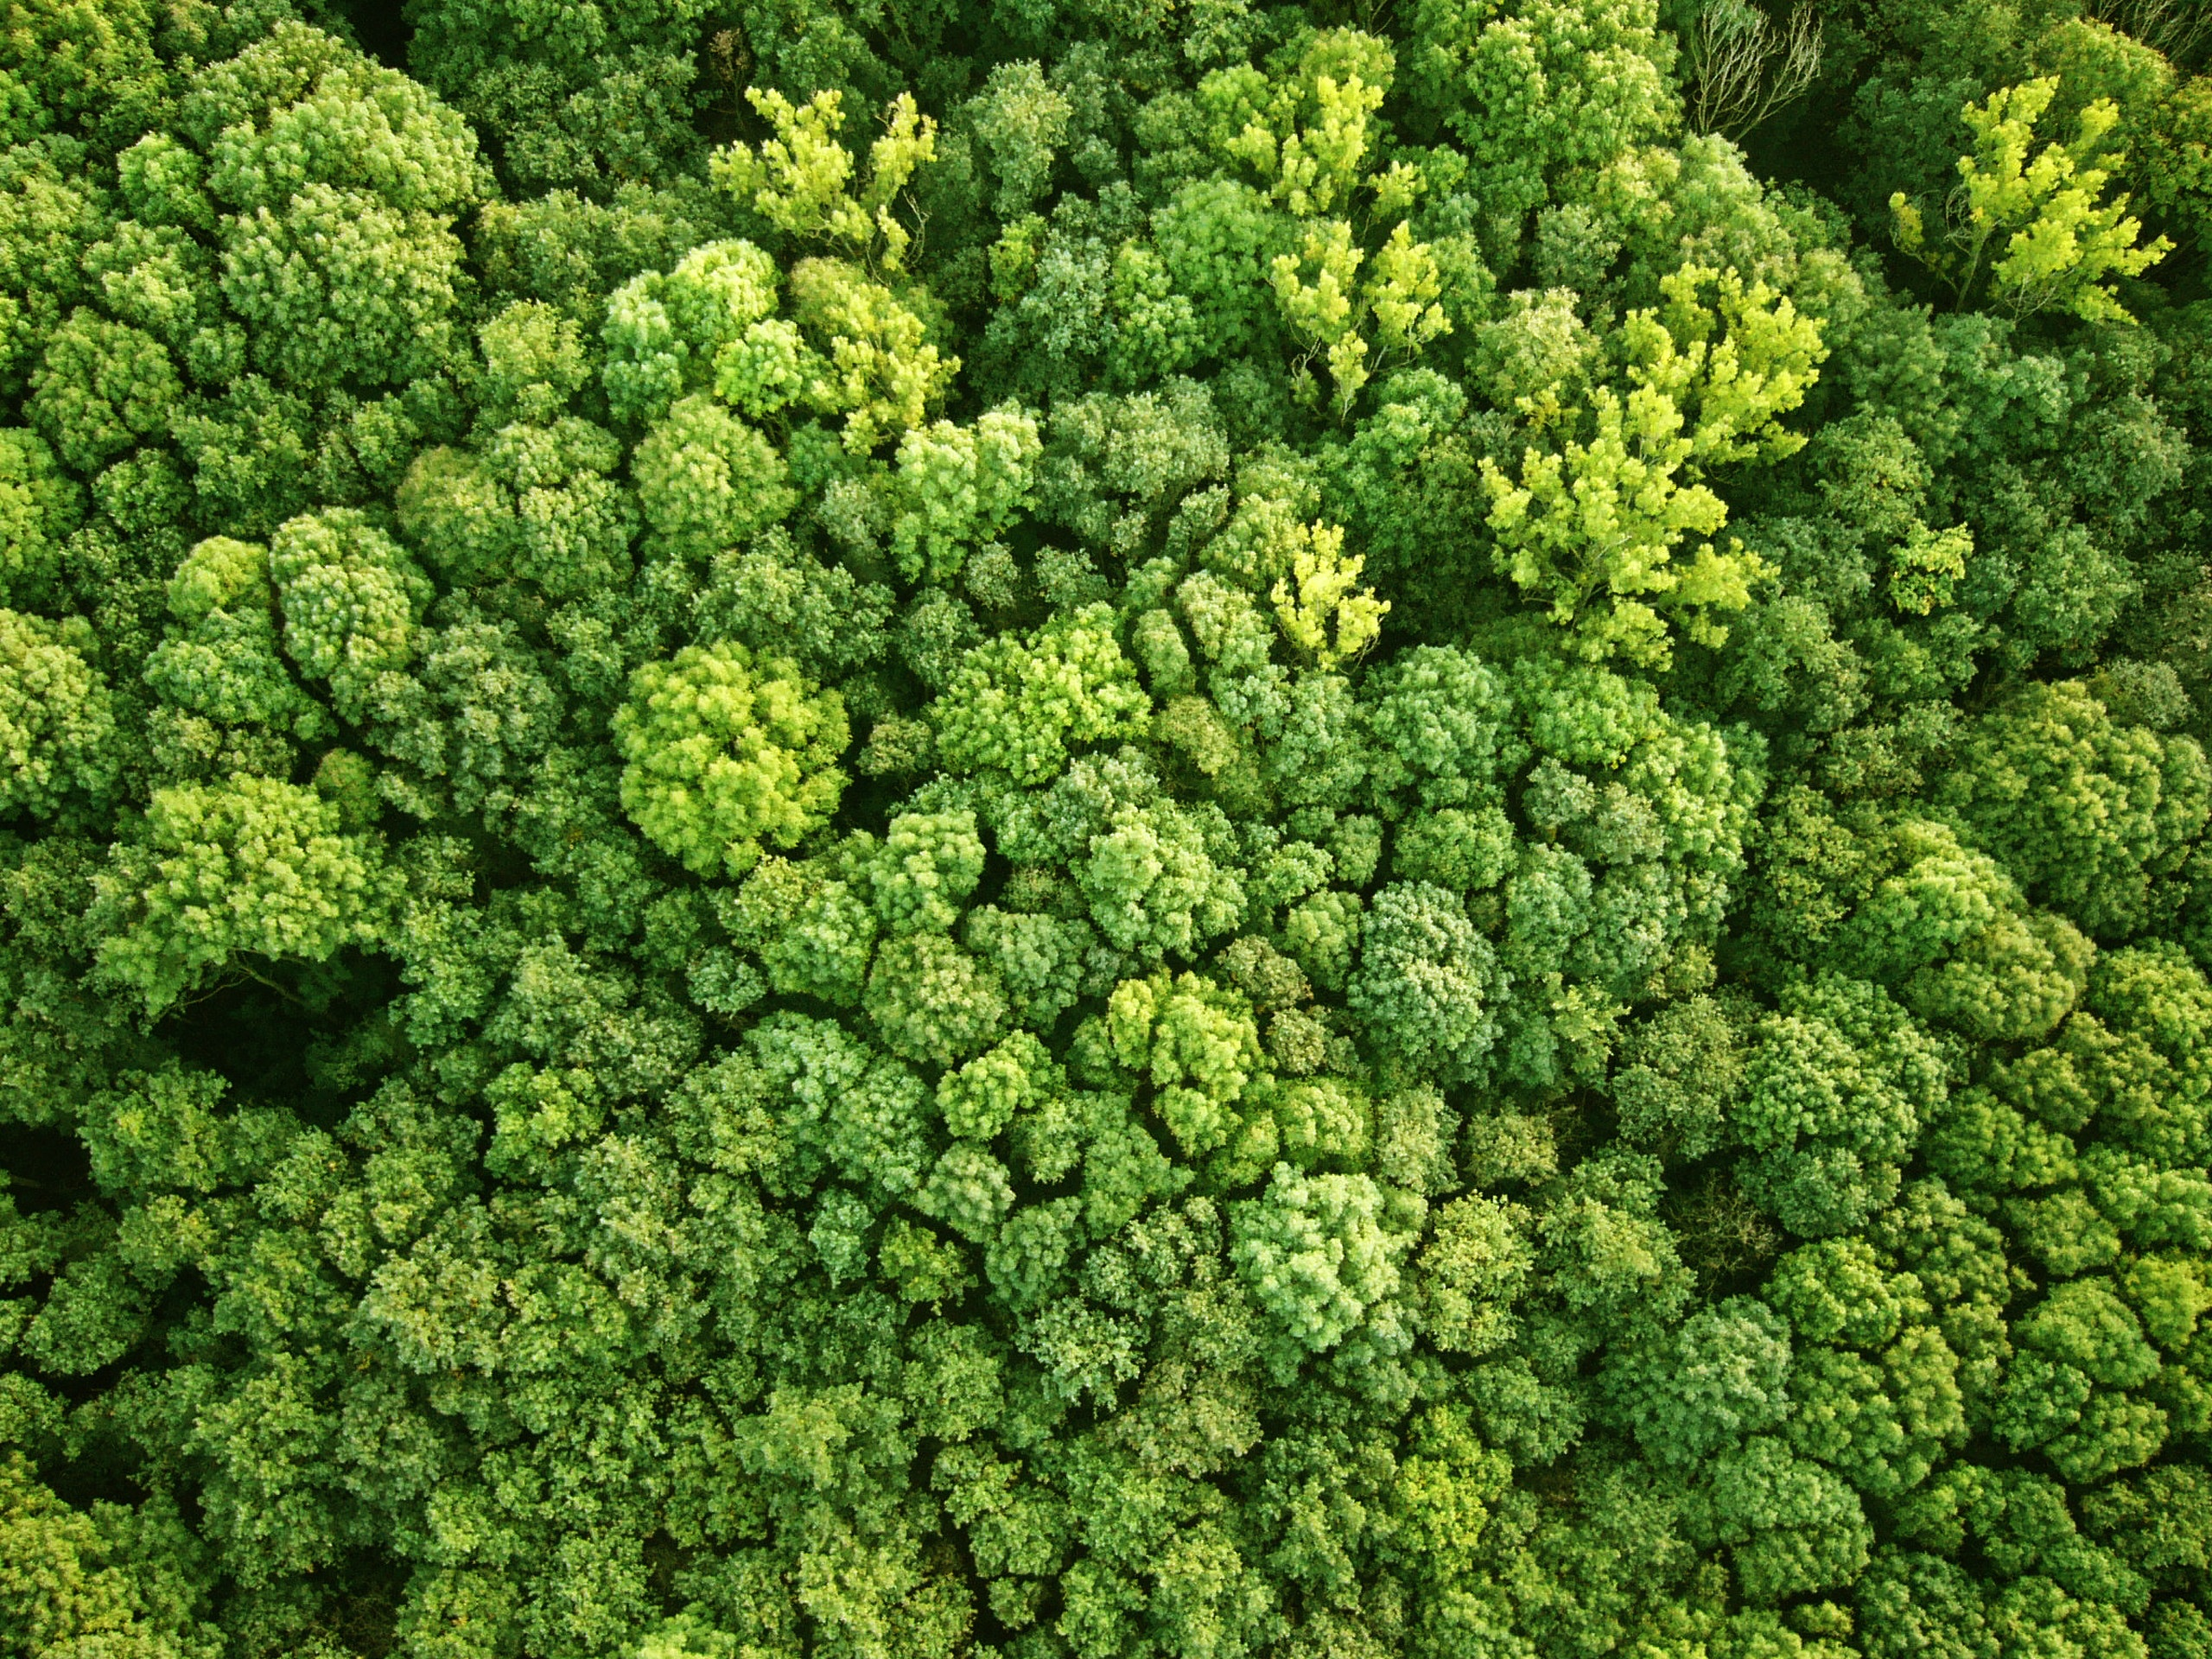
\includegraphics[keepaspectratio,
                                 width=\paperwidth]{images/forest_aerial.jpg}
            };
        \end{tikzpicture}
     \end{frame}
}

{ % all template changes are local to this group.
%%    \setbeamertemplate{navigation symbols}{}
    \begin{frame}<article:0>[plain]
      \frametitle{}
        \begin{tikzpicture}[remember picture,overlay]
            \node[at=(current page.center)] {
                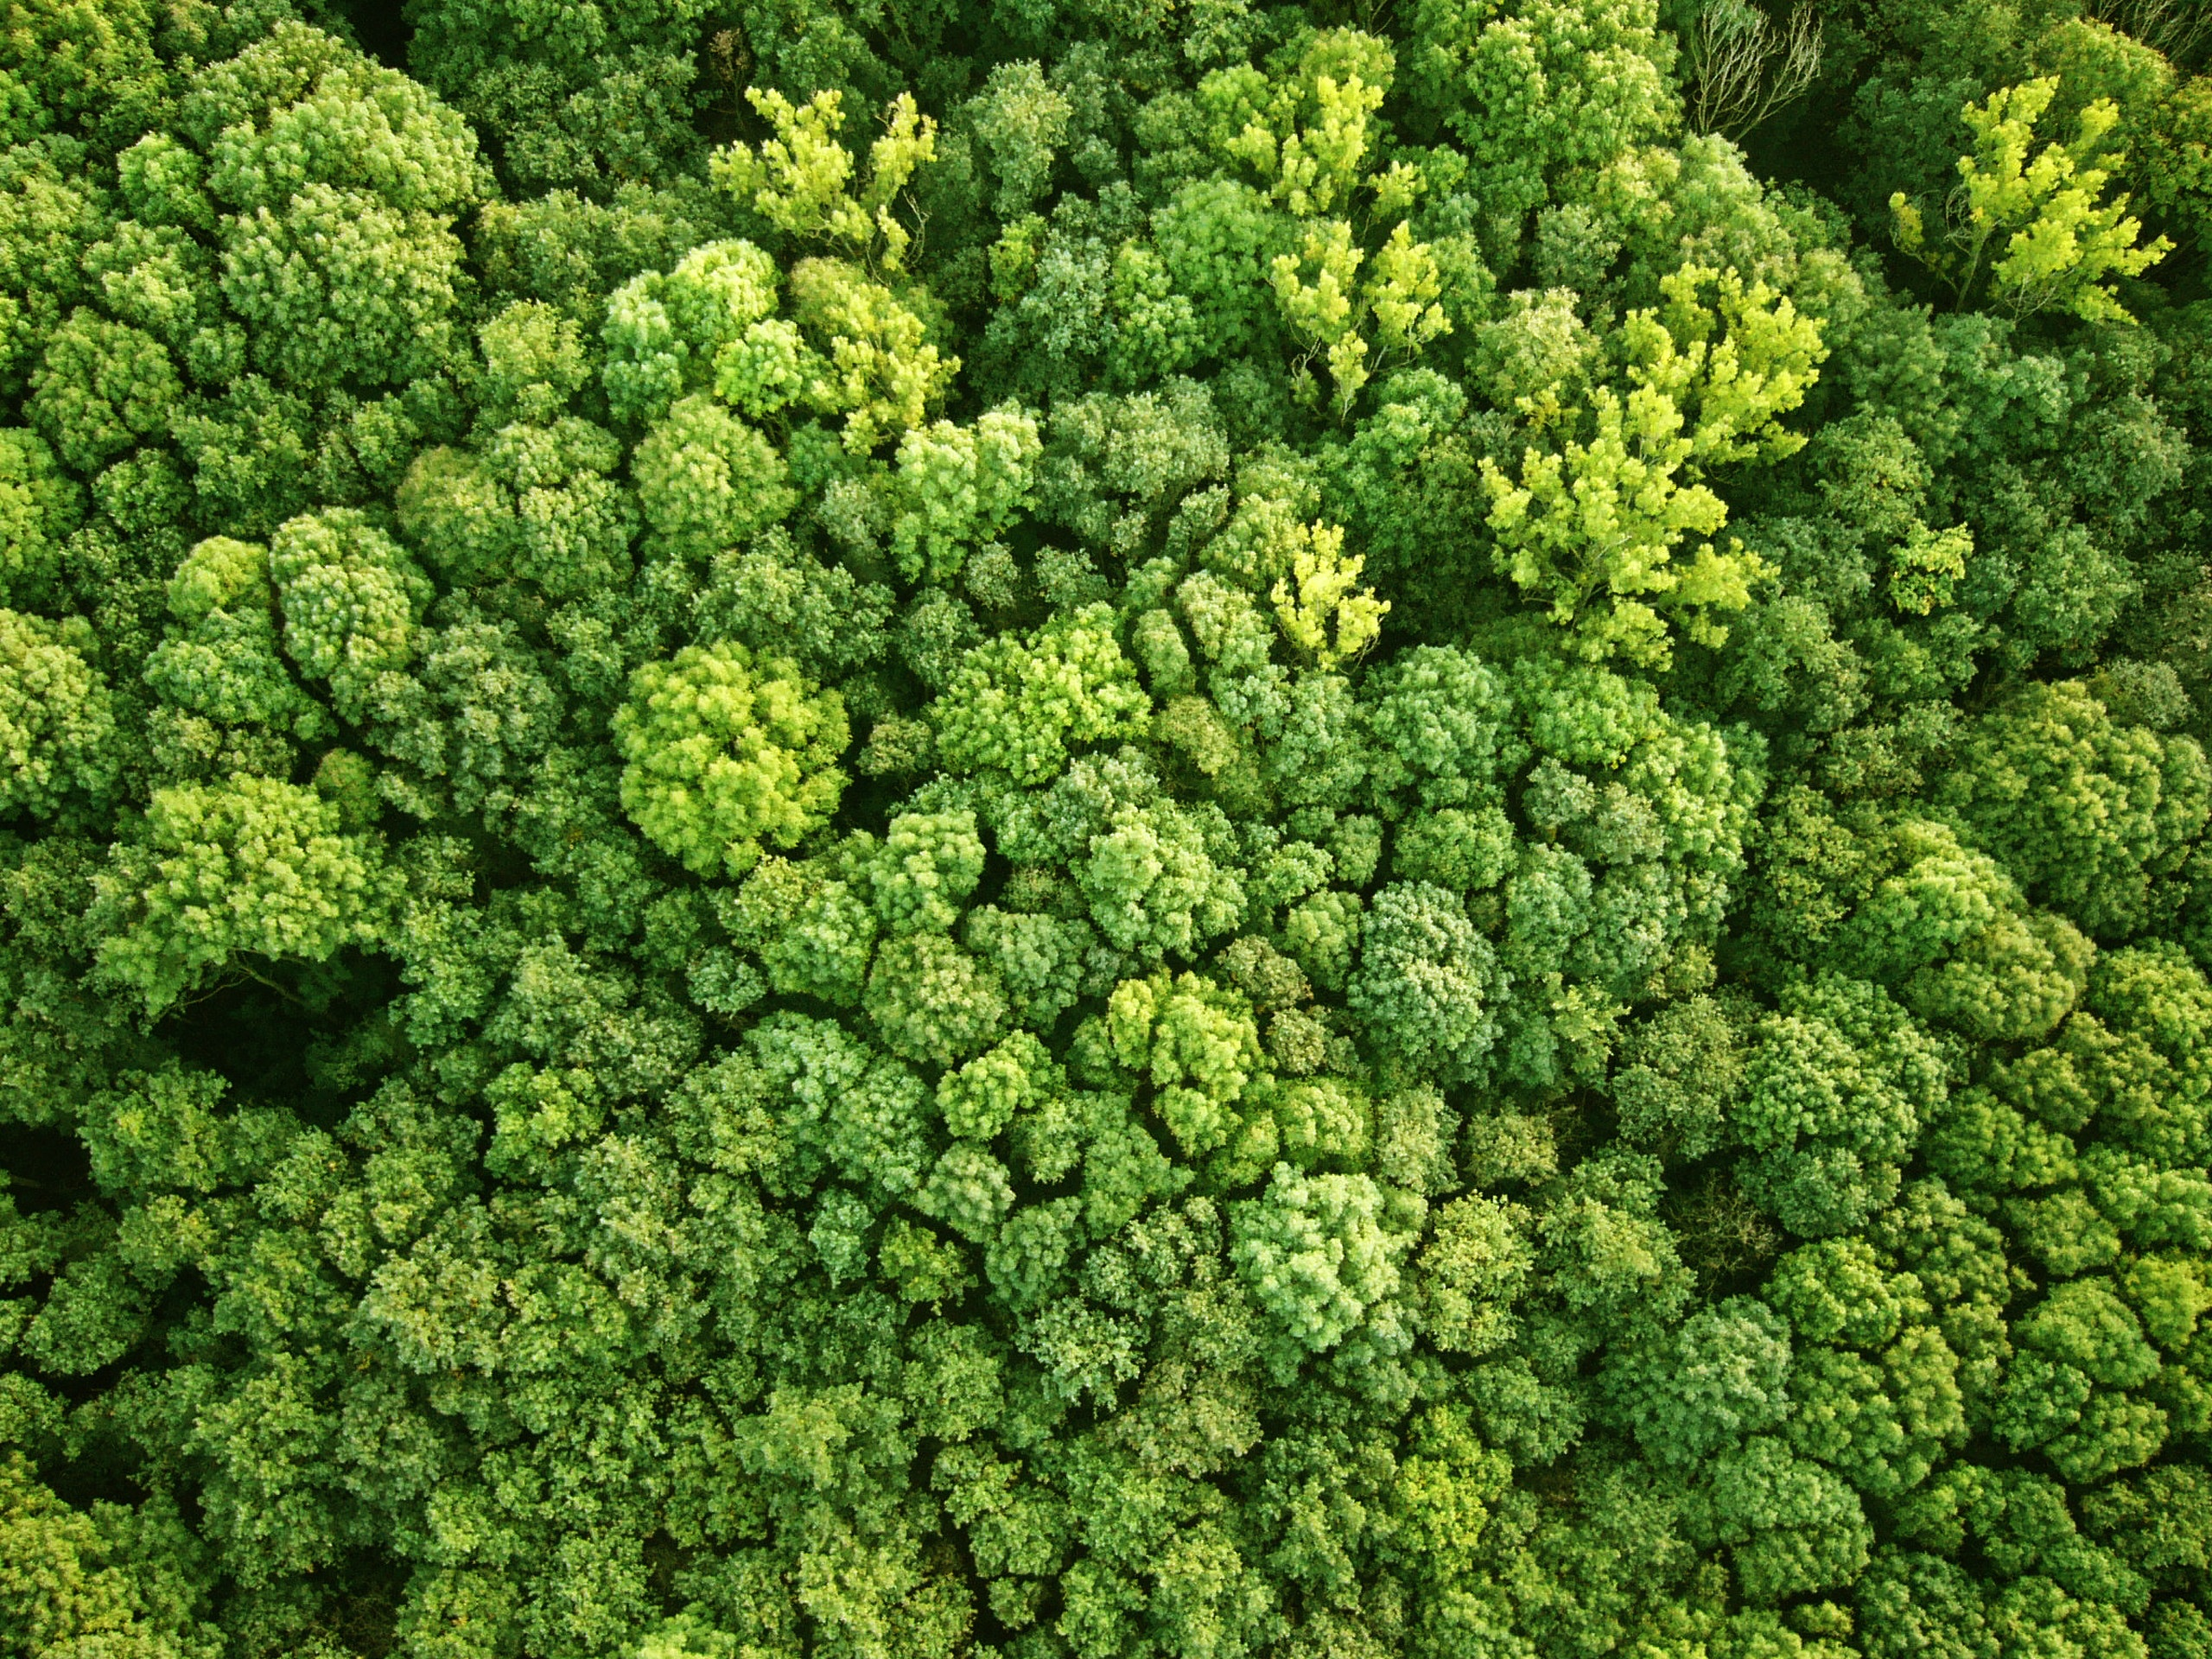
\includegraphics[keepaspectratio,
                                 width=\paperwidth]{images/forest_aerial.jpg}
            };
            \node[at=(current page.center)] {
                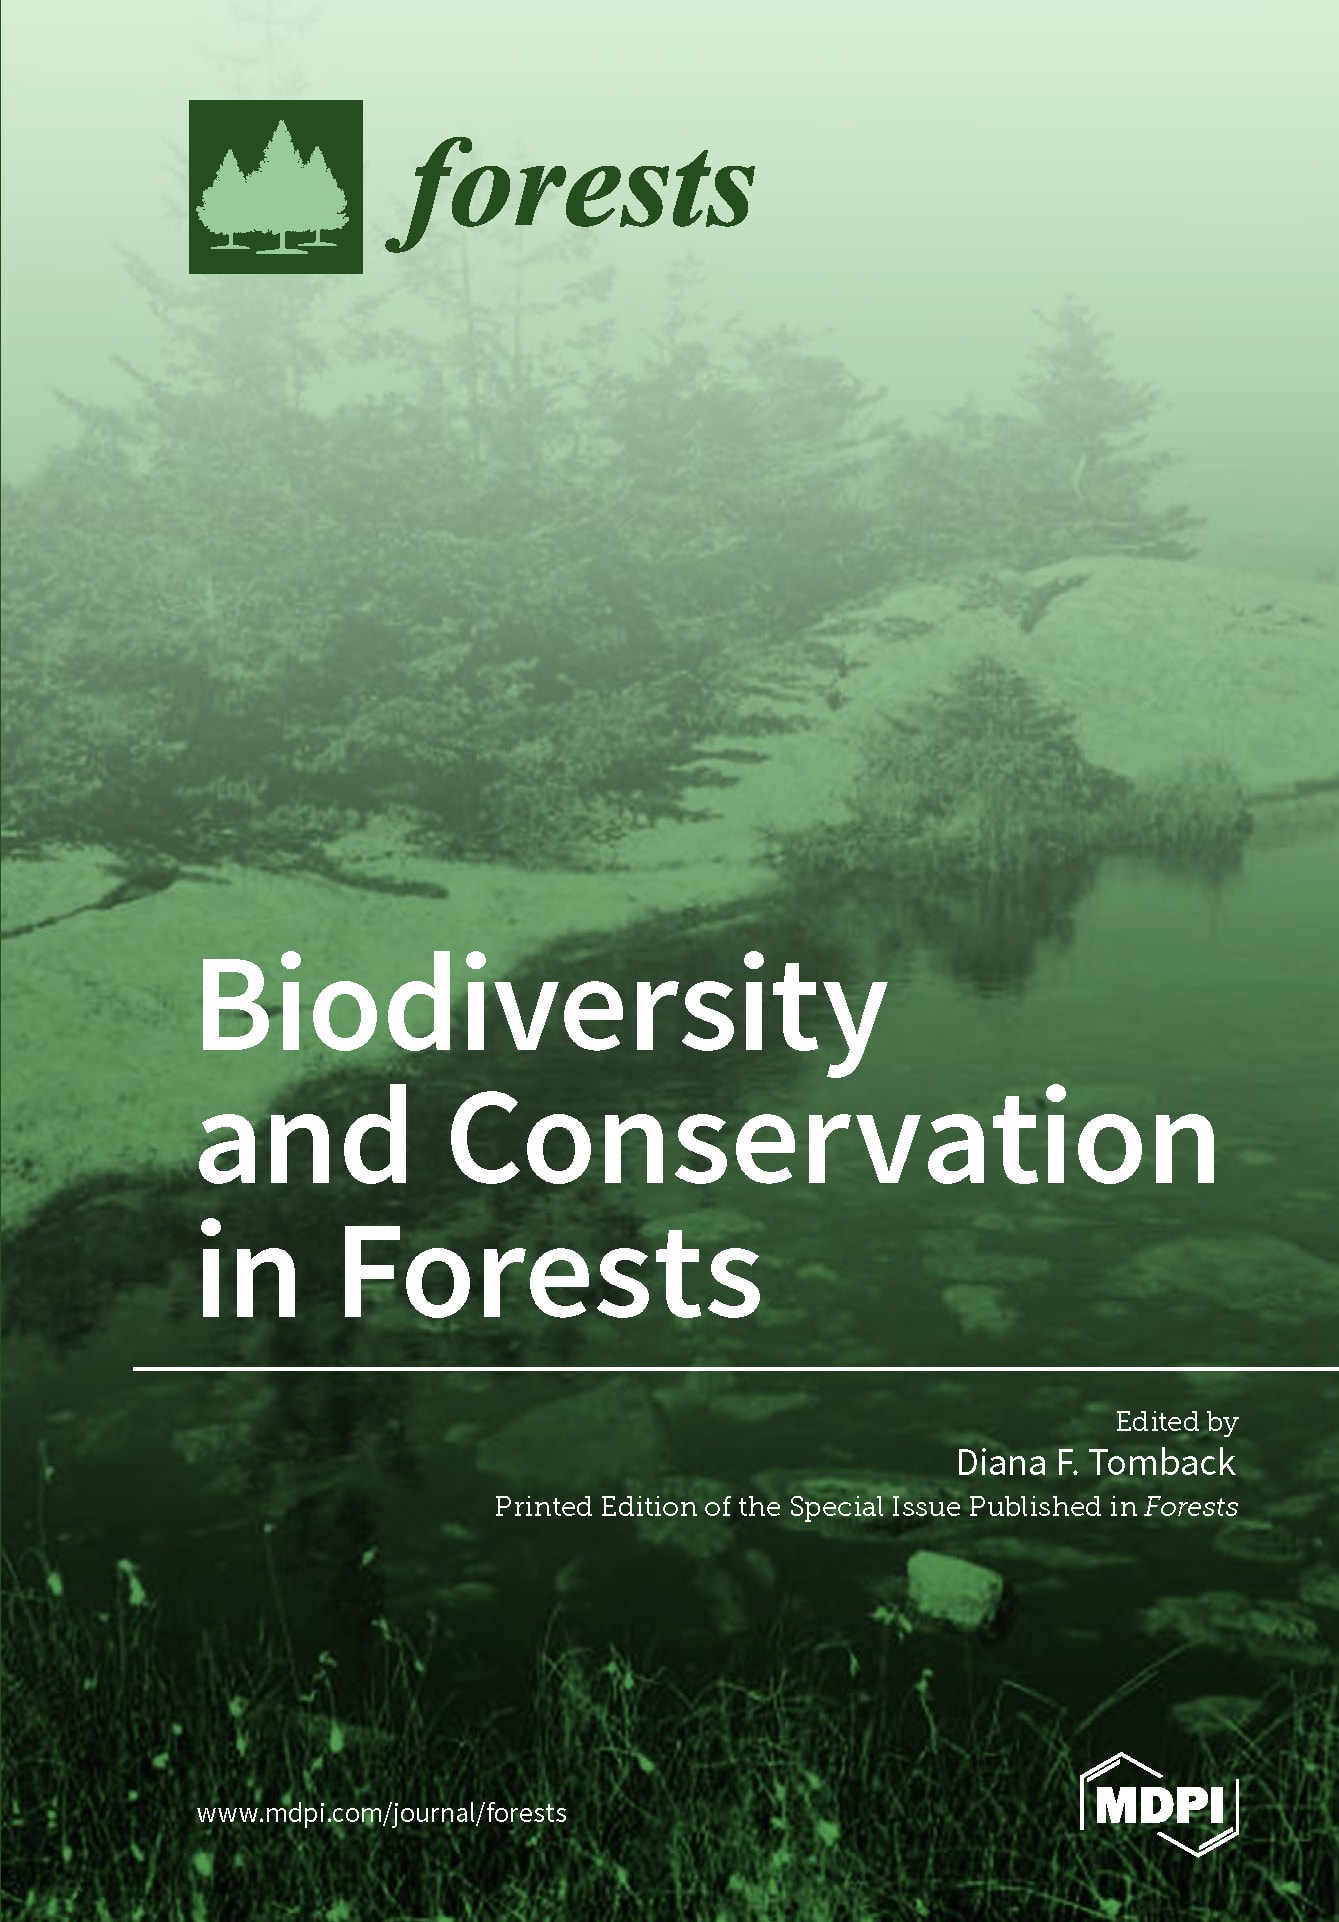
\includegraphics[keepaspectratio,
                                 height=\paperheight]{images/forest_biodiversity.jpg}
            };
        \end{tikzpicture}
     \end{frame}
}

{ % all template changes are local to this group.
%%    \setbeamertemplate{navigation symbols}{}
    \begin{frame}<article:0>[plain]
      \frametitle{}
        \begin{tikzpicture}[remember picture,overlay]
            \node[at=(current page.center)] {
                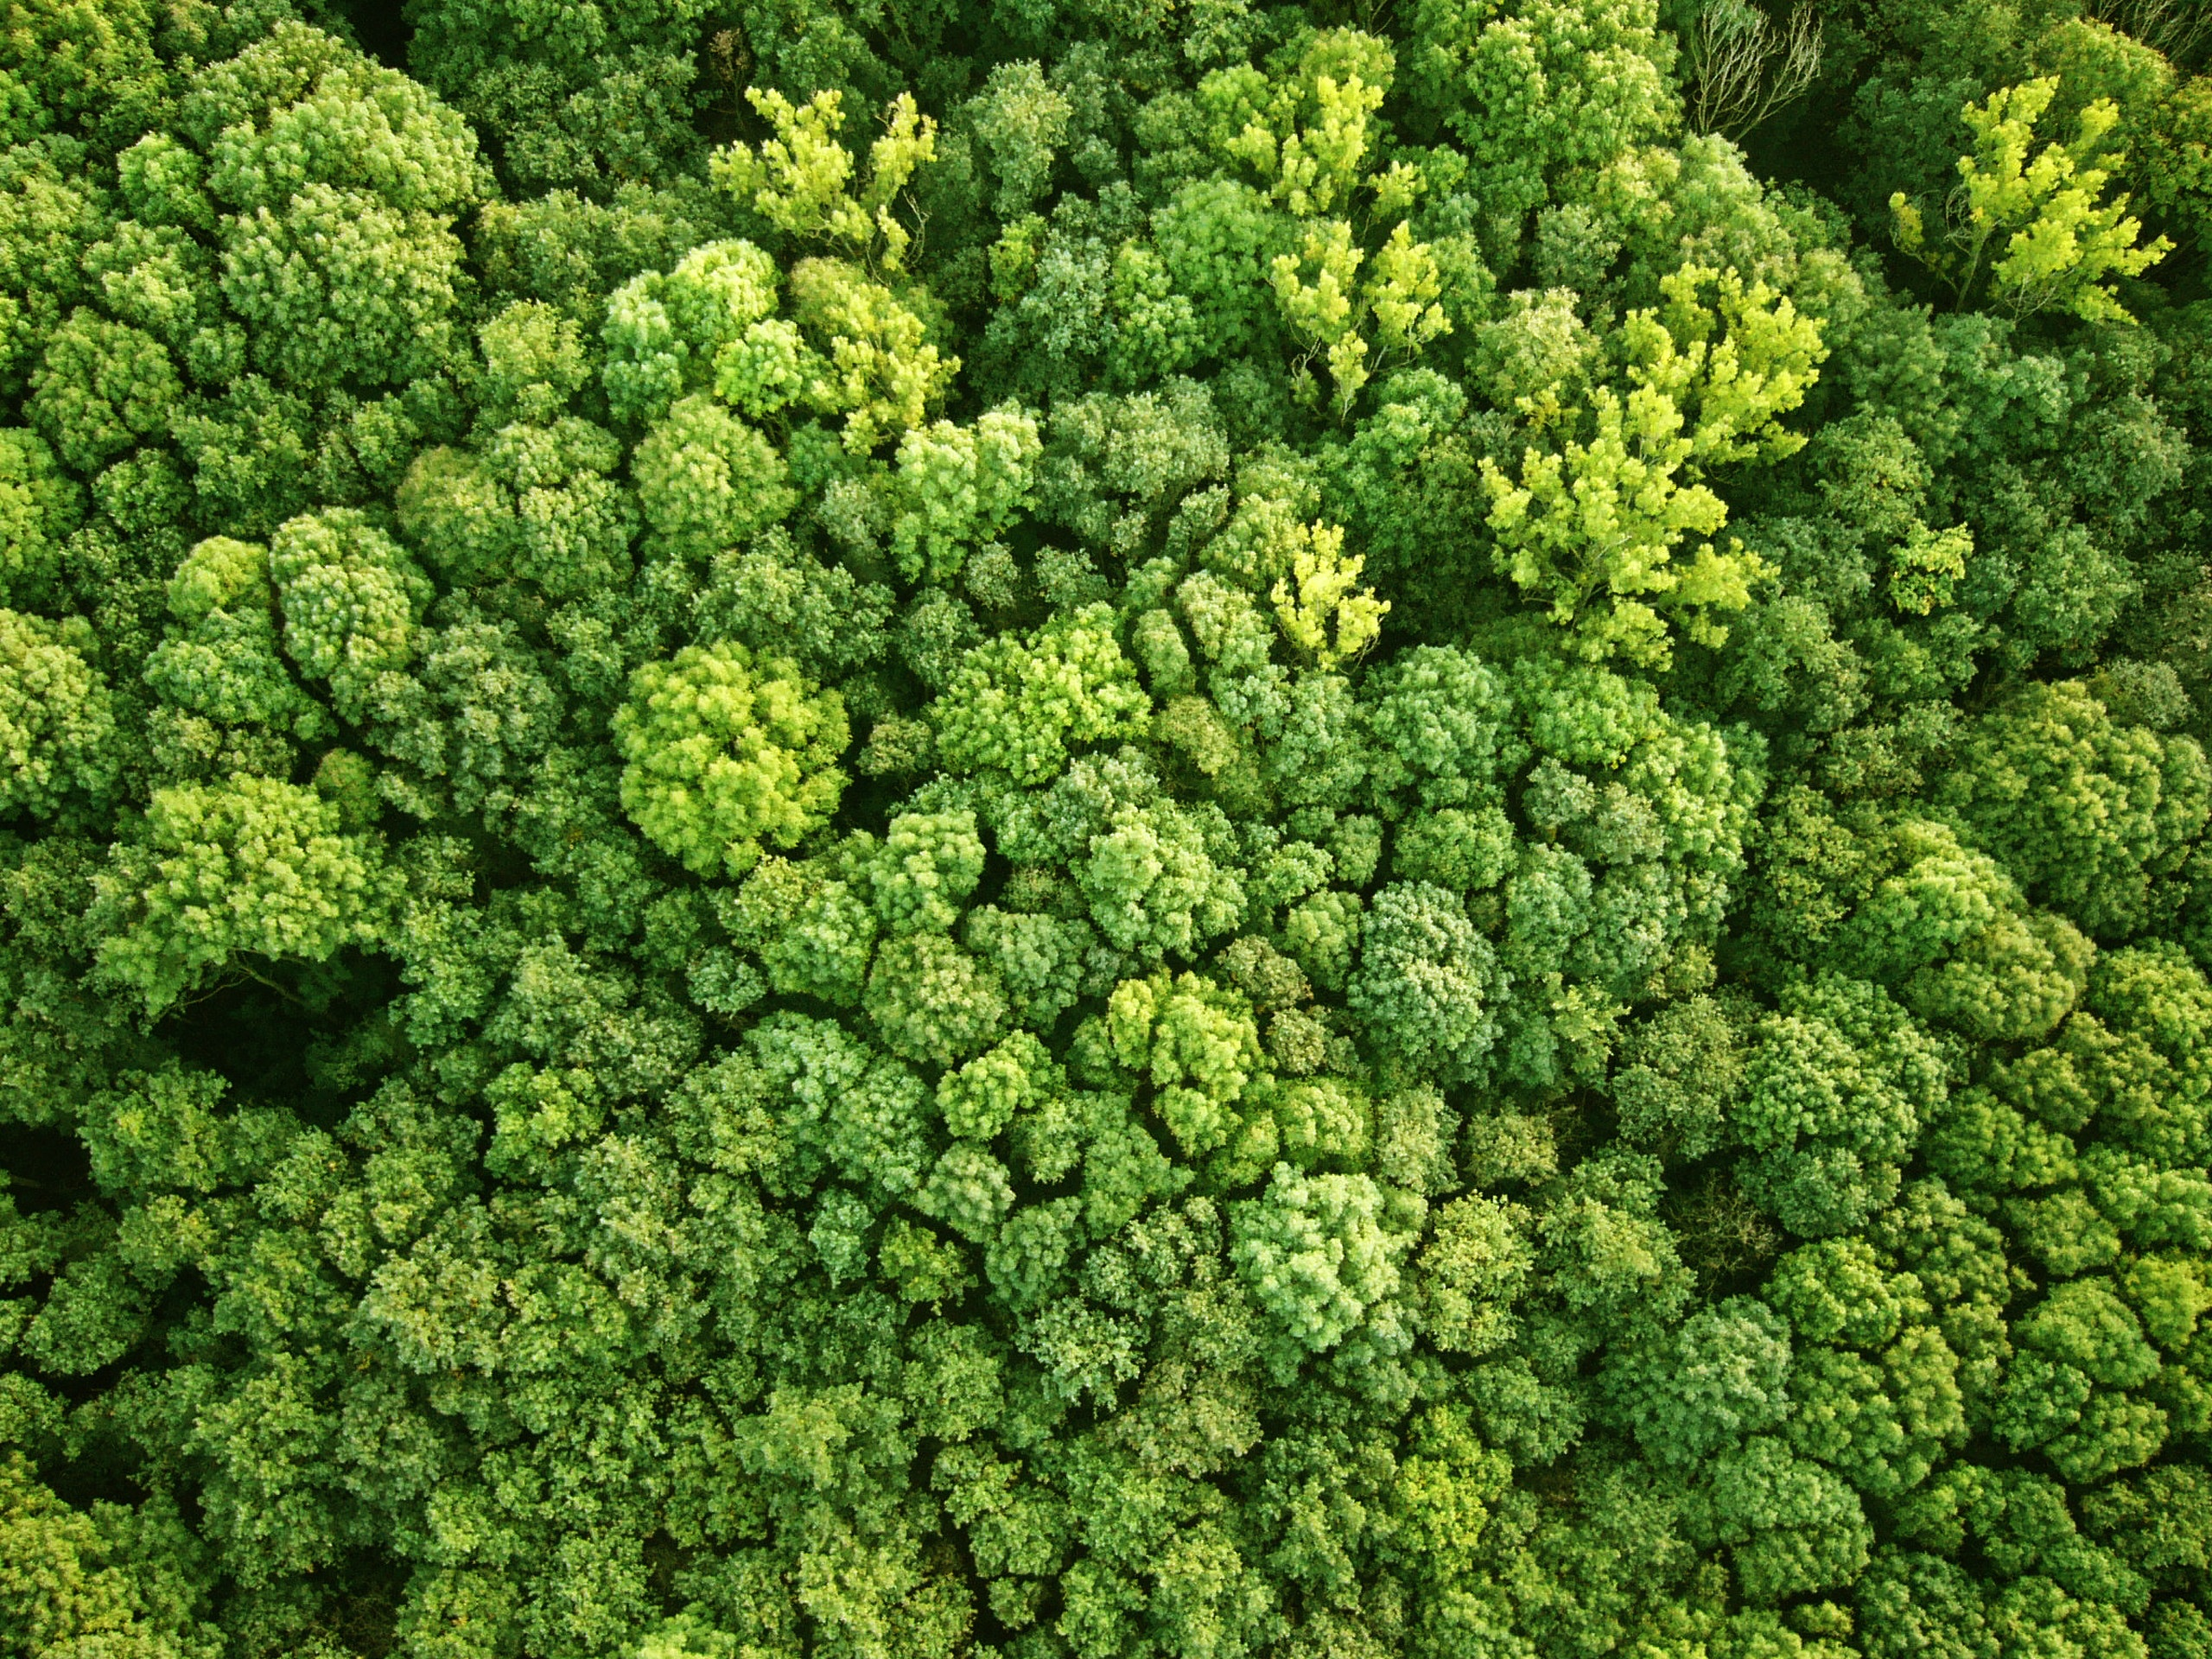
\includegraphics[keepaspectratio,
                                 width=\paperwidth]{images/forest_aerial.jpg}
            };
            \node[at=(current page.center)] {
                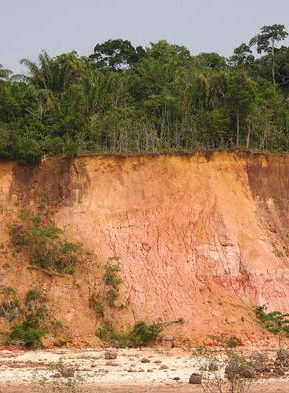
\includegraphics[keepaspectratio,
                                 height=\paperheight]{images/soil_sability.jpg}
            };
        \end{tikzpicture}
     \end{frame}
}


{ % all template changes are local to this group.
%%    \setbeamertemplate{navigation symbols}{}
    \begin{frame}<article:0>[plain]
      \frametitle{}
        \begin{tikzpicture}[remember picture,overlay]
            \node[at=(current page.center)] {
                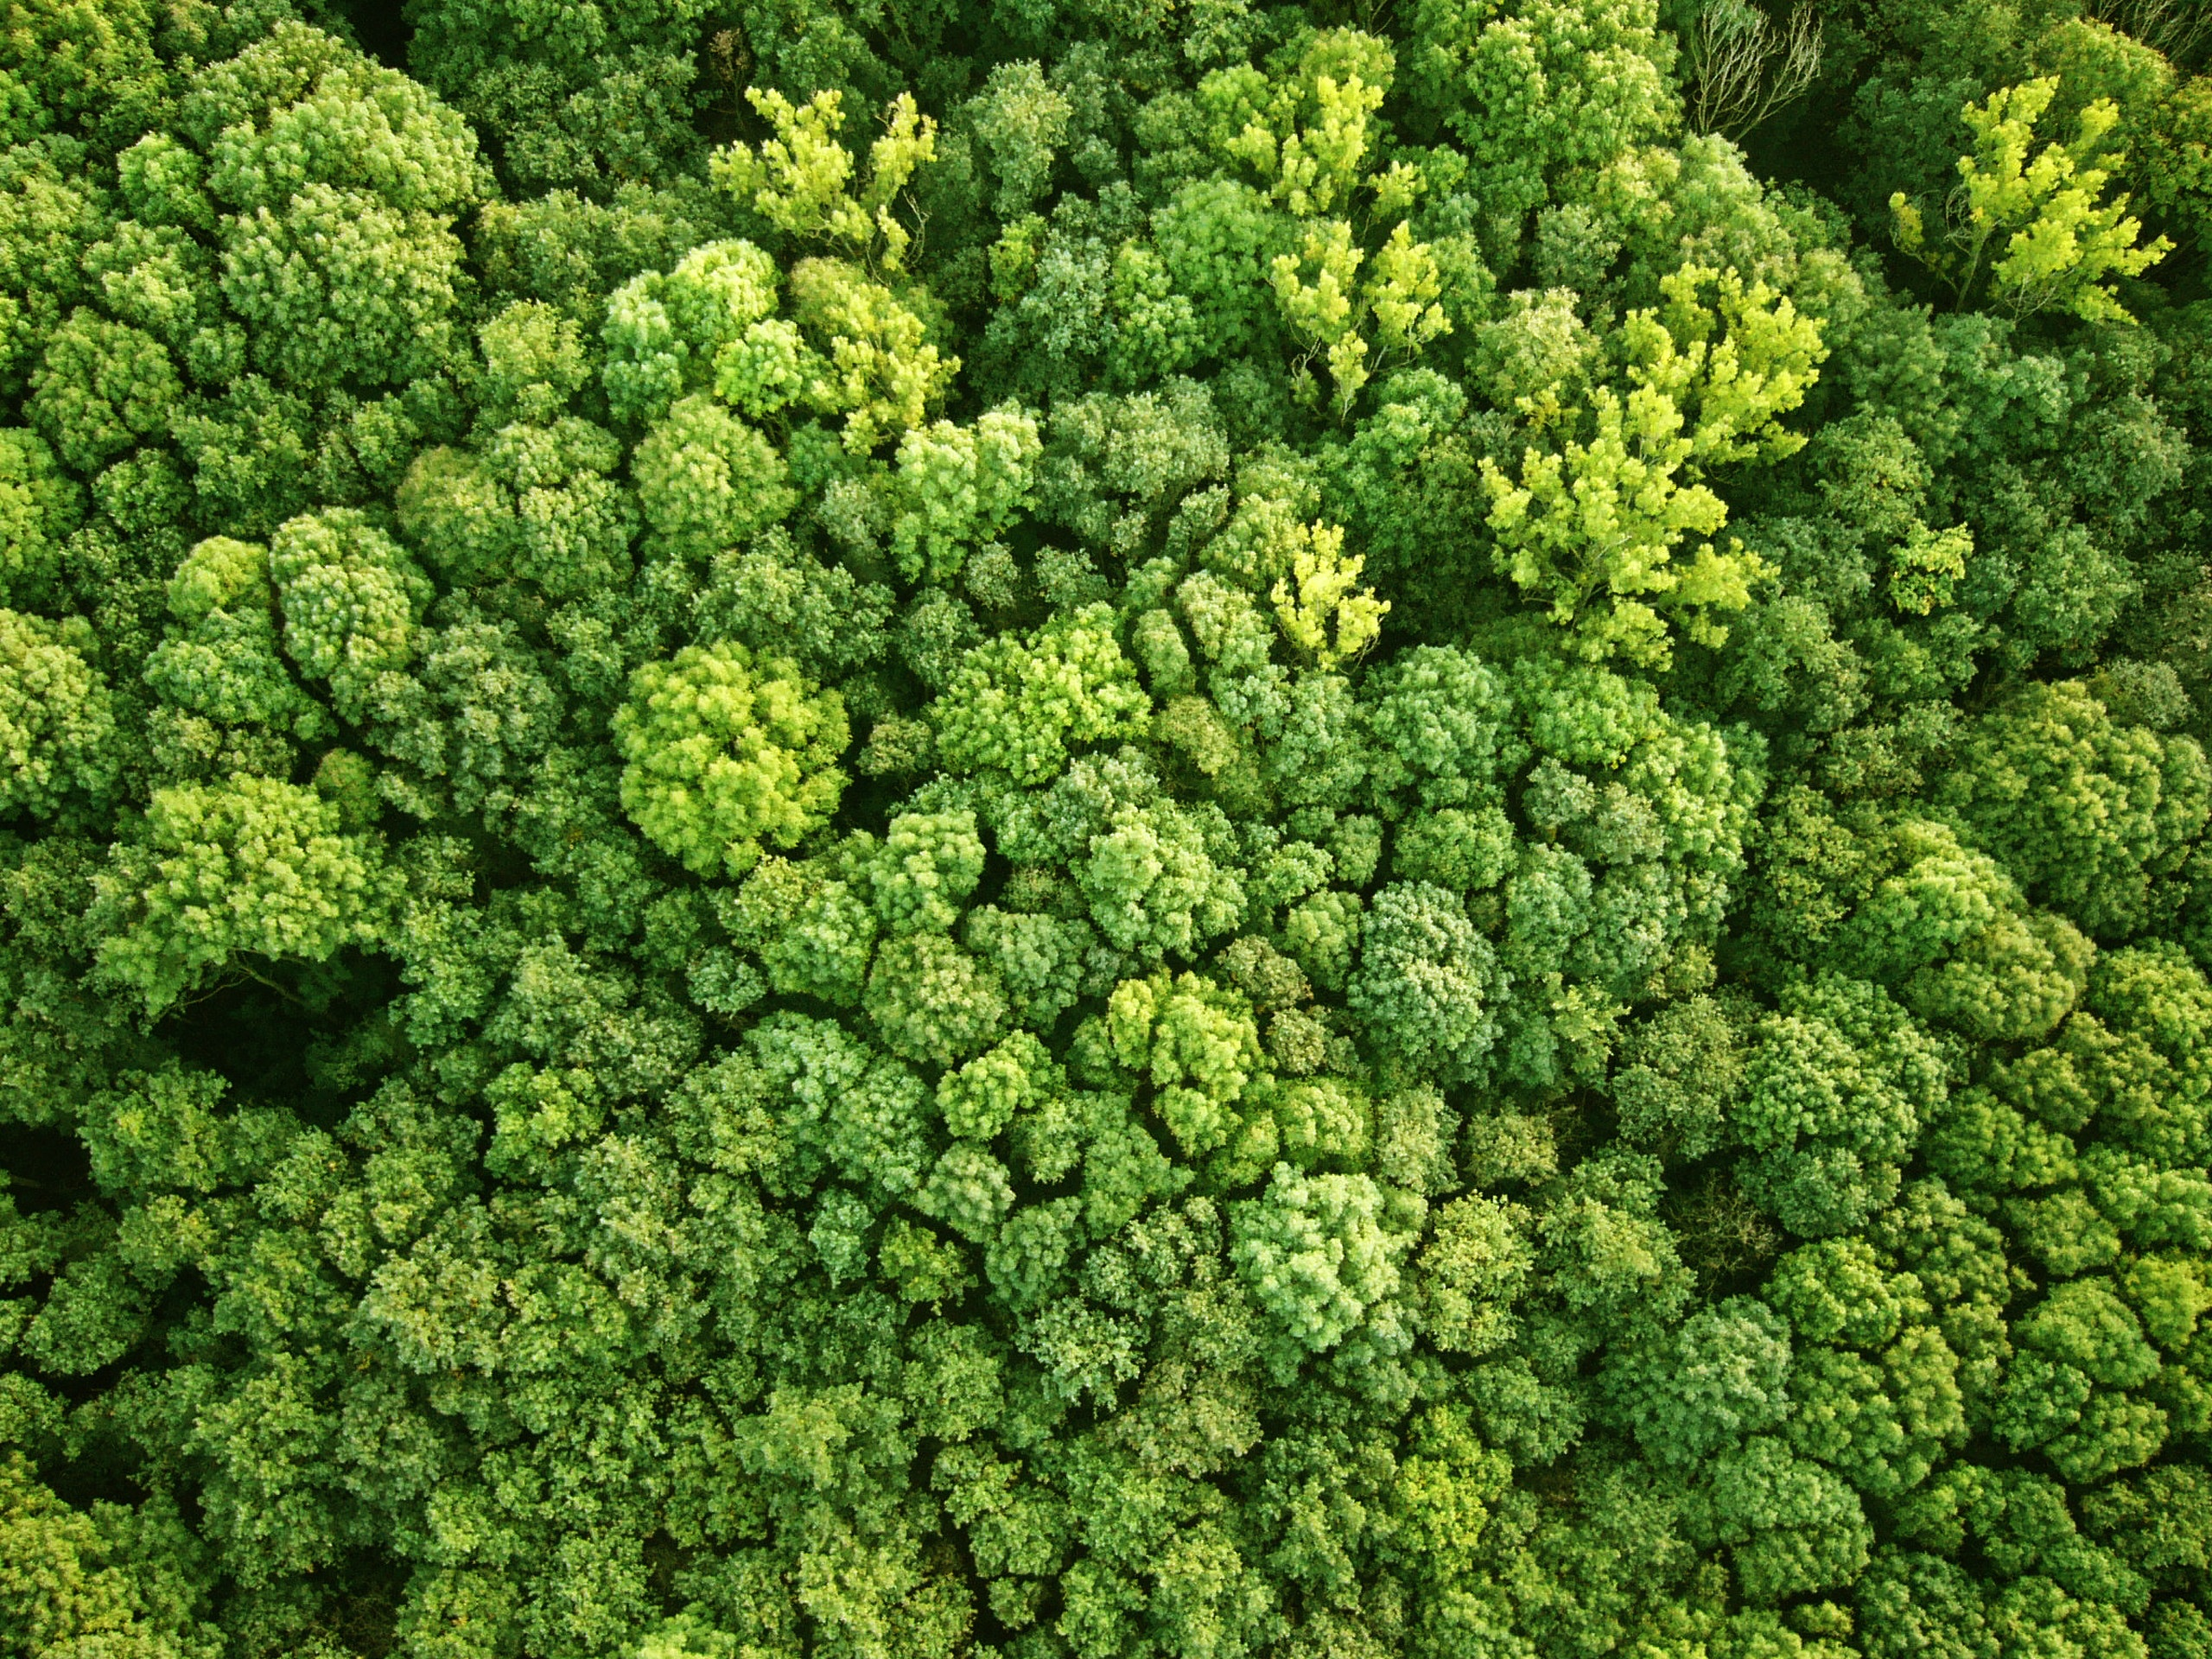
\includegraphics[keepaspectratio,
                                 width=\paperwidth]{images/forest_aerial.jpg}
            };
            \node[at=(current page.center)] {
                
\includegraphics[keepaspectratio,
                                 height=\paperheight]{images/glass-of-water.jpg}
            };
        \end{tikzpicture}
     \end{frame}
}


{ % all template changes are local to this group.
%%    \setbeamertemplate{navigation symbols}{}
    \begin{frame}<article:0>[plain]
      \frametitle{}
        \begin{tikzpicture}[remember picture,overlay]
            \node[at=(current page.center)] {
                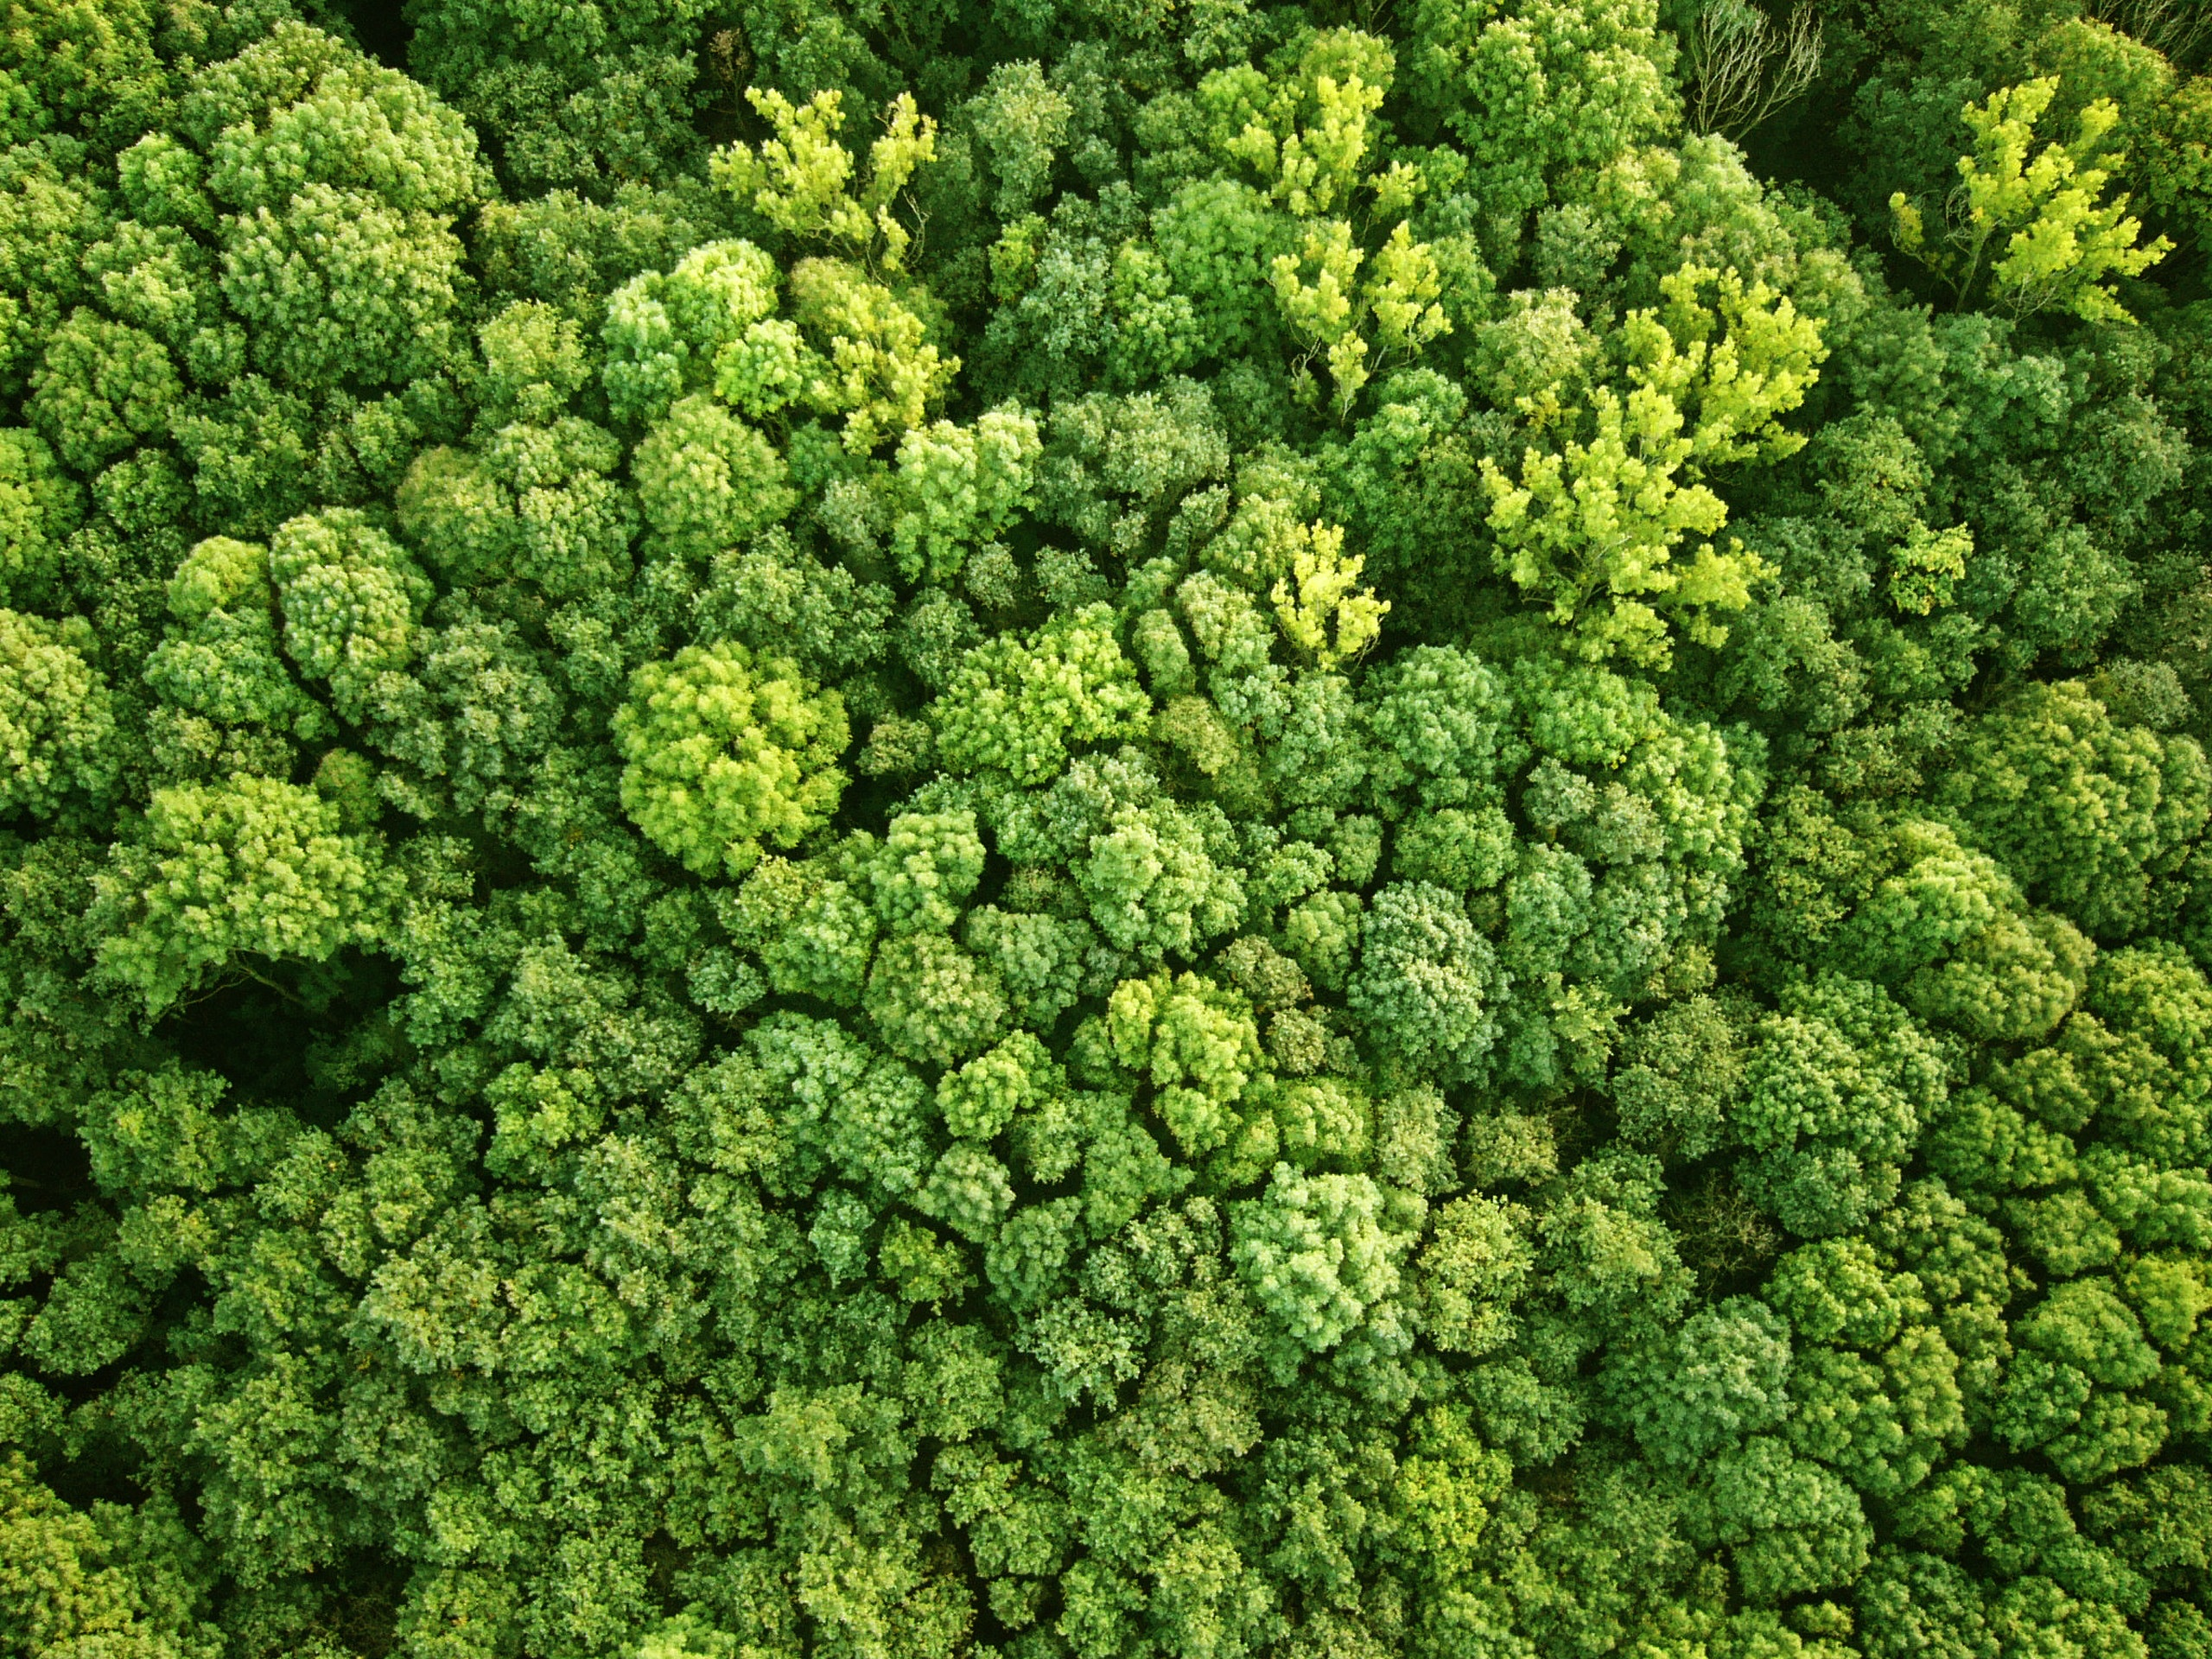
\includegraphics[keepaspectratio,
                                 width=\paperwidth]{images/forest_aerial.jpg}
            };
            \node[at=(current page.center)] {
                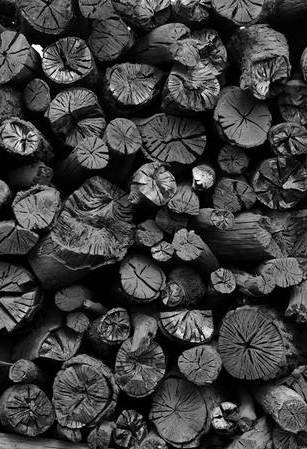
\includegraphics[keepaspectratio,
                                 height=\paperheight]{images/carbon.jpg}
            };
        \end{tikzpicture}
     \end{frame}
}


{ % all template changes are local to this group.
%%    \setbeamertemplate{navigation symbols}{}
    \begin{frame}<article:0>[plain]
      \frametitle{}
        \begin{tikzpicture}[remember picture,overlay]
            \node[at=(current page.center)] {
                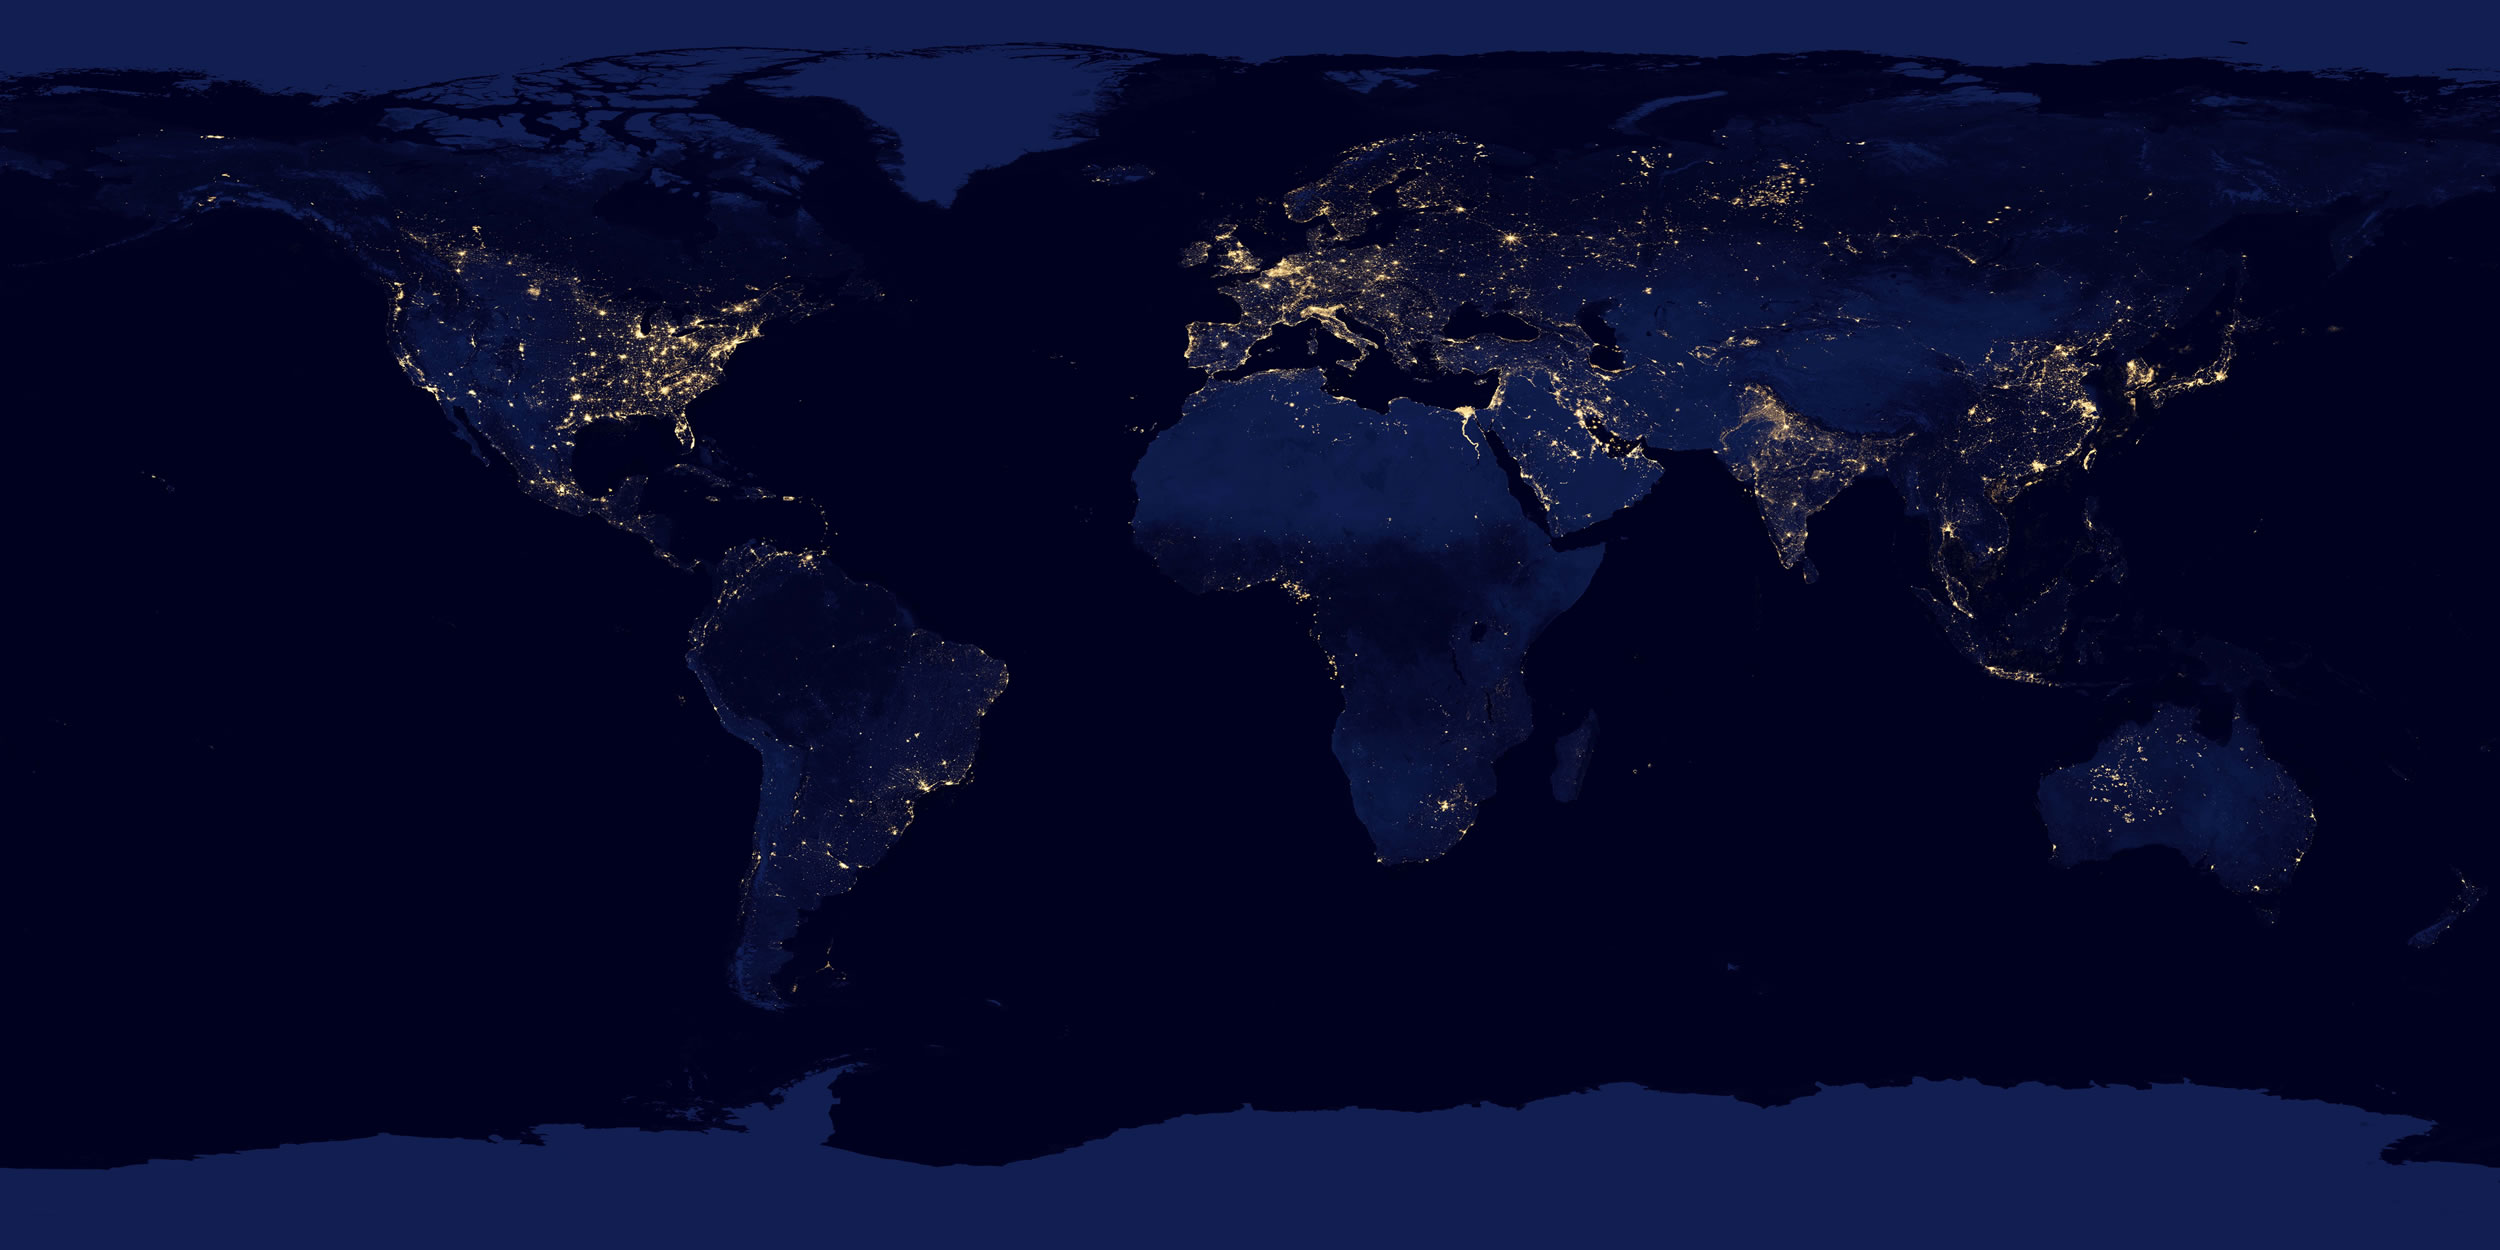
\includegraphics[keepaspectratio,
                                 height=\paperheight]{images/satellite-view-of-earth-at-night.jpg}
            };
        \end{tikzpicture}
  \note[item]{Anthropocene = proposed geological epoch distinguished by human impacts}
     \end{frame}
}



{ % all template changes are local to this group.
%%    \setbeamertemplate{navigation symbols}{}
    \begin{frame}<article:0>[plain]
      \frametitle{}
%      \cite{Ellis2020AnthropogenicCE}
        \begin{tikzpicture}[remember picture,overlay]
            \node[at=(current page.center)] {
                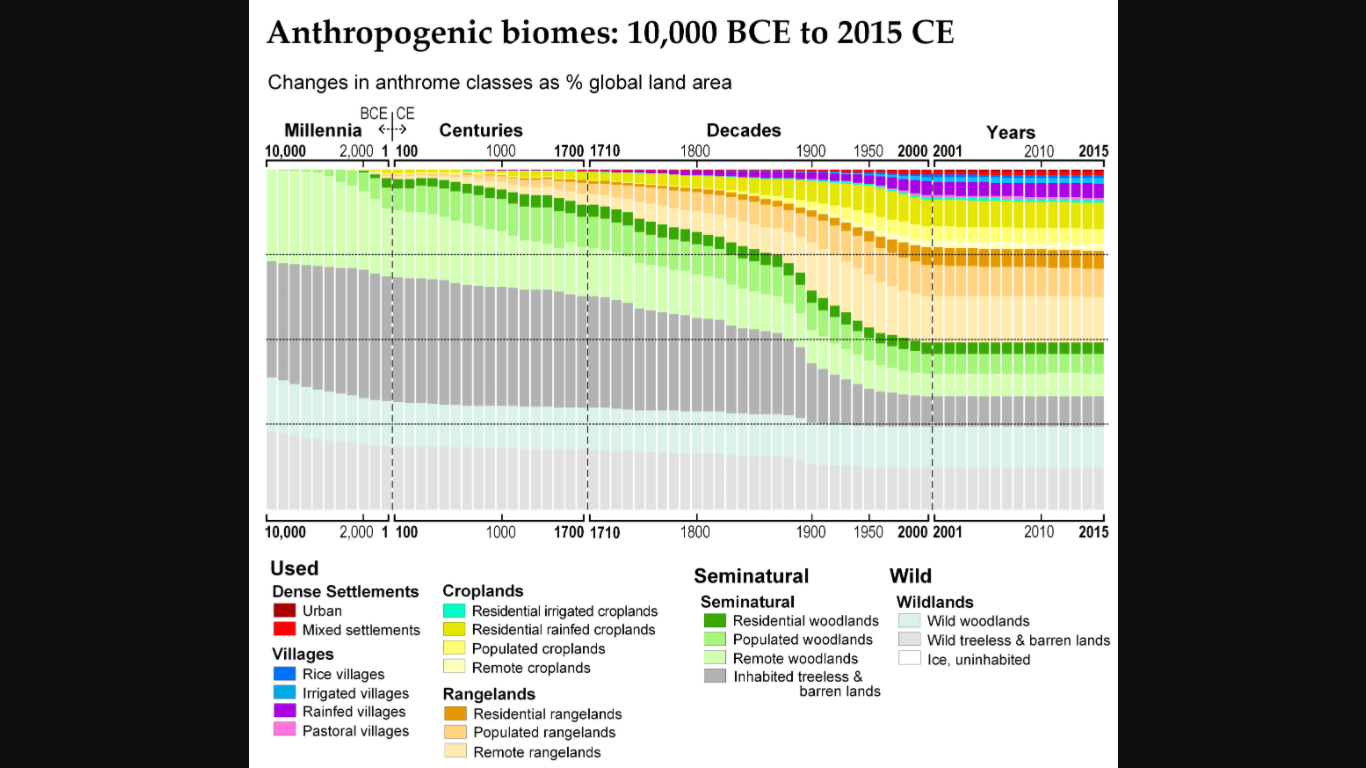
\includegraphics[keepaspectratio,
                                 width=\paperwidth,
                                 scale=0.25]{images/anthromes.png}
            };
        \end{tikzpicture}
  \note[item]{Land-use changes = conversion}
  \note[item]{One proposal is it started about 1950 with acceleration}
  \note[item]{Biodiversity changes = species introductions and extinctions}
     \end{frame}
}

{ % all template changes are local to this group.
%%    \setbeamertemplate{navigation symbols}{}
    \begin{frame}<article:0>[plain]
      \frametitle{}
        \begin{tikzpicture}[remember picture,overlay]
            \node[at=(current page.center)] {
                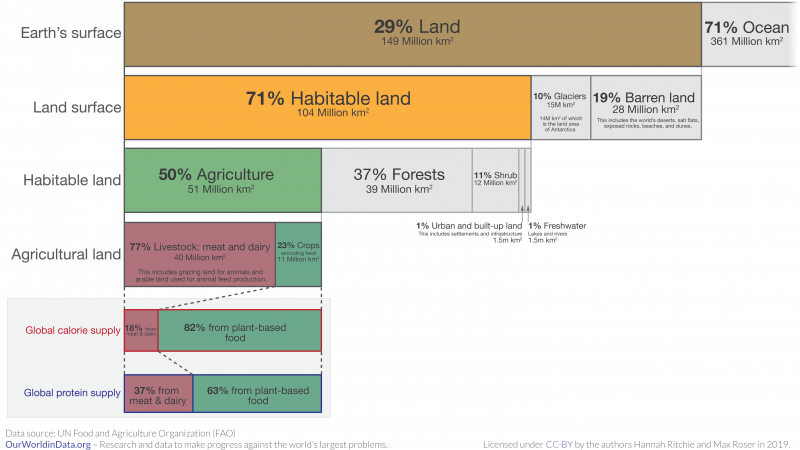
\includegraphics[keepaspectratio,
                                 width=\paperwidth,
                                 scale=0.25]{images/Global-land-use-graphic-800x506.png}
            };
        \end{tikzpicture}
  \note[item]{90\% biomass on Earth is humans and livestock}
     \end{frame}
}


{ % all template changes are local to this group.
%%    \setbeamertemplate{navigation symbols}{}
    \begin{frame}<article:0>[plain]
      \frametitle{}
        \begin{tikzpicture}[remember picture,overlay]
            \node[at=(current page.center)] {
                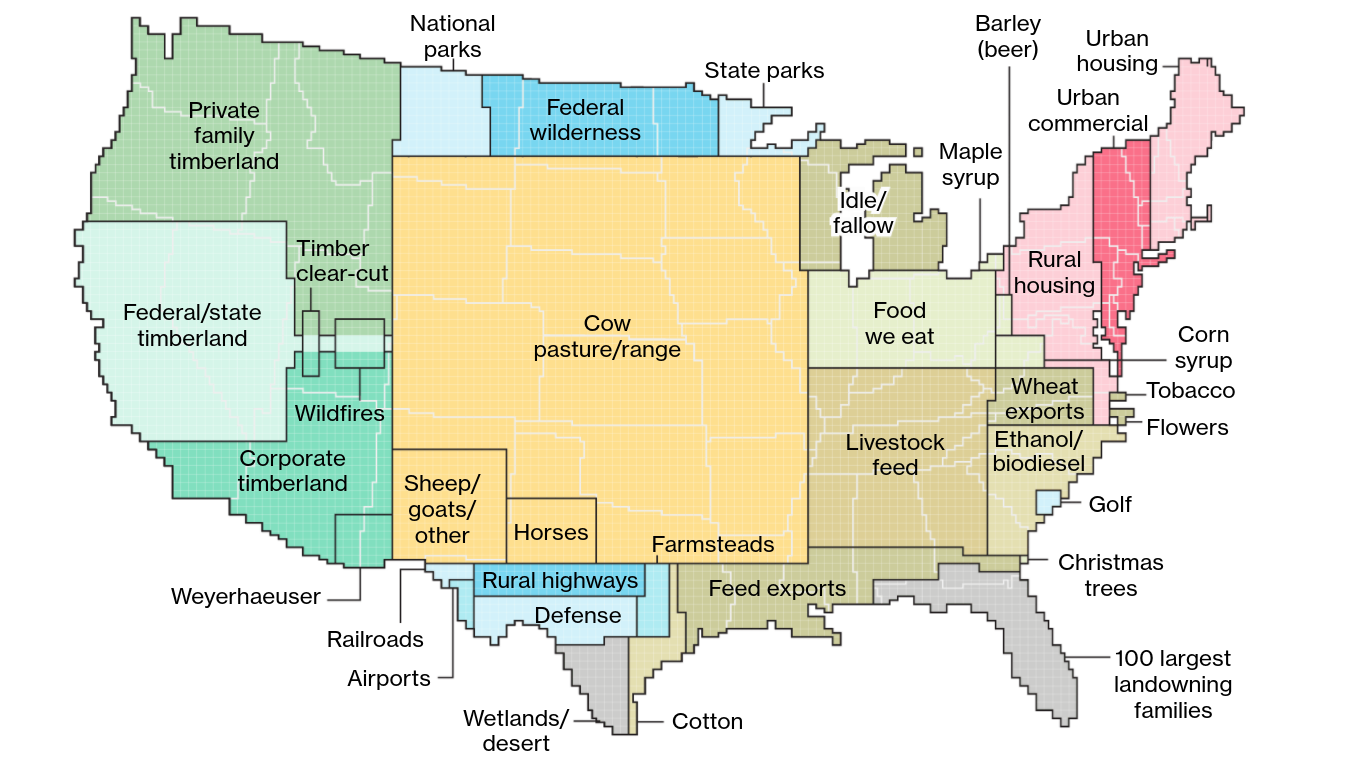
\includegraphics[keepaspectratio,
                                 width=\paperwidth]{images/how-america-uses-its-land.png}
            };
        \end{tikzpicture}
  \note[item]{90\% biomass on Earth is humans and livestock}
     \end{frame}
}




{ % all template changes are local to this group.
%%    \setbeamertemplate{navigation symbols}{}
    \begin{frame}<article:0>[plain]
      \frametitle{}
        \begin{tikzpicture}[remember picture,overlay]
            \node[at=(current page.center)] {
                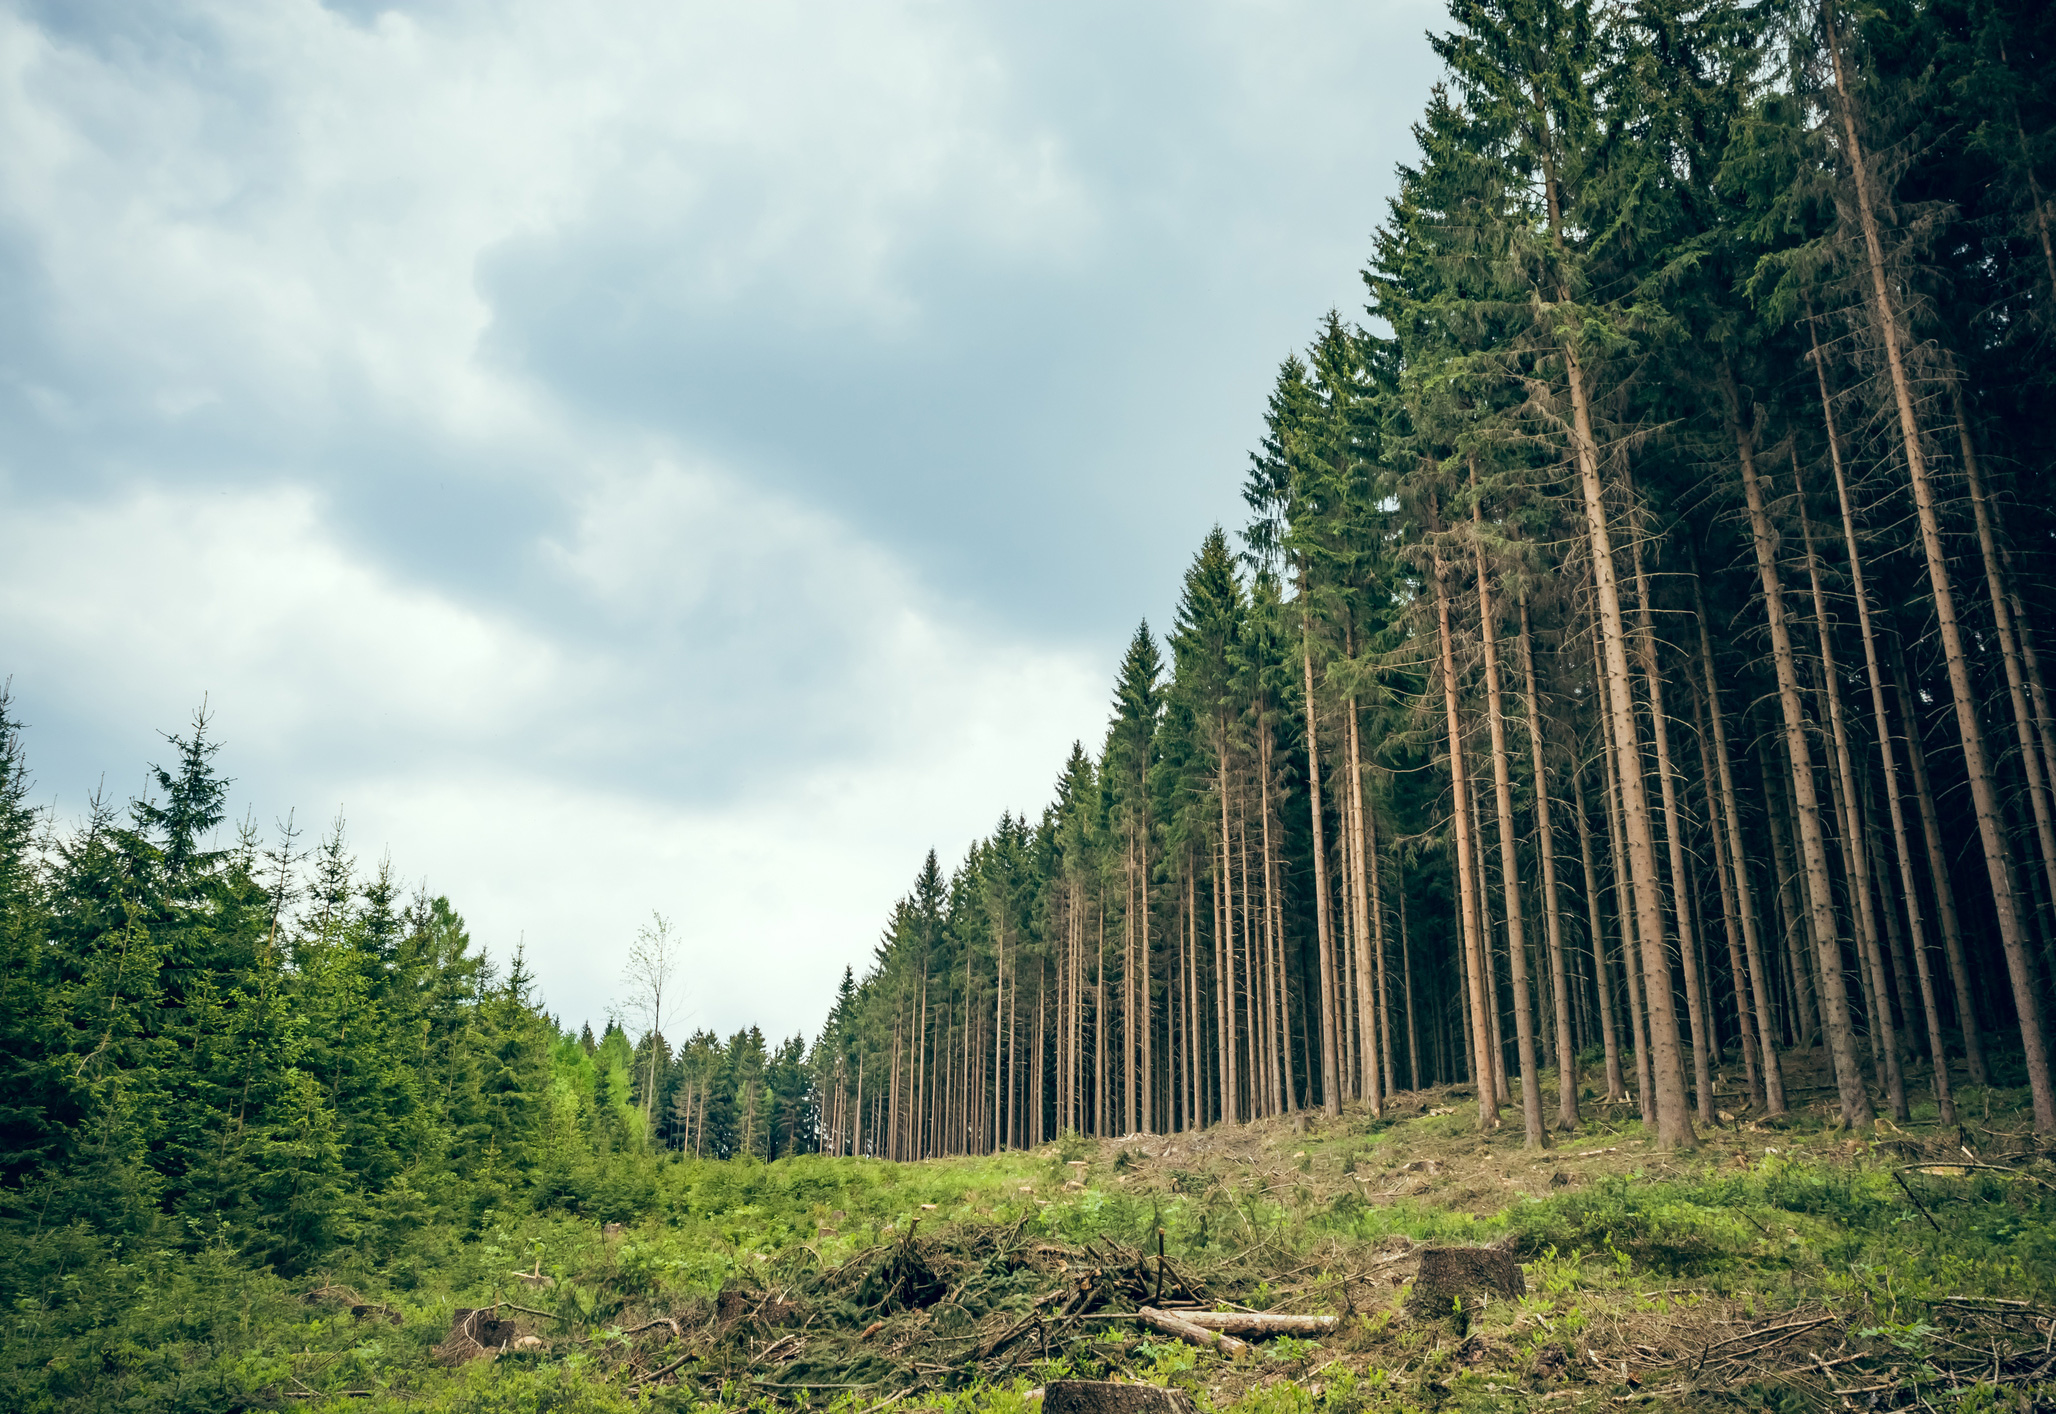
\includegraphics[keepaspectratio,
                                 width=\paperwidth]{images/forest-cut.jpg}
            };
        \end{tikzpicture}
     \end{frame}
}

{ % all template changes are local to this group.
%%    \setbeamertemplate{navigation symbols}{}
    \begin{frame}<article:0>[plain]
      \frametitle{}
        \begin{tikzpicture}[remember picture,overlay]
            \node[at=(current page.center)] {
                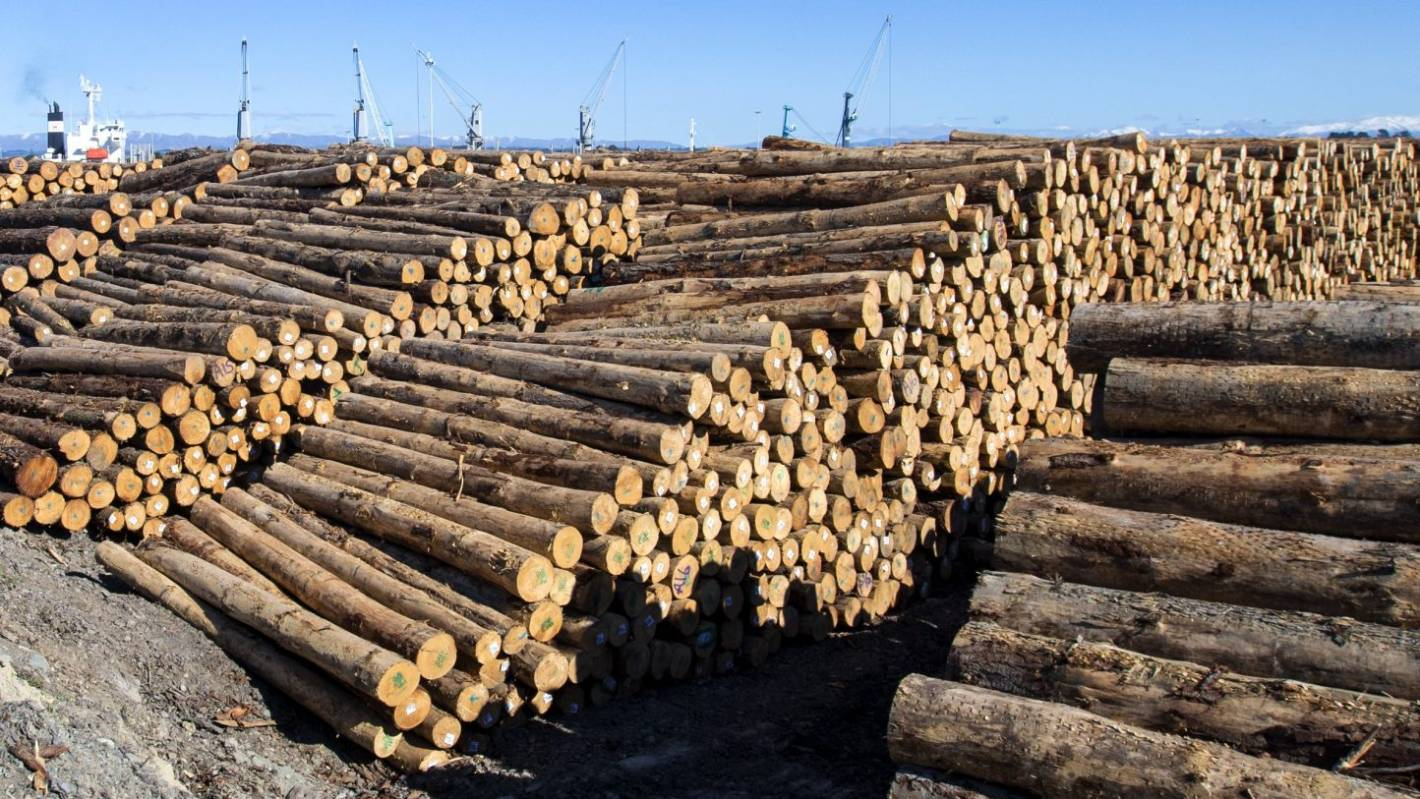
\includegraphics[keepaspectratio,
                                 width=\paperwidth]{images/sawn-logs.jpg}
            };
        \end{tikzpicture}
     \end{frame}
}






{ % all template changes are local to this group.
%%    \setbeamertemplate{navigation symbols}{}
    \begin{frame}<article:0>[plain]
      \frametitle{}
        \begin{tikzpicture}[remember picture,overlay]
            \node[at=(current page.center)] {
                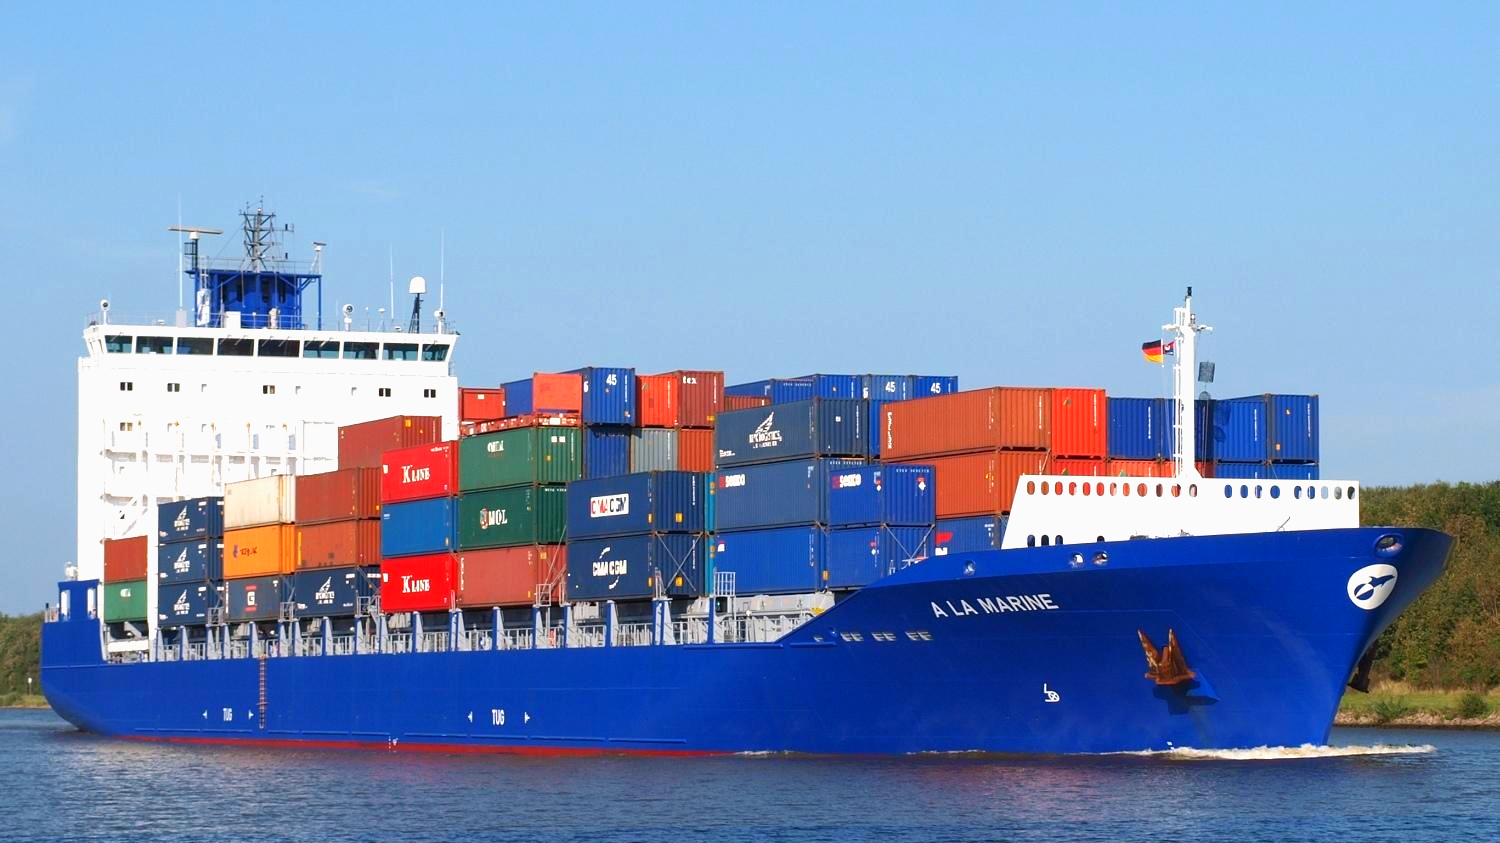
\includegraphics[keepaspectratio,
                                 width=\paperwidth]{images/shipping-ship.jpg}
            };
        \end{tikzpicture}
     \end{frame}
}


{ % all template changes are local to this group.
%%    \setbeamertemplate{navigation symbols}{}
    \begin{frame}<article:0>[plain]
      \frametitle{}
        \begin{tikzpicture}[remember picture,overlay]
            \node[at=(current page.center)] {
                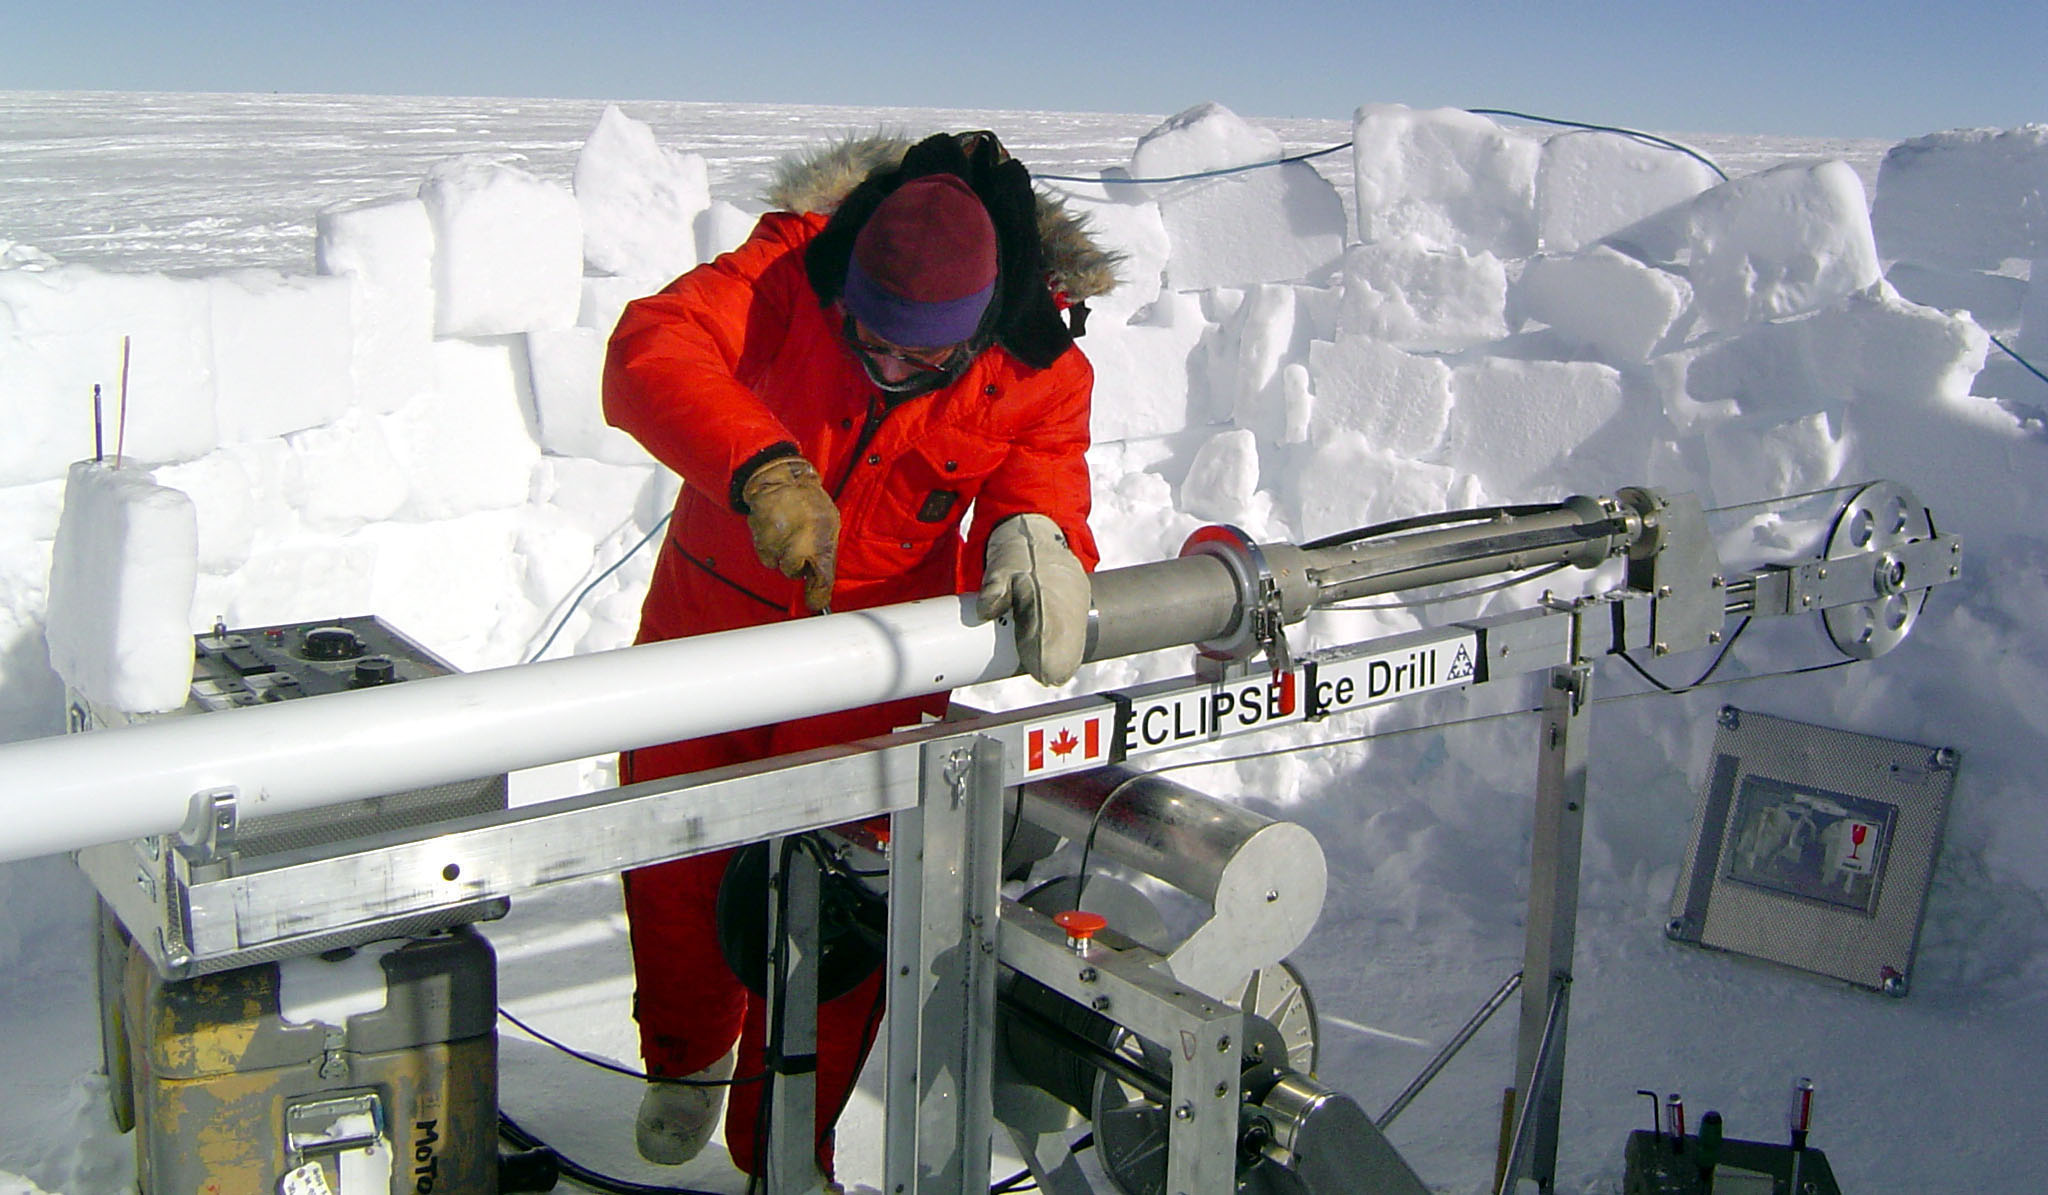
\includegraphics[keepaspectratio,
                                 width=\paperwidth]{images/ice_core.jpg}
            };
        \end{tikzpicture}
  \note[item]{Atmospheric changes = climate change, fire}
     \end{frame}
}

{ % all template changes are local to this group.
%%    \setbeamertemplate{navigation symbols}{}
    \begin{frame}<article:0>[plain]
      \frametitle{}
        \begin{tikzpicture}[remember picture,overlay]
            \node[at=(current page.center)] {
                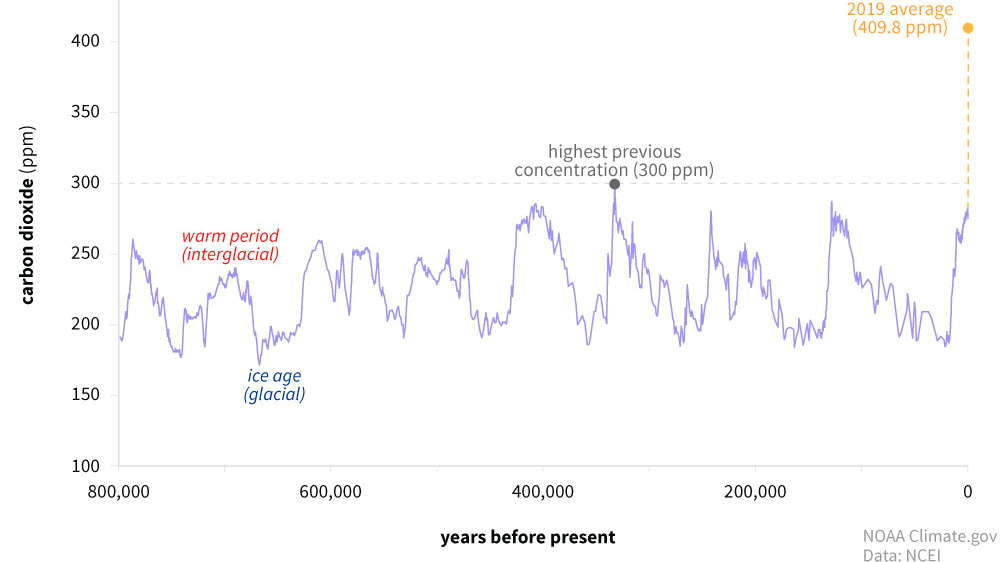
\includegraphics[keepaspectratio,
                                 width=\paperwidth]{images/BAMS_SOTC_2019_co2_paleo_1000px.jpg}
            };
        \end{tikzpicture}
     \end{frame}
}

{ % all template changes are local to this group.
%%    \setbeamertemplate{navigation symbols}{}
    \begin{frame}<article:0>[plain]
      \frametitle{}
        \begin{tikzpicture}[remember picture,overlay]
            \node[at=(current page.center)] {
                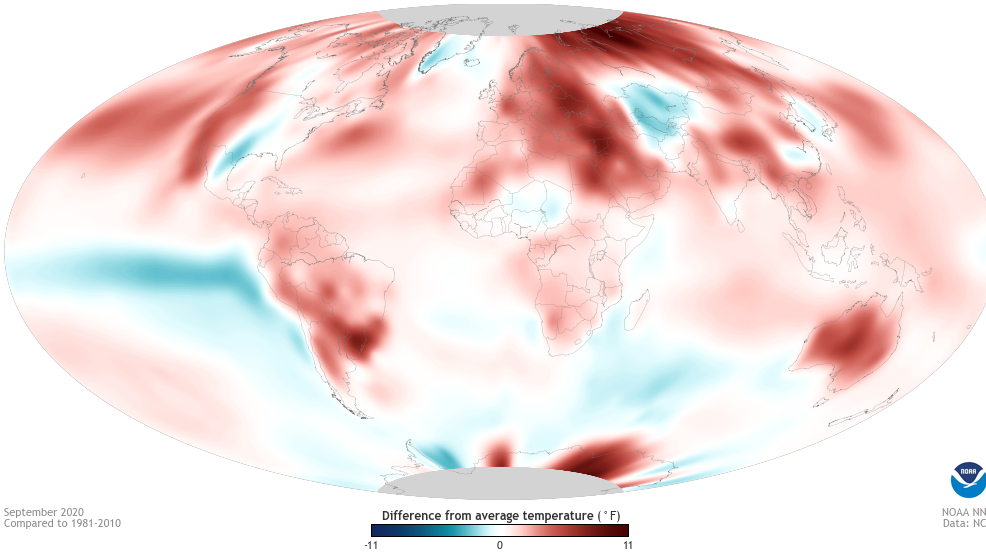
\includegraphics[keepaspectratio,
                                 width=\paperwidth]{images/September_CC2020.png}
            };
        \end{tikzpicture}
     \end{frame}
}

{ % all template changes are local to this group.
%%    \setbeamertemplate{navigation symbols}{}
    \begin{frame}<article:0>[plain]
      \frametitle{}
        \begin{tikzpicture}[remember picture,overlay]
            \node[at=(current page.center)] {
                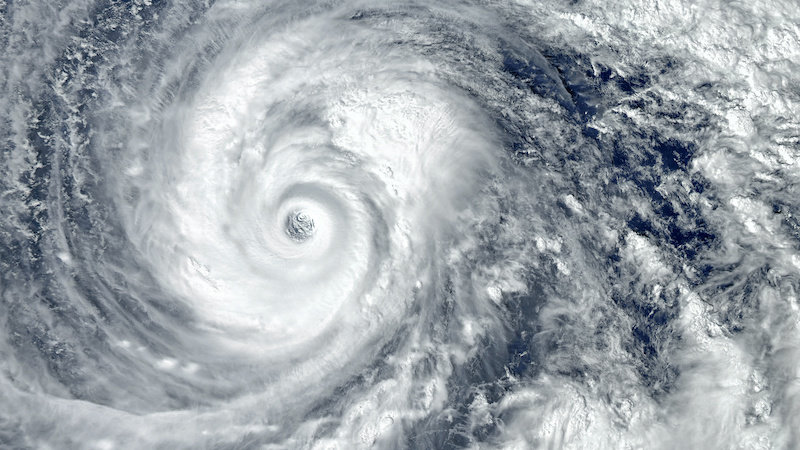
\includegraphics[keepaspectratio,
                                 width=\paperwidth]{images/hurricane.jpg}
            };
        \end{tikzpicture}
     \note[item]{Climate change is causing hurricanes that make
     landfall to take more time to weaken, reports a study published
     11th November 2020 in the journal Nature.}
     \end{frame}
}

{ % all template changes are local to this group.
%%    \setbeamertemplate{navigation symbols}{}
    \begin{frame}<article:0>[plain]
      \frametitle{}
        \begin{tikzpicture}[remember picture,overlay]
            \node[at=(current page.center)] {
                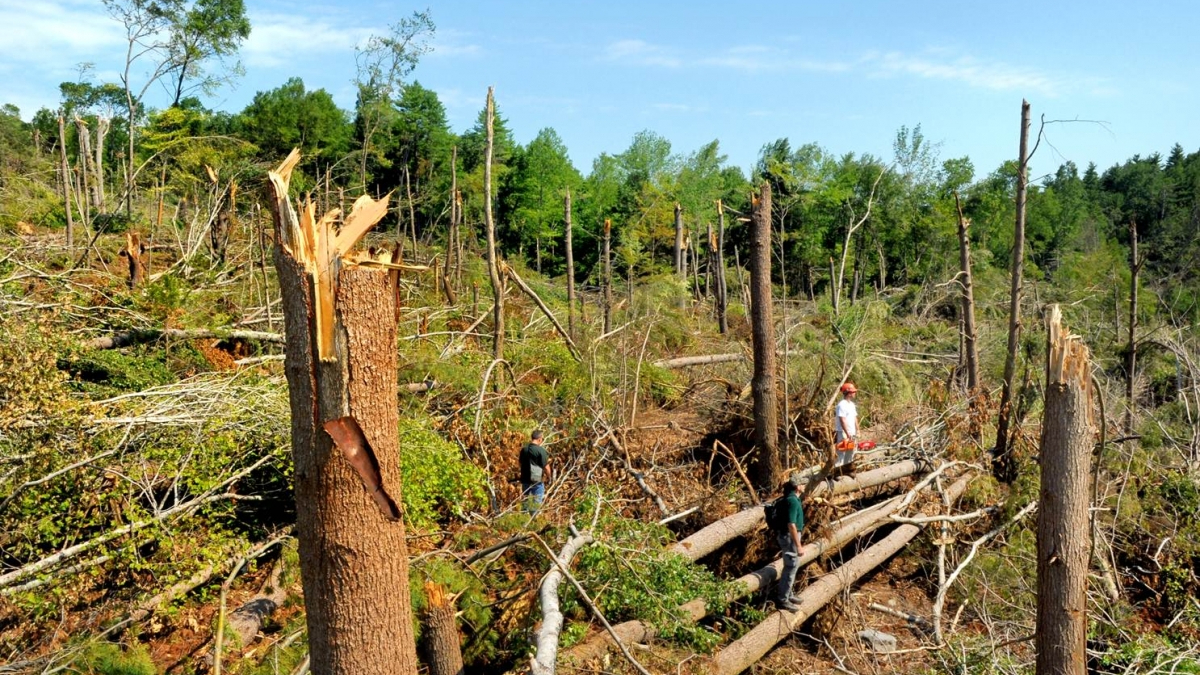
\includegraphics[keepaspectratio,
                                 width=\paperwidth]{images/tornado_hf.jpg}
            };
        \end{tikzpicture}
     \note[item]{Tornado damaged Southbridge, MA forest in 2011}
     \end{frame}
}



{ % all template changes are local to this group.
%%    \setbeamertemplate{navigation symbols}{}
    \begin{frame}<article:0>[plain]
      \frametitle{}
        \begin{tikzpicture}[remember picture,overlay]
            \node[at=(current page.center)] {
                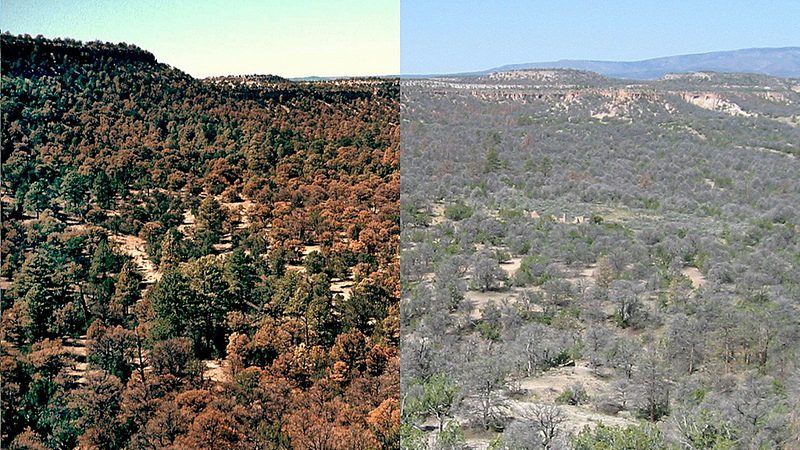
\includegraphics[keepaspectratio,
                                 width=\paperwidth]{images/drought_pjw.jpg}
            };
        \end{tikzpicture}
        \note[item]{Droughts}
     \end{frame}
}



{ % all template changes are local to this group.
%%    \setbeamertemplate{navigation symbols}{}
    \begin{frame}<article:0>[plain]
      \frametitle{}
        \begin{tikzpicture}[remember picture,overlay]
            \node[at=(current page.center)] {
                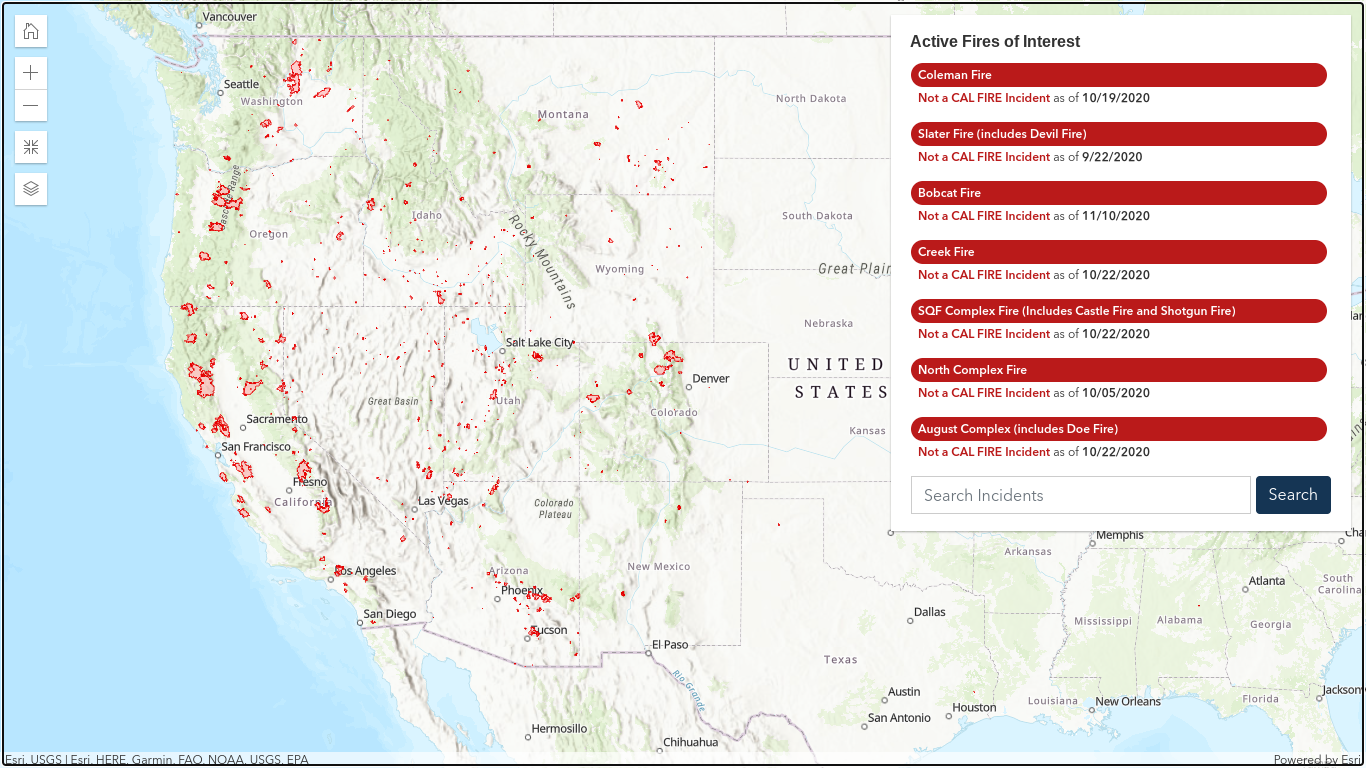
\includegraphics[keepaspectratio,
                                  width=\paperwidth]{images/fires_CALFIRE.png}
            };
        \end{tikzpicture}
        \note[item]{CAL FIRE MAP Tue 17 Nov 2020 12:10:52 PM EST}
     \end{frame}
}


{ % all template changes are local to this group.
%%    \setbeamertemplate{navigation symbols}{}
    \begin{frame}<article:0>[plain]
      \frametitle{}
        \begin{tikzpicture}[remember picture,overlay]
            \node[at=(current page.center)] {
                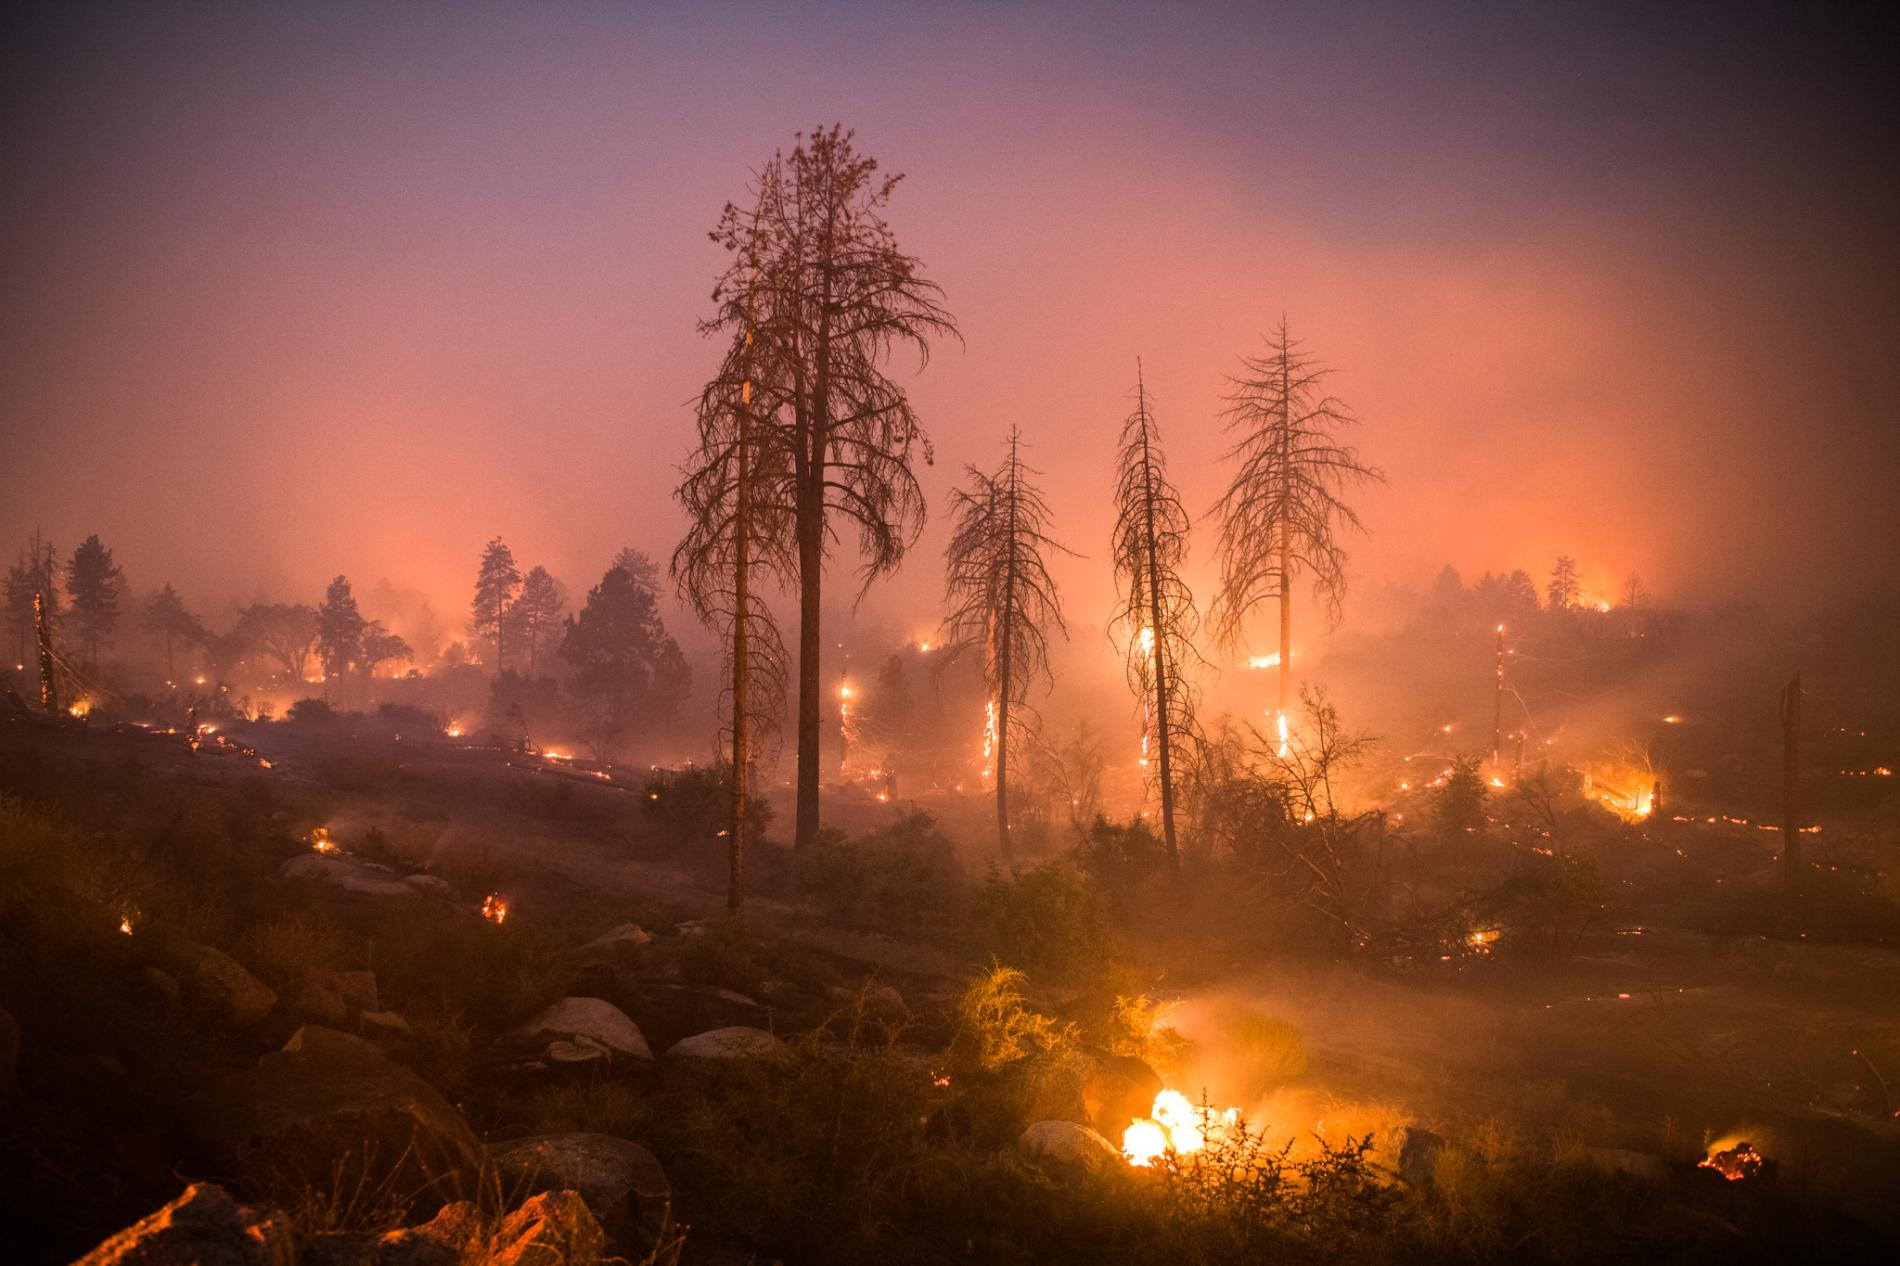
\includegraphics[keepaspectratio,
                                 width=\paperwidth]{images/fires_CAcranston.jpg}
            };
        \end{tikzpicture}
        \note[item]{CA Cranston Riverside 2018}
     \end{frame}
}


{ % all template changes are local to this group.
%%    \setbeamertemplate{navigation symbols}{}
    \begin{frame}<article:0>[plain]
      \frametitle{}
        \begin{tikzpicture}[remember picture,overlay]
            \node[at=(current page.center)] {
                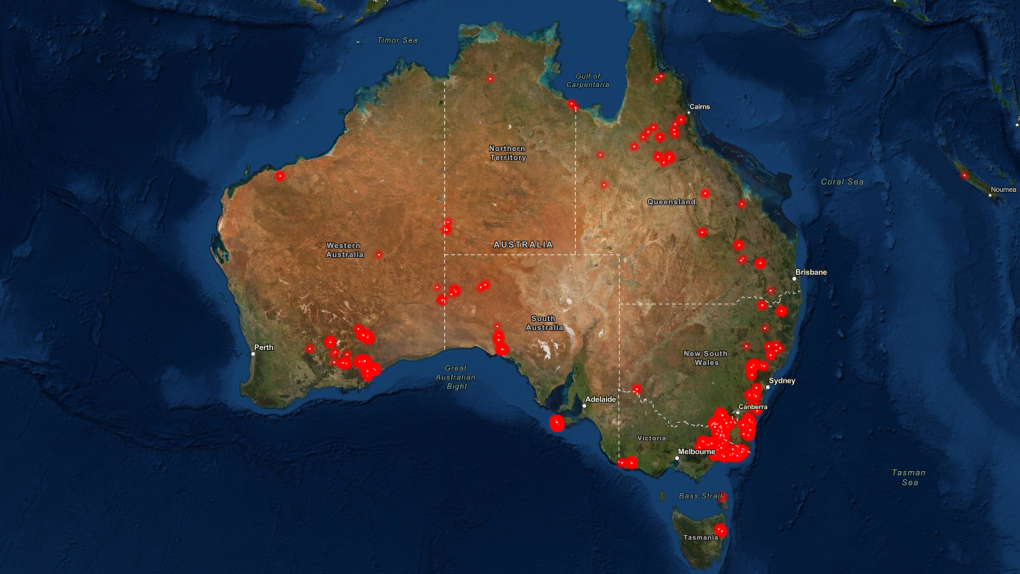
\includegraphics[keepaspectratio,
                                 width=\paperwidth]{images/fires_AUS.png}
            };
        \end{tikzpicture}
        \note[item]{Fires in Australia 2020}
     \end{frame}
}







\begin{frame}
  \frametitle{Forests in the Anthropocence}
  
  \begin{itemize}
  \item Forests are changing from human impacts \pause
  \item Large direct and \underline{indirect} effects of land-use  \pause
  \item How do we address indirect and systems-level effects? 
  \end{itemize}

\end{frame}


\begin{frame}
  \frametitle{Today's Talk}

\tableofcontents

\note[item]{Intro/Context}
\note[item]{Global forest loss and gain and change}
\note[item]{Global greening = India(Agriculture) + China(Forests)}
\note[item]{Economics*Ecology = Landscape Extended Models}
\note[item]{Network Analysis of China's Greening}
\note[item]{Global Scale}
\note[item]{Local Scale}
\note[item]{Landscape = Tian 2019, Chen 2019}
\note[item]{Resilience Analysis of China's Forest LE-MRIO}
\note[item]{Conclusions and Future Work}
\note[item]{Acknowledgements}

\end{frame}



\section{Environmentally Extended Economic Models}


\begin{frame}
  \frametitle{Economic Input-Output Models}
\end{frame}



{ 
\begin{frame}<article:0>[plain]
   \frametitle{}
      \begin{tikzpicture}[remember picture,overlay]
         \node[at=(current page.center)] {
             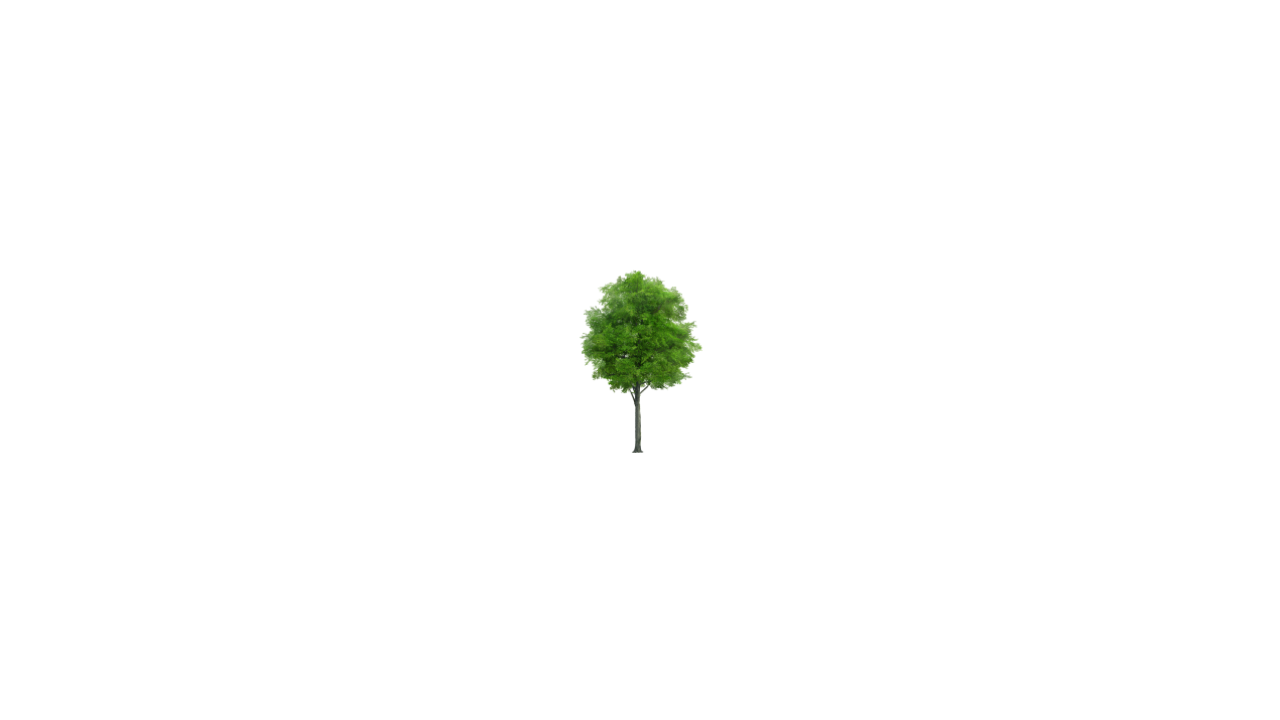
\includegraphics[keepaspectratio,
                              width=\paperwidth]{images/le-mrio.png}
            };
      \end{tikzpicture}
     \note[]{When we think about environmental impacts of humans, we
      usually think about direct impacts}
\end{frame}
}




{ 
\begin{frame}<article:0>[plain]
   \frametitle{}
      \begin{tikzpicture}[remember picture,overlay]
         \node[at=(current page.center)] {
             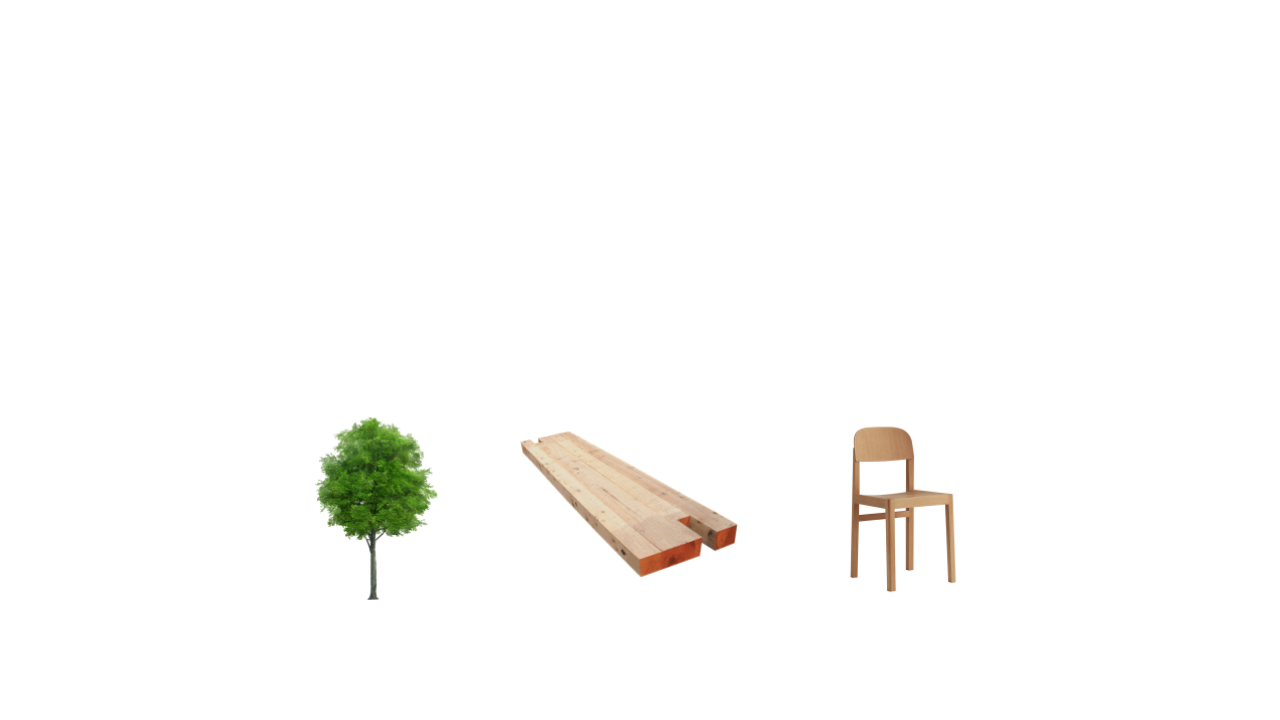
\includegraphics[keepaspectratio,
                              width=\paperwidth]{images/le-mrio-3.png}
            };
      \end{tikzpicture}
     \note[]{}
\end{frame}
}



{ 
\begin{frame}<article:0>[plain]
   \frametitle{}
      \begin{tikzpicture}[remember picture,overlay]
         \node[at=(current page.center)] {
             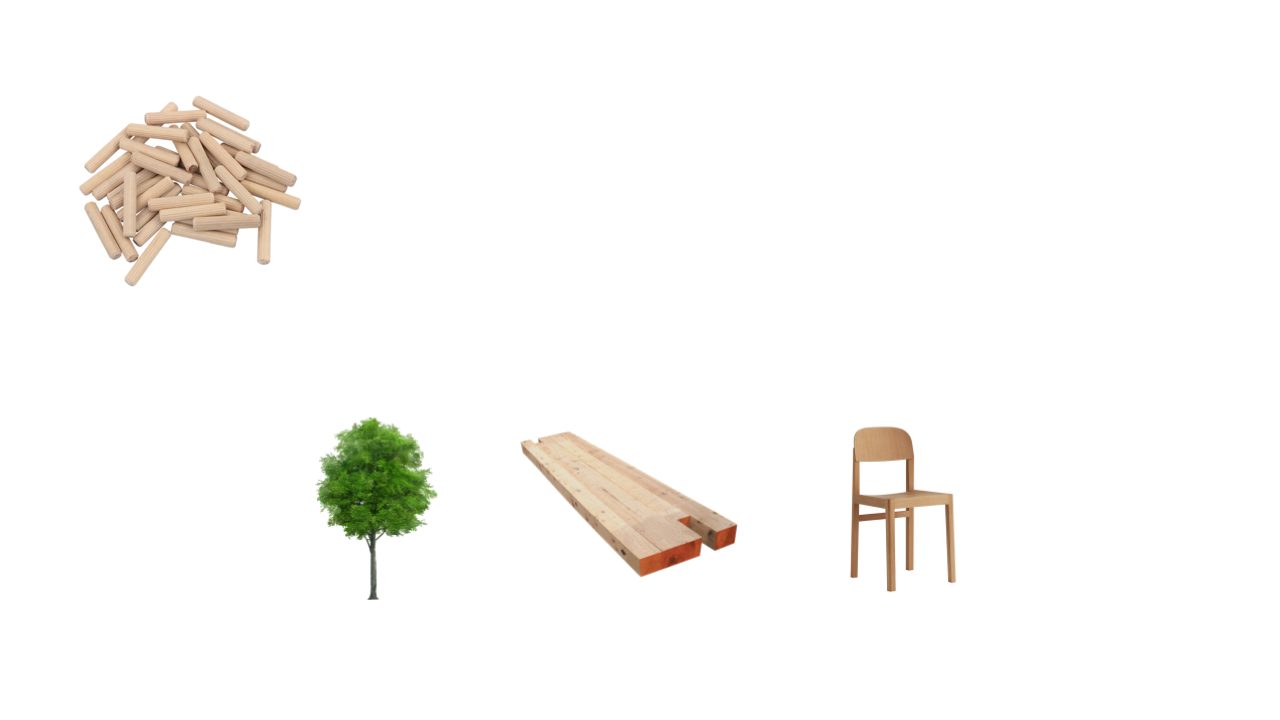
\includegraphics[keepaspectratio,
                              width=\paperwidth]{images/le-mrio-4.png}
            };
      \end{tikzpicture}
     \note[]{}
\end{frame}
}



{ 
\begin{frame}<article:0>[plain]
   \frametitle{}
      \begin{tikzpicture}[remember picture,overlay]
         \node[at=(current page.center)] {
             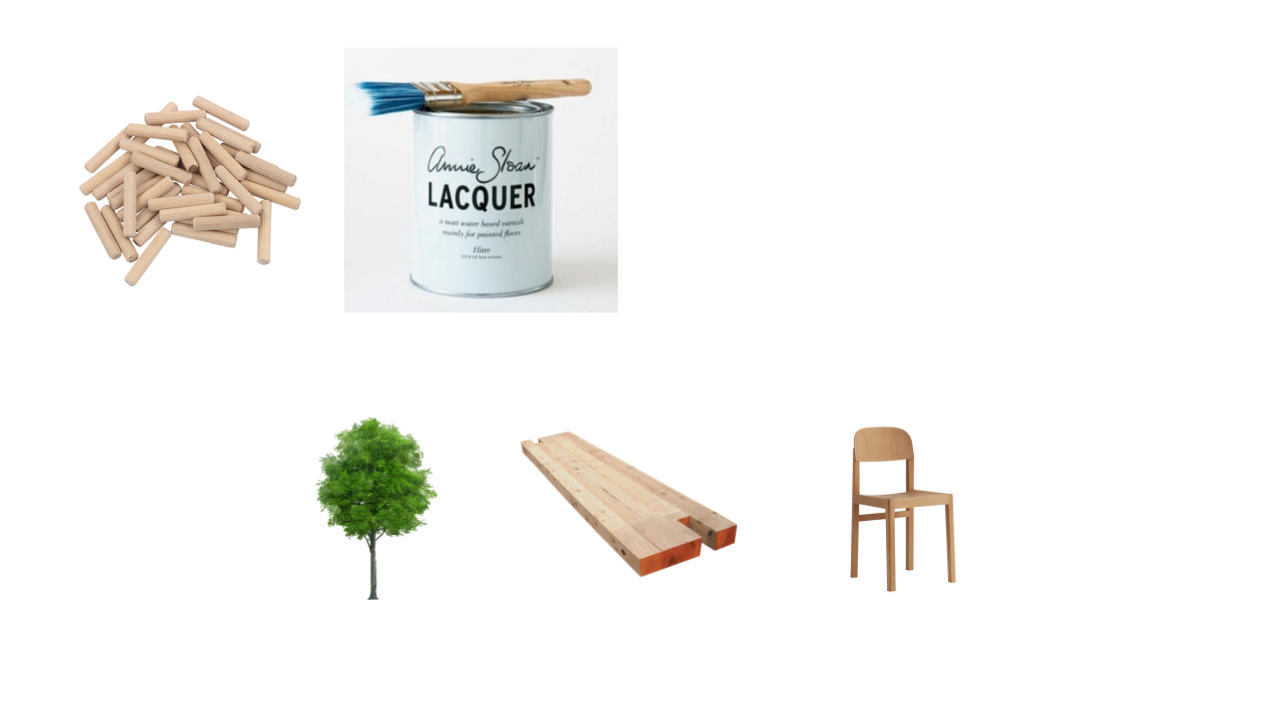
\includegraphics[keepaspectratio,
                              width=\paperwidth]{images/le-mrio-5.png}
            };
      \end{tikzpicture}
     \note[]{}
\end{frame}
}



{ 
\begin{frame}<article:0>[plain]
   \frametitle{}
      \begin{tikzpicture}[remember picture,overlay]
         \node[at=(current page.center)] {
             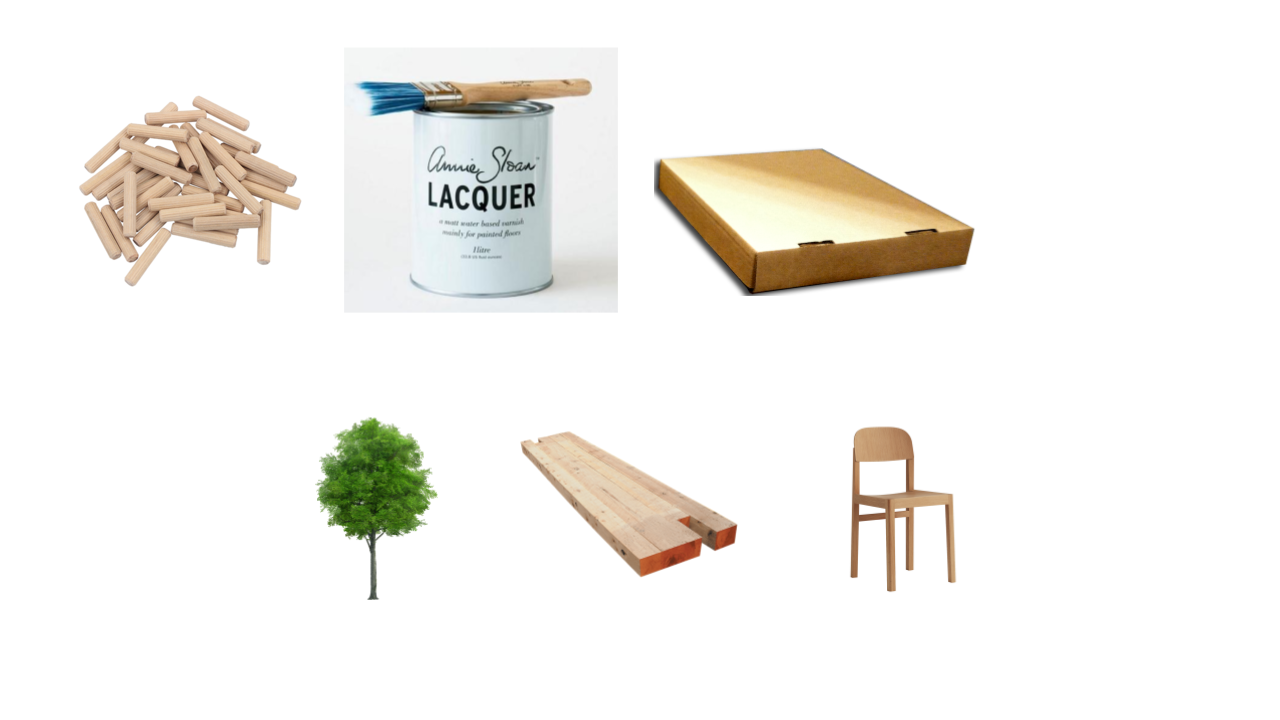
\includegraphics[keepaspectratio,
                              width=\paperwidth]{images/le-mrio-6.png}
            };
      \end{tikzpicture}
     \note[]{}
\end{frame}
}



{ 
\begin{frame}<article:0>[plain]
   \frametitle{}
      \begin{tikzpicture}[remember picture,overlay]
         \node[at=(current page.center)] {
             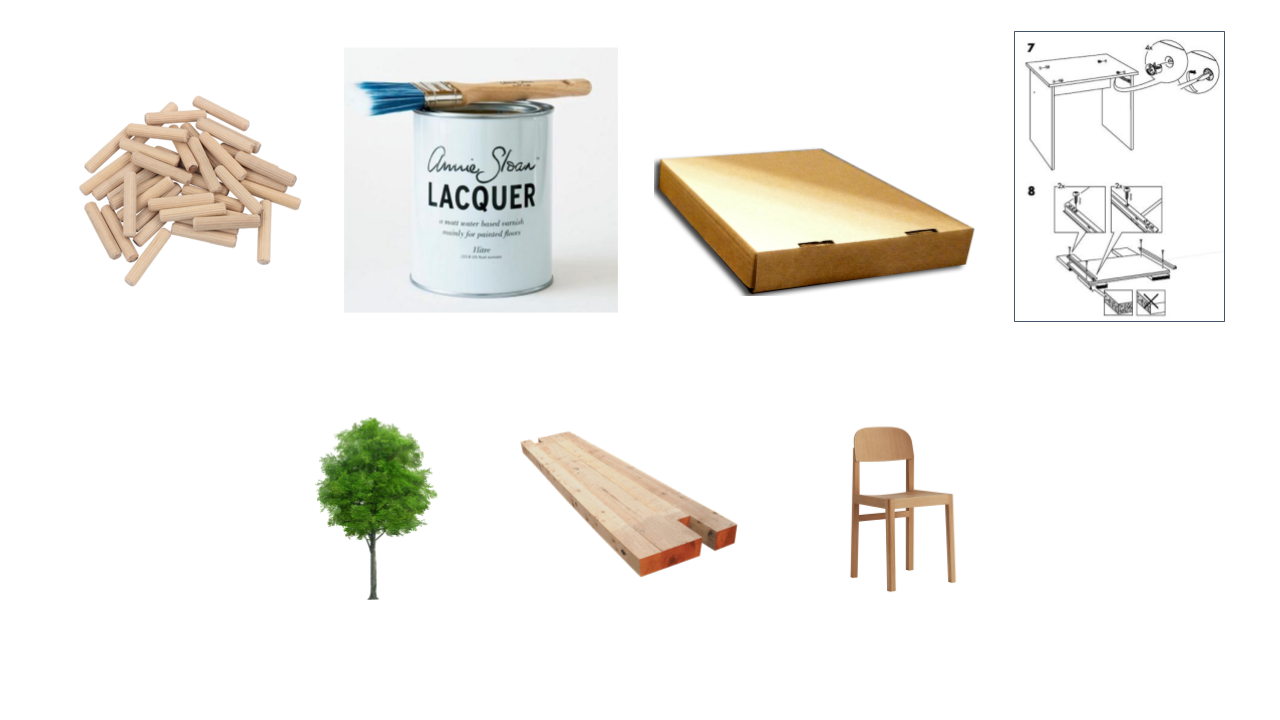
\includegraphics[keepaspectratio,
                              width=\paperwidth]{images/le-mrio-7.png}
            };
      \end{tikzpicture}
     \note[]{}
\end{frame}
}

{ 
\begin{frame}<article:0>[plain]
   \frametitle{}
      \begin{tikzpicture}[remember picture,overlay]
         \node[at=(current page.center)] {
             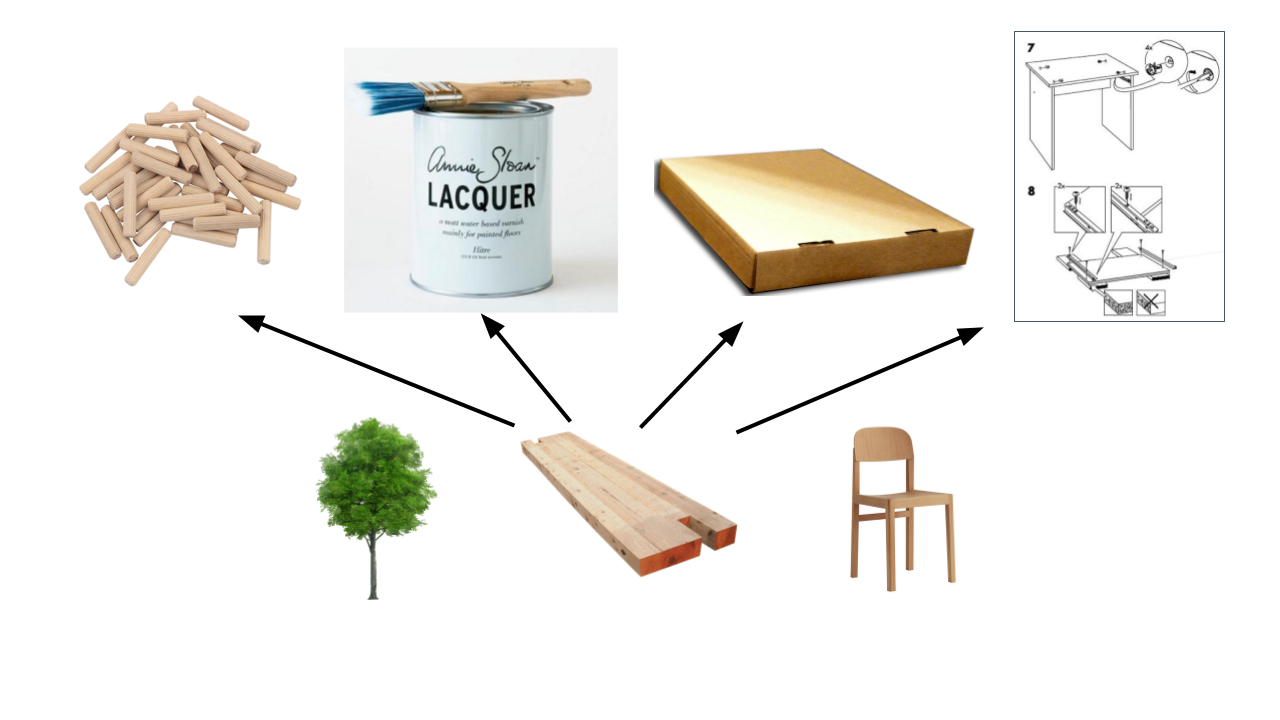
\includegraphics[keepaspectratio,
                              width=\paperwidth]{images/le-mrio-8.png}
            };
      \end{tikzpicture}
     \note[]{}
\end{frame}
}

{ 
\begin{frame}<article:0>[plain]
   \frametitle{}
      \begin{tikzpicture}[remember picture,overlay]
         \node[at=(current page.center)] {
             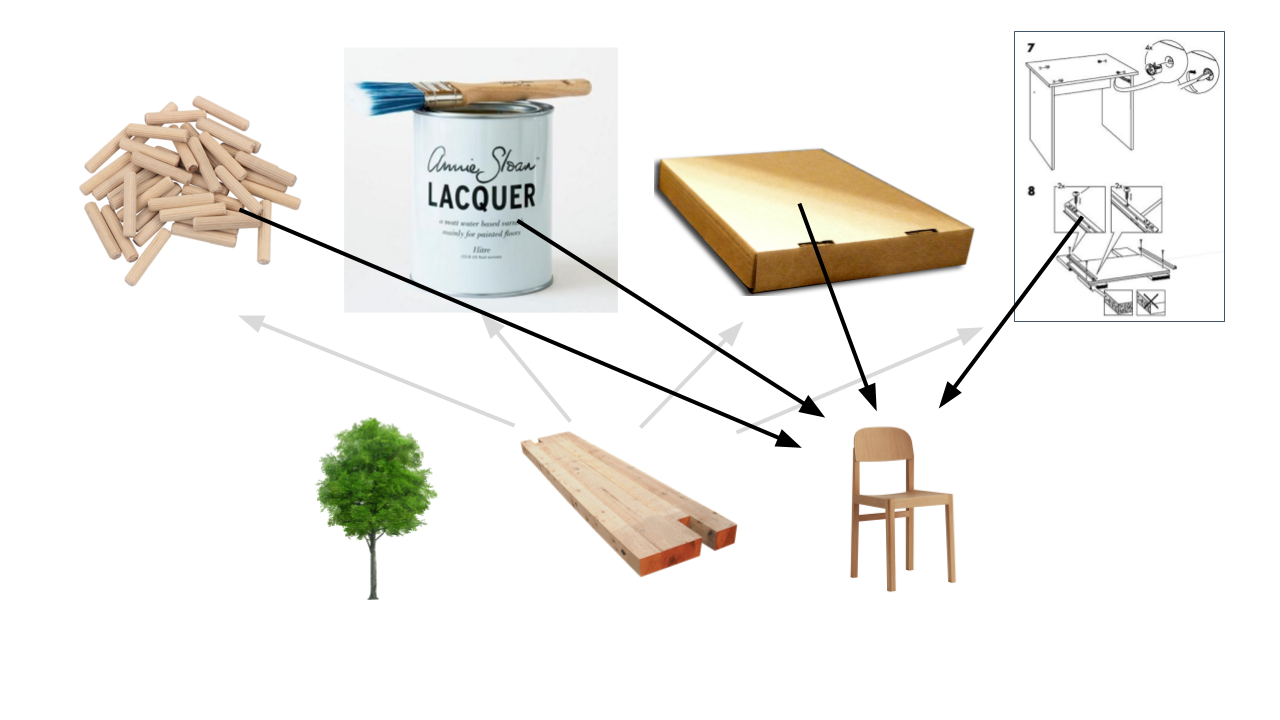
\includegraphics[keepaspectratio,
                              width=\paperwidth]{images/le-mrio-9.png}
            };
      \end{tikzpicture}
     \note[]{}
\end{frame}
}

\begin{frame}
  \frametitle{Economic Input-Output Modeling}
\begin{columns}
\begin{column}{0.5\textwidth}
\begin{center}
$X = (I - A)^{-1}Y$
\end{center}
\end{column}
\begin{column}{0.5\textwidth}  %%<--- here
\end{column}
\end{columns}
\end{frame}

\begin{frame}
  \frametitle{Economic Input-Output Modeling}
\begin{columns}
\begin{column}{0.5\textwidth}
\begin{center}
$X = (I - A)^{-1}Y$
\\ 
\begin{itemize}
\item $X$: total consumption \pause
\item $A$: intermediate consumption \pause
\item $Y$: final use \pause
\item $I$: identity matrix 
\end{itemize}
\end{center}
\end{column}
\begin{column}{0.5\textwidth}  %%<--- here
\end{column}
\end{columns}
\end{frame}


\begin{frame}
  \frametitle{Economic Input-Output Modeling}
\begin{columns}
\begin{column}{0.5\textwidth}
\begin{center}
$X = (I - A)^{-1}Y$
\\ 
\begin{itemize}
\item $X$: total consumption 
\item $A$: intermediate consumption
\item $Y$: final use 
\item $I$: identity matrix 
\end{itemize}
\end{center}
\end{column}
\begin{column}{0.5\textwidth}  %%<--- here
  \begin{itemize}
  \item Wassily Leontief (1936)
  \item \textit{Leontief Inverse} $(I - A)^{-1}$ calculates all of the indirect
  consumption correctly \pause
  \item Indirect effects can, and usually are, greater than direct \pause
  \item Has been influential in ecosystem network analysis
  \end{itemize}
\end{column}
\end{columns}
\end{frame}


\begin{frame}
  \frametitle{Environmental Extended Input-Output Models}
\begin{columns}
\begin{column}{0.5\textwidth}
\begin{center}
$X = (I - A)^{-1}Y$
\end{center}
\end{column}
\begin{column}{0.5\textwidth}  %%<--- here

\end{column}
\end{columns}
\end{frame}

\begin{frame}
  \frametitle{Environmental Extended Input-Output Models}
\begin{columns}
\begin{column}{0.5\textwidth}
\begin{center}
$E = F(I - A)^{-1}Y$
\end{center}
\end{column}
\begin{column}{0.5\textwidth}  %%<--- here

\end{column}
\end{columns}
\end{frame}


\begin{frame}
  \frametitle{Environmental Extended Input-Output Models}
\begin{columns}
\begin{column}{0.5\textwidth}
\begin{center}
$E = F(I - A)^{-1}Y$
\\
\begin{itemize}
\item $F$: environmental inputs \pause
\item $E$: environmental consumption
\end{itemize}
\end{center}
\end{column}
\begin{column}{0.5\textwidth}  %%<--- here
\end{column}
\end{columns}
\end{frame}

\begin{frame}
  \frametitle{Environmental Extended Input-Output Models}
\begin{columns}
\begin{column}{0.5\textwidth}
\begin{center}
$E = F(I - A)^{-1}Y$
\\
\begin{itemize}
\item $F$: environmental inputs 
\item $E$: environmental consumption
\end{itemize}
\end{center}
\end{column}
\begin{column}{0.5\textwidth}  %%<--- here
  \begin{itemize}
  \item Any environmental (or social) variable can be used \pause
  \item \textbf{Required}: estimate of how much is used by each
  industrial sector
  \end{itemize}
\end{column}
\end{columns}
\end{frame}

{ 
\begin{frame}<article:0>[plain]
   \frametitle{}
      \begin{tikzpicture}[remember picture,overlay]
         \node[at=(current page.center)] {
             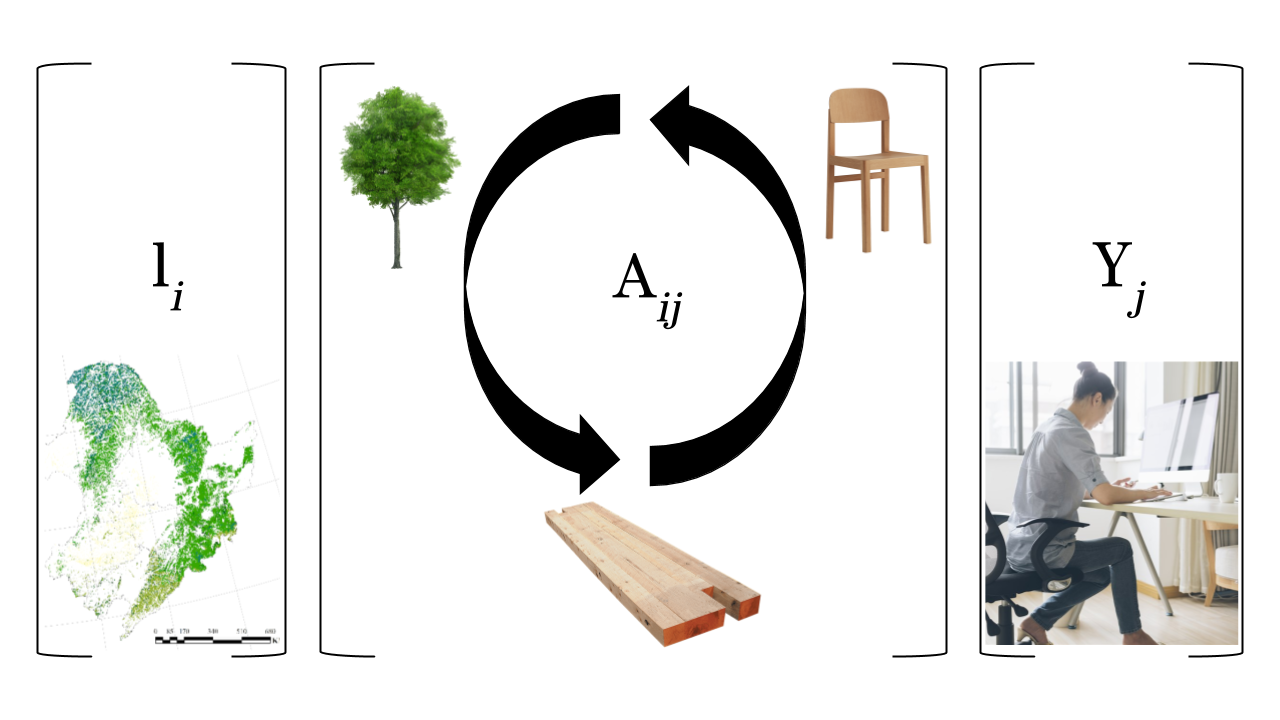
\includegraphics[keepaspectratio,
                              width=\paperwidth]{images/le-mrio-form.png}
            };
      \end{tikzpicture}
     \note[item]{For the rest of the talk, I'll usually refer to
      landscape networks, which means the proportion of landscape
      ultimately used to produce a product considering all of the
      indirect production pathways (aka. supply chains)}
\end{frame}
}



\begin{frame}
  \frametitle{``Multi-Regional'' = Spatial Context}
\end{frame}


{ %%% blank frame
\begin{frame}<article:0>[plain]
   \frametitle{}
      \begin{tikzpicture}[remember picture,overlay]
         \node[at=(current page.center)] {
             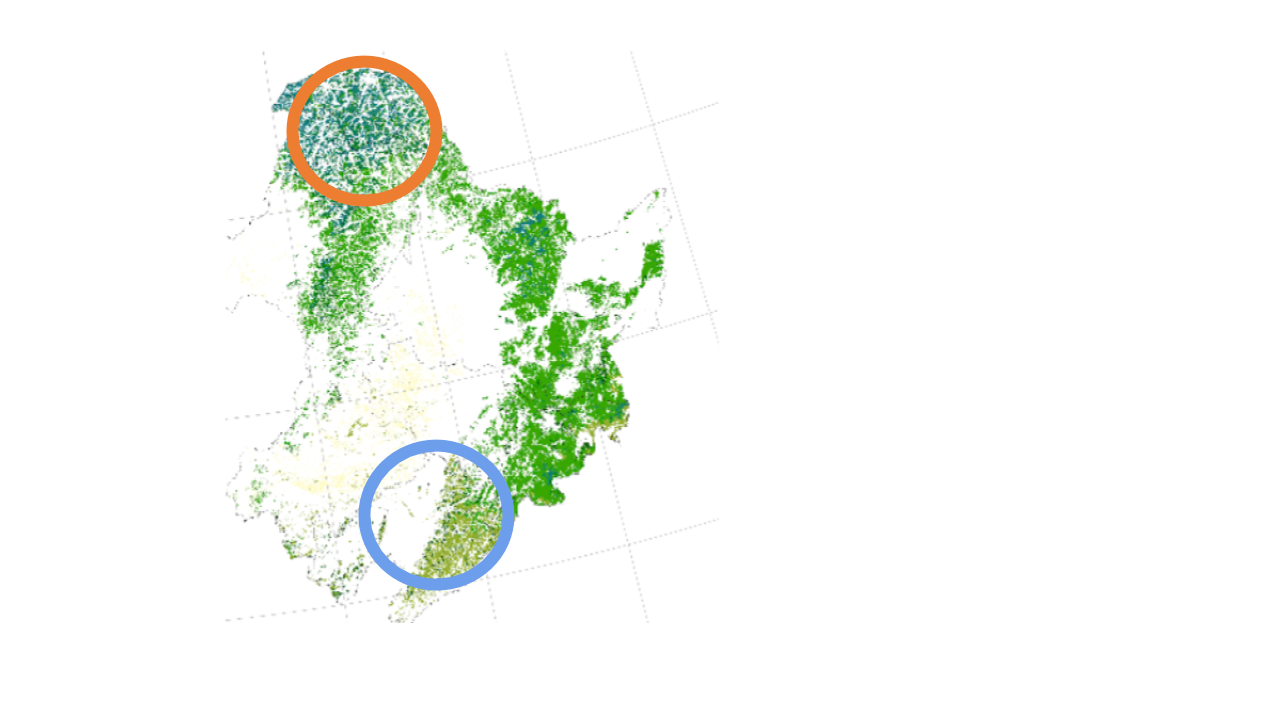
\includegraphics[keepaspectratio,
                              width=\paperwidth]{images/regionalize1.png}
            };
      \end{tikzpicture}
     \note[]{}
\end{frame}
}

{ %%% blank frame
\begin{frame}<article:0>[plain]
   \frametitle{}
      \begin{tikzpicture}[remember picture,overlay]
         \node[at=(current page.center)] {
             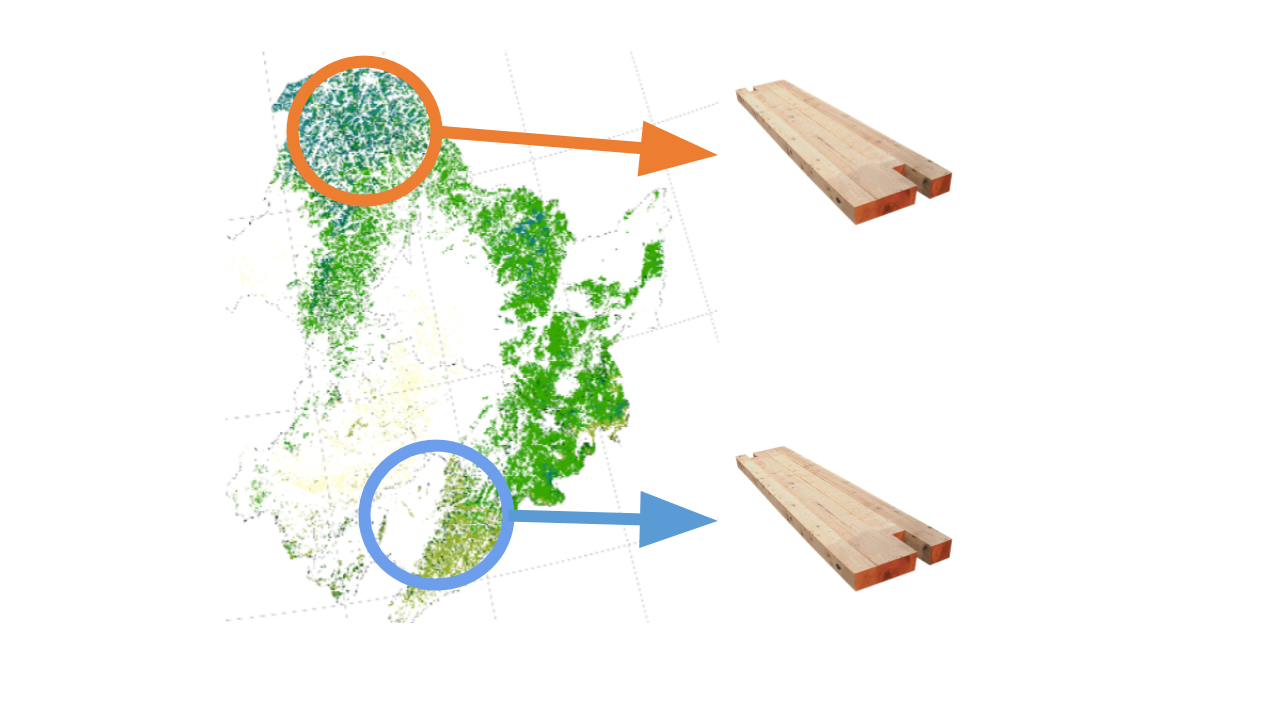
\includegraphics[keepaspectratio,
                              width=\paperwidth]{images/regionalize2.png}
            };
      \end{tikzpicture}
     \note[]{}
\end{frame}
}

{ %%% blank frame
\begin{frame}<article:0>[plain]
   \frametitle{}
      \begin{tikzpicture}[remember picture,overlay]
         \node[at=(current page.center)] {
             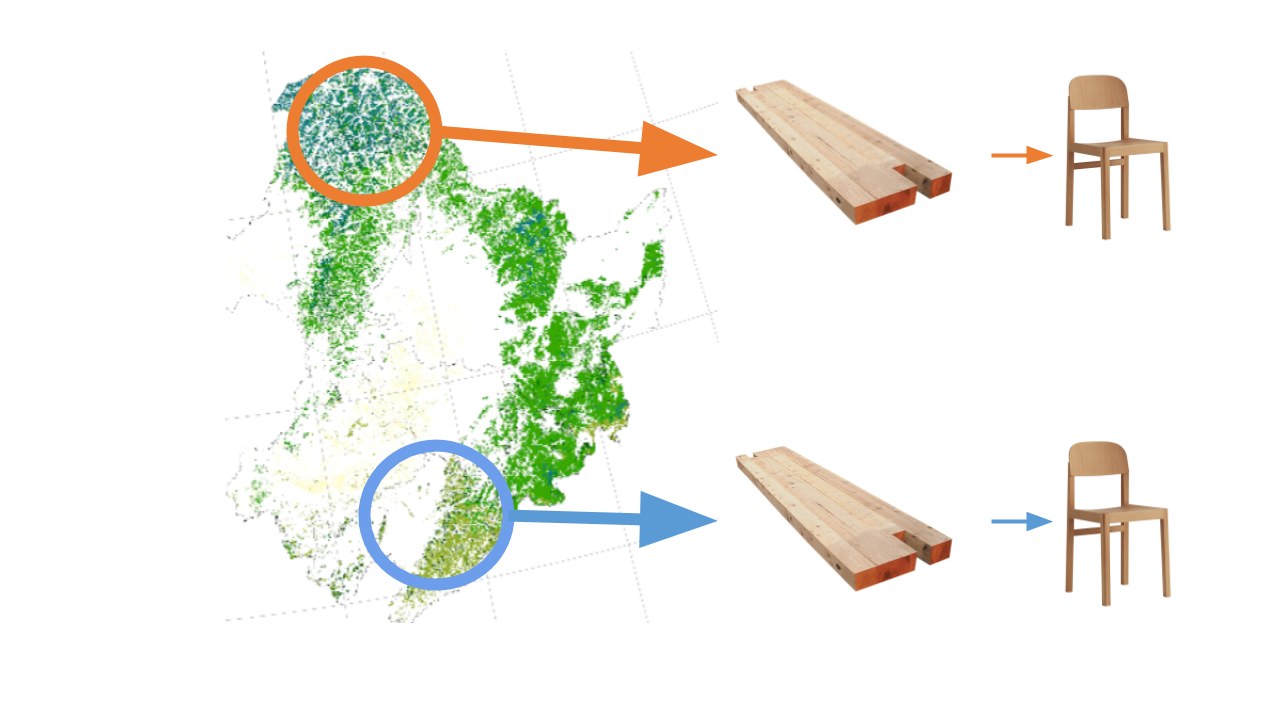
\includegraphics[keepaspectratio,
                              width=\paperwidth]{images/regionalize3.png}
            };
      \end{tikzpicture}
     \note[]{}
\end{frame}
}

{ %%% blank frame
\begin{frame}<article:0>[plain]
   \frametitle{}
      \begin{tikzpicture}[remember picture,overlay]
         \node[at=(current page.center)] {
             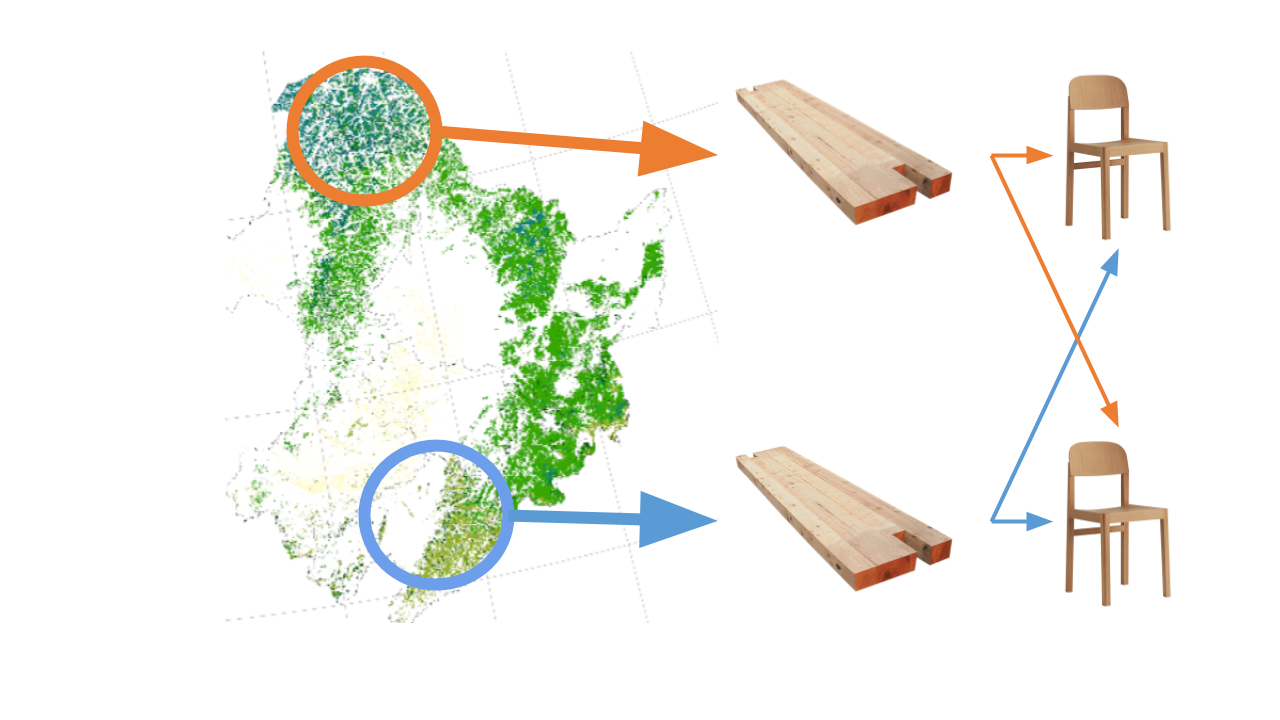
\includegraphics[keepaspectratio,
                              width=\paperwidth]{images/regionalize4.png}
            };
      \end{tikzpicture}
     \note[]{}
\end{frame}
}

{ 
\begin{frame}<article:0>[plain]
   \frametitle{}
      \begin{tikzpicture}[remember picture,overlay]
         \node[at=(current page.center)] {
             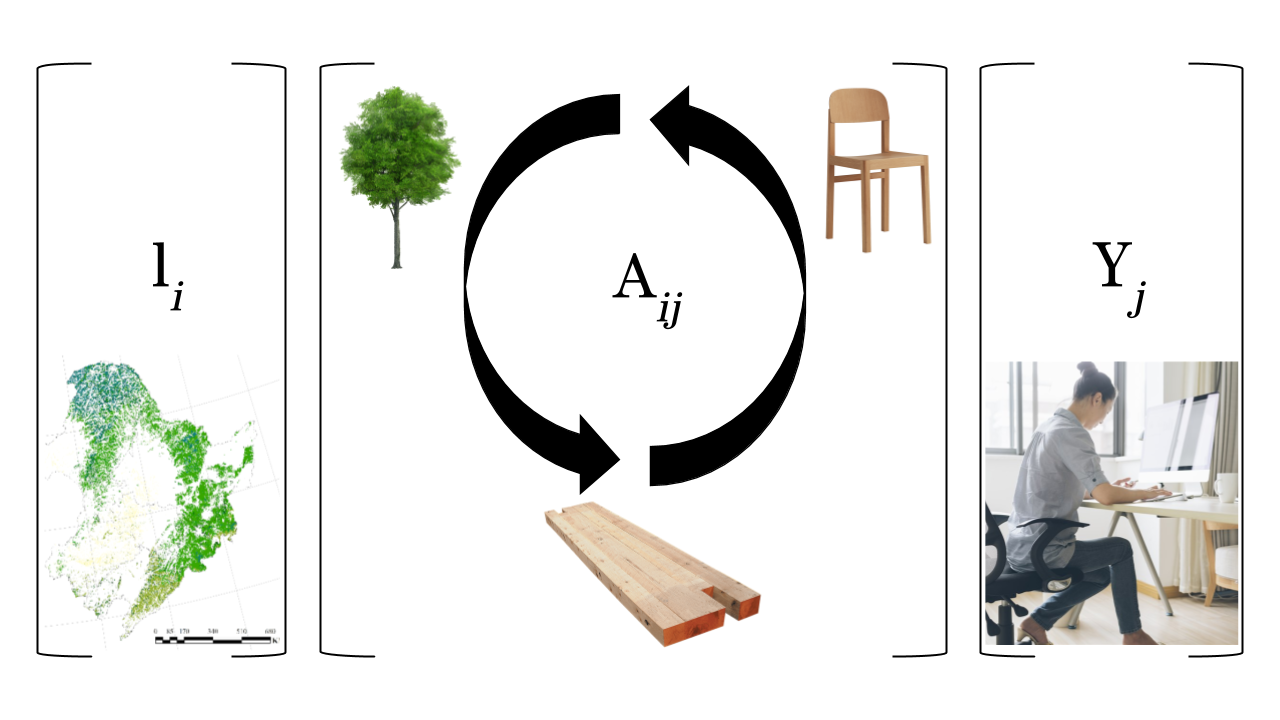
\includegraphics[keepaspectratio,
                              width=\paperwidth]{images/le-mrio-form.png}
            };
      \end{tikzpicture}
     \note[]{}
\end{frame}
}



{ 
\begin{frame}<article:0>[plain]
   \frametitle{}
      \begin{tikzpicture}[remember picture,overlay]
         \node[at=(current page.center)] {
             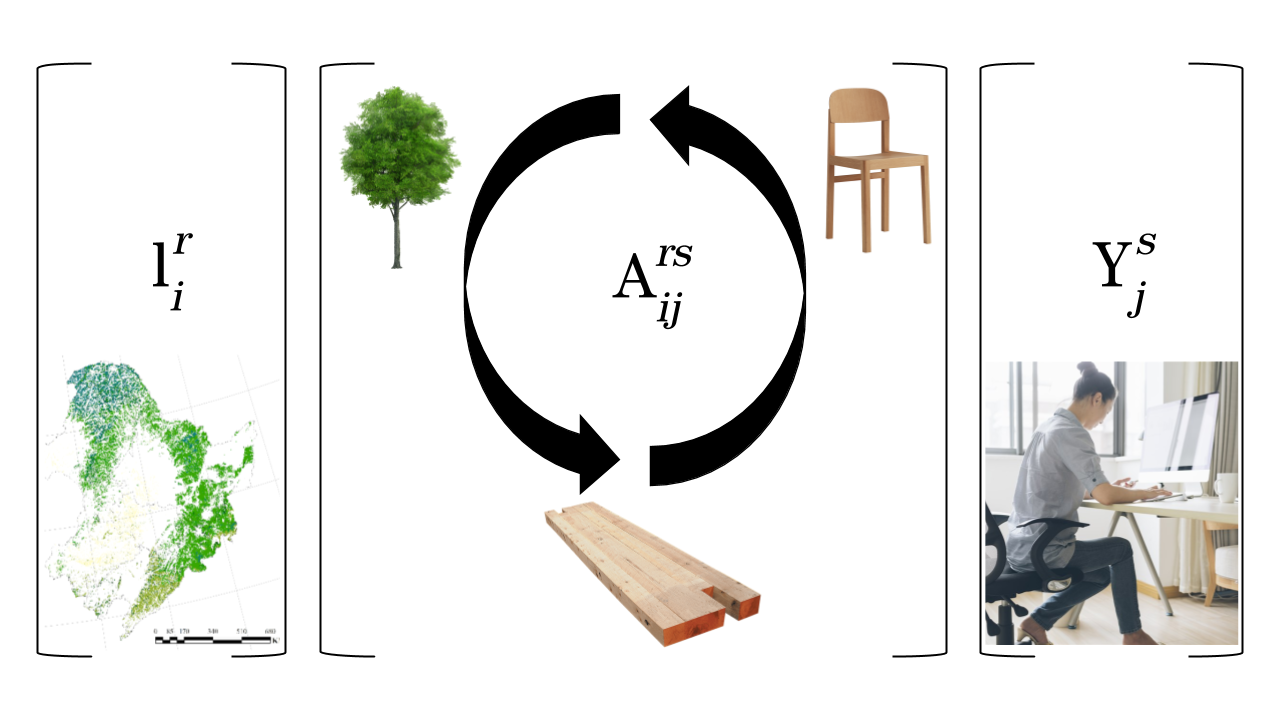
\includegraphics[keepaspectratio,
                              width=\paperwidth]{images/lemrio_rs.png}
            };
      \end{tikzpicture}
     \note[]{}
\end{frame}
}



{
\begin{frame}<article:0>[plain]
   \frametitle{}
      \begin{tikzpicture}[remember picture,overlay]
         \node[at=(current page.center)] {
             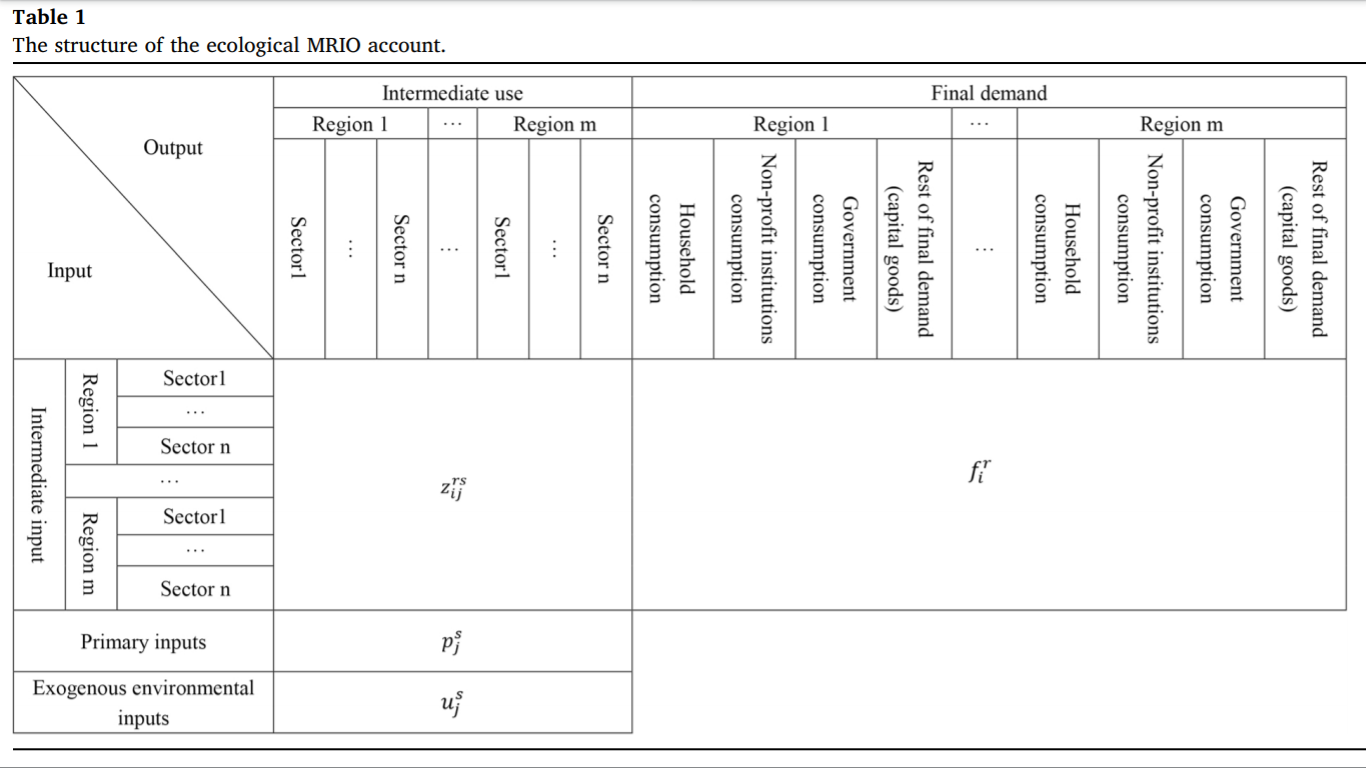
\includegraphics[keepaspectratio,
                              width=\paperwidth]{images/Wu_2018_Table1.png}
            };
      \end{tikzpicture}
     \note[item]{This is why they're called input-output tables}
     \note[item]{Each region has a set of sectors/industries}
     \note[item]{They can receive inputs from within a region}
     \note[item]{They can also receive input from another region (aka. imports)}
     \note[item]{Final use = Consumption not used to produce another product}
\end{frame}
}


\begin{frame}
  \frametitle{Environmental Extended Multi-Regional Input-Output Models}
  \begin{itemize}
  \item Many products are made from other products, so indirect use
  matters \pause
  \item Input-output modeling provides a framework to account for this \pause
  \item Environmental multipliers allow us to calculate ``embodied''
  ecological variables \pause
  \item Spatially explicit data allows us to regionalize our models \pause
    \end{itemize}
    \begin{center}
    \begin{equation}
        E_{j}^{s} = F_{i}^{r}(I - A_{ij}^{rs})^{-1}Y_{j}^{s}
    \end{equation}
    \end{center}
\end{frame}




\begin{frame}
  \frametitle{A few EE-MRIO Applications}
  \begin{itemize}
  \item Global carbon emissions are primarily indirect by developed
  country consumption (23\%) \cite{LIDDLE201871} \pause
  \item 17\% of biodiversity is embodied in food exported to
  high income countries \cite{CHAUDHARY2016195}  \pause
  \item Tropical forest loss in Brazil driven by conversion to soy
  exported primarily to China (48.6\%) and the USA (72.3\%) \cite{Schaffer-Smith2018}
  \end{itemize}
\end{frame}


%% { %%% blank frame
%% \begin{frame}<article:0>[plain]
%%    \frametitle{}
%%       \begin{tikzpicture}[remember picture,overlay]
%%          \node[at=(current page.center)] {
%%              \includegraphics[keepaspectratio,
%%                               width=\paperwidth]{images/}
%%             };
%%       \end{tikzpicture}
%%      \note[]{}
%% \end{frame}
%% }


\section{Global Trade Networks of Forest Landscapes}



\begin{frame}
  \frametitle{Global Embodied Landscape Trade Networks}
  \begin{itemize}
  \item What is the current state of forested landscapes \pause
  \item How does this relate to current patterns of landscape trade? \pause
  \item What is the role of China, which is a globally dominant
  economic consumer and producer?
  \end{itemize}
\end{frame}

{ 
\begin{frame}<article:0>[plain]
   \frametitle{}
      \begin{tikzpicture}[remember picture,overlay]
         \node[at=(current page.center)] {
             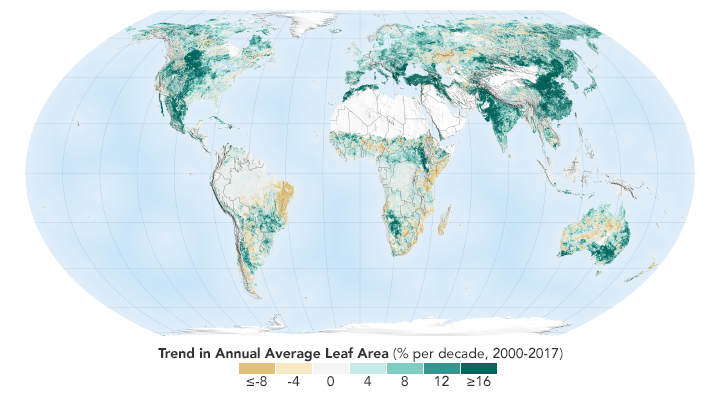
\includegraphics[keepaspectratio,
                              width=\paperwidth]{images/globalgreening_tamo_2017.png}
            };
      \end{tikzpicture}
     \note[item]{5\% increase in greening globally since 2000}
\end{frame}
}


{ 
\begin{frame}<article:0>[plain]
   \frametitle{}
      \begin{tikzpicture}[remember picture,overlay]
         \node[at=(current page.center)] {
             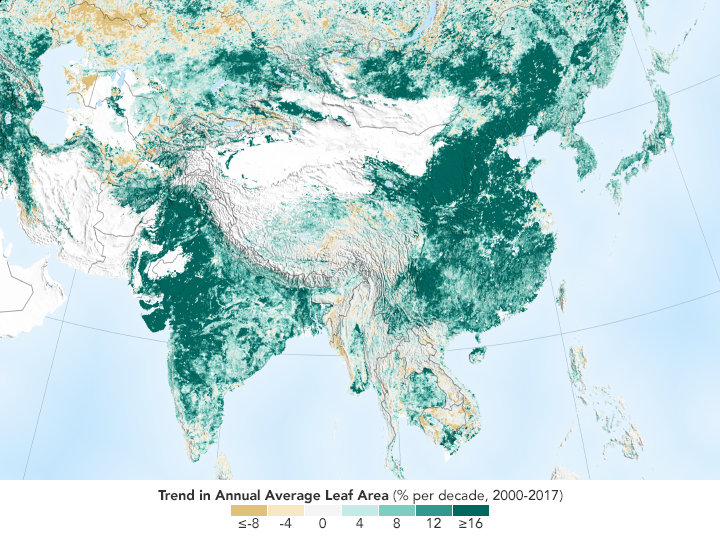
\includegraphics[keepaspectratio,
                              width=\paperwidth]{images/asia_greening_2017.png}
            };
      \end{tikzpicture}
     \note[item]{25\% from China}
     \note[item]{42\% from forest landscapes in China}
\end{frame}
}


{ 
\begin{frame}<article:0>[plain]
   \frametitle{}
      \begin{tikzpicture}[remember picture,overlay]
         \node[at=(current page.center)] {
             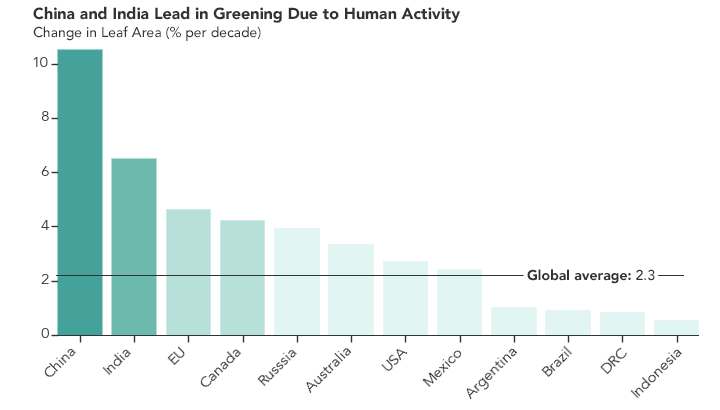
\includegraphics[keepaspectratio,
                              width=\paperwidth]{images/global_greening_2017.png}
            };
      \end{tikzpicture}
     \note[item]{China exceeds India by over 4\% of global green area}
     \note[item]{Increased plant, especially forest area is good, a
      positive outcome of human activities}
\end{frame}
}

{ % all template changes are local to this group.
%%    \setbeamertemplate{navigation symbols}{}
    \begin{frame}<article:0>[plain]
      \frametitle{}
        \begin{tikzpicture}[remember picture,overlay]
            \node[at=(current page.center)] {
                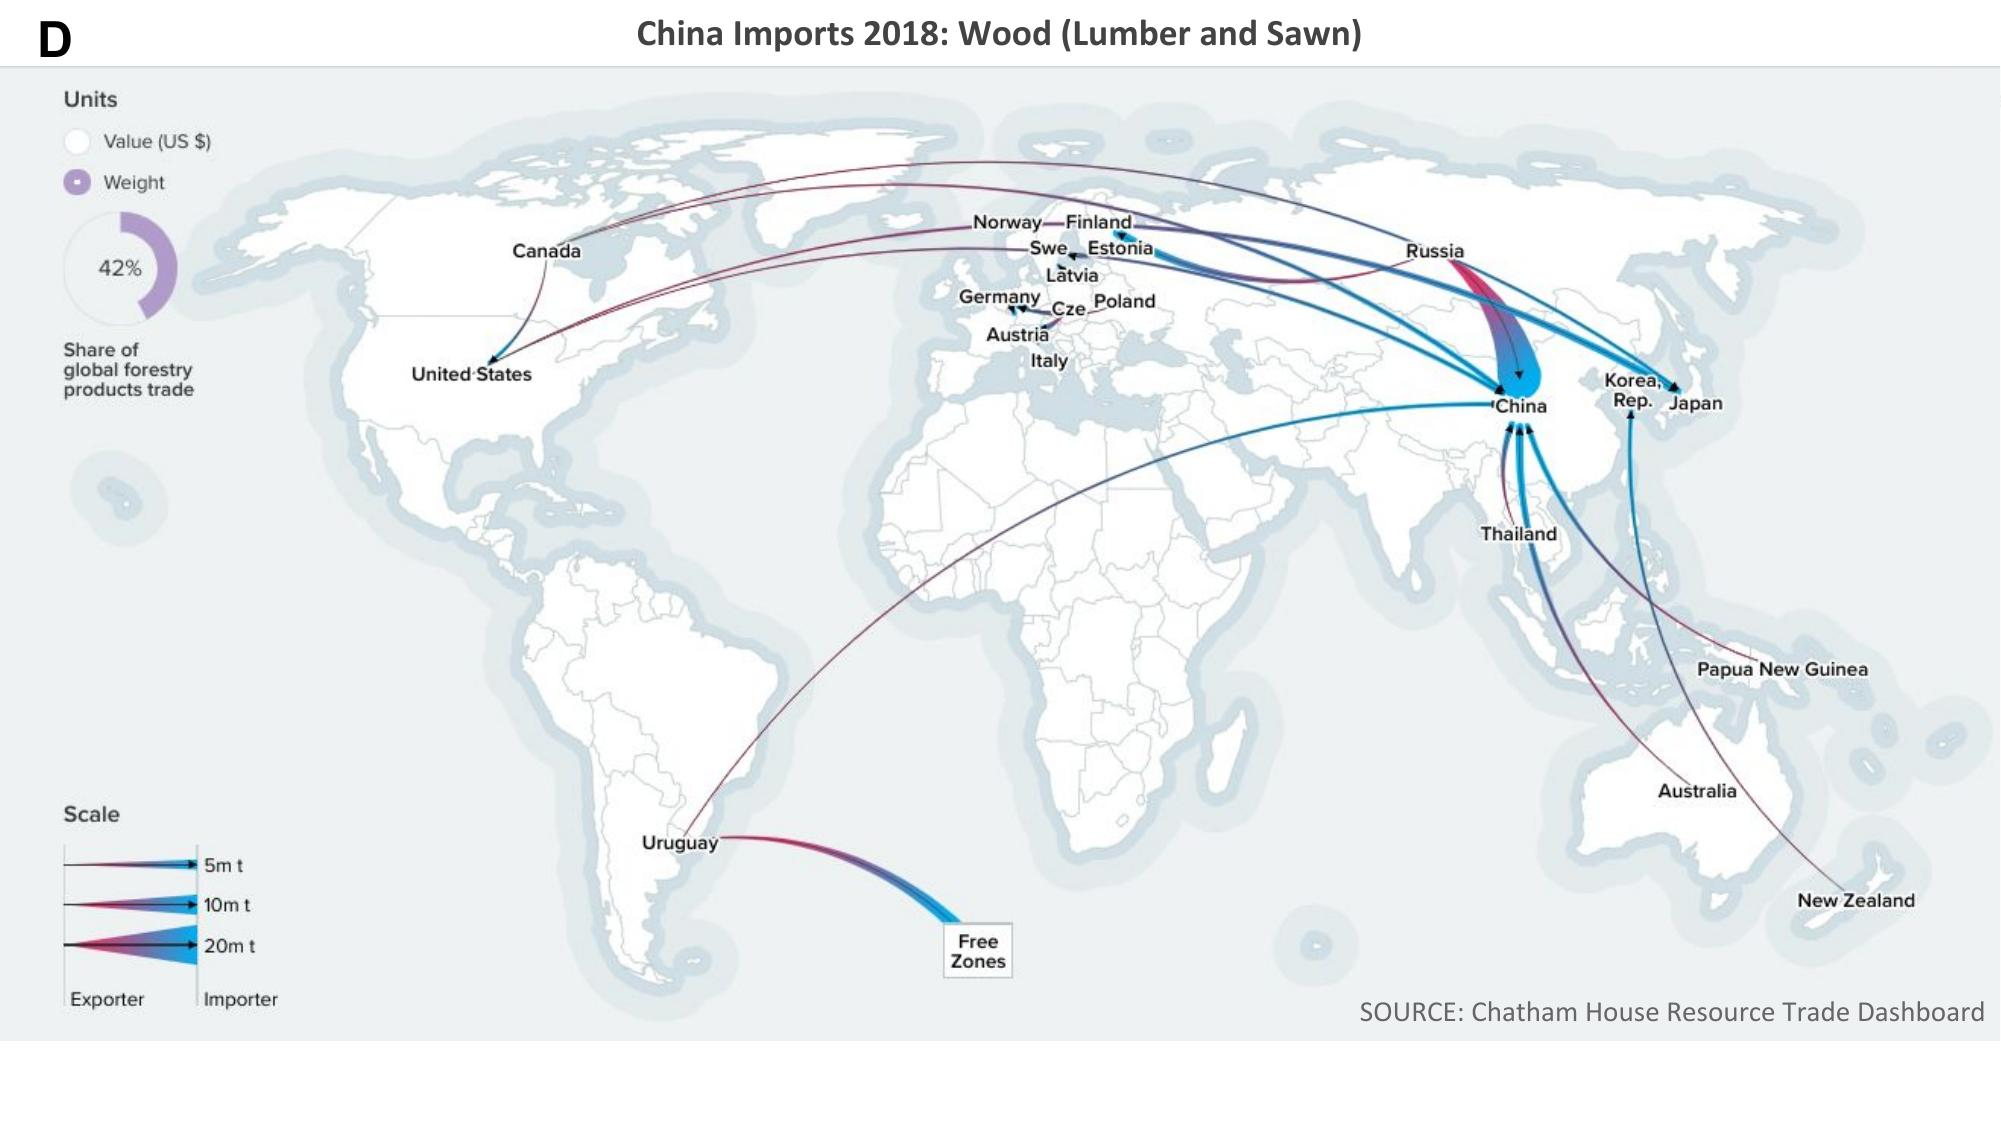
\includegraphics[keepaspectratio,
                                 width=\paperwidth]{images/resourcetrade_network.jpeg}
            };
        \end{tikzpicture}
     \note[item]{Considering trade in forest land, illustrates the
      importance of considering indirect effects in the Anthropocence}
     \end{frame}
}


\begin{frame}
  \frametitle{Global Embodied Landscape Trade Networks (Tian et al. 2019)}
    \begin{center}
    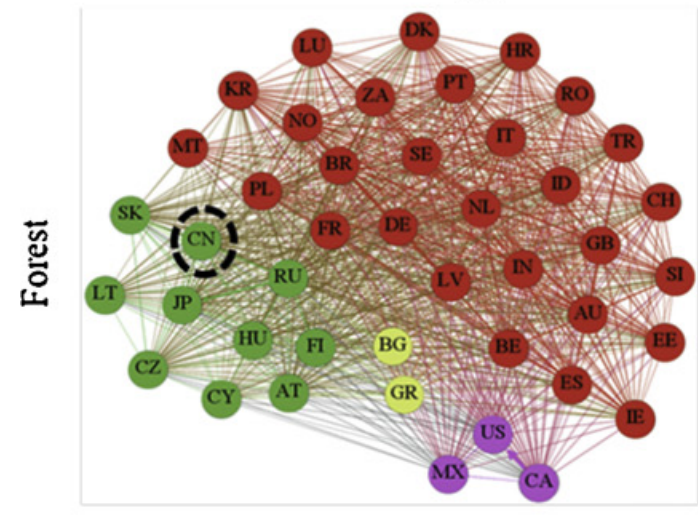
\includegraphics[width=0.5\textwidth]{images/Tian_2019_Fig3_inset_inset.png}  
    \end{center}
\end{frame}


\begin{frame}
  \frametitle{Global Embodied Landscape Trade Networks (Tian et al. 2019)}
  \begin{center}
  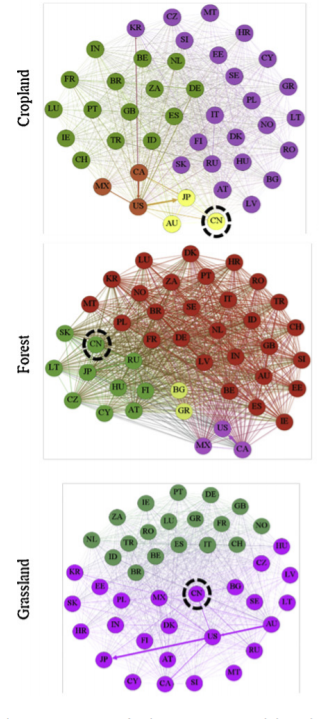
\includegraphics[width=0.2\textwidth]{images/Tian_2019_Fig3_inset.png}
  \end{center}
\end{frame}

\begin{frame}
  \frametitle{Global Embodied Landscape Trade Networks (Tian et al. 2019)}
  \begin{center}
  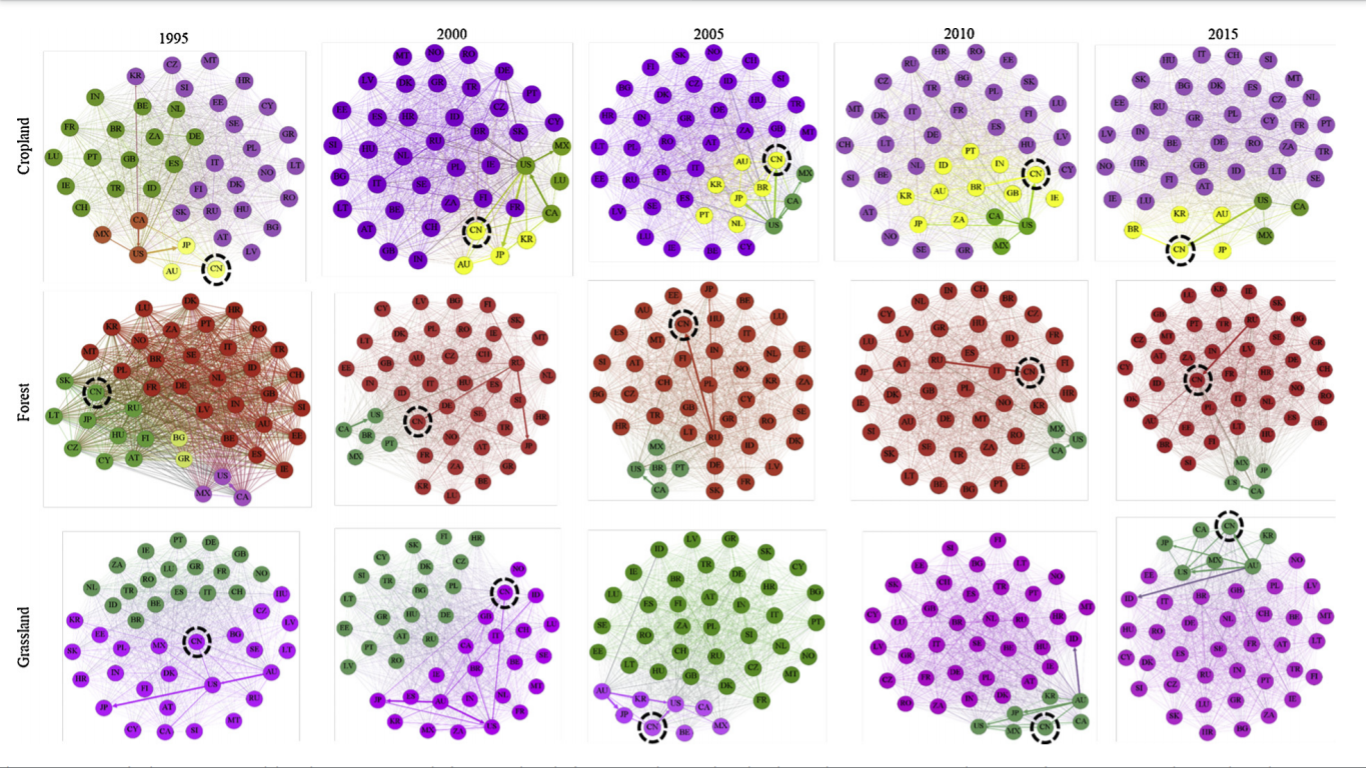
\includegraphics[width=0.95\textwidth]{images/Tian_2019_Fig3.png}
  \end{center}
\end{frame}




{ % all template changes are local to this group.
%%    \setbeamertemplate{navigation symbols}{}
    \begin{frame}<article:0>[plain]
      \frametitle{}
        \begin{tikzpicture}[remember picture,overlay]
            \node[at=(current page.center)] {
                \includegraphics[keepaspectratio,
                                 width=\paperwidth]{images/comtrade_china_imports_wood.jpeg}
            };
        \end{tikzpicture}
     \note[item]{China's imports have been increasing over time}
     \note[item]{Mostly from Russia and USA, lesser Canada and New Zealand}
     \note[item]{Cumulatively, southeast Asian countries rival Russia ($43,621)}
     \end{frame}
}

{ % all template changes are local to this group.
%%    \setbeamertemplate{navigation symbols}{}
    \begin{frame}<article:0>[plain]
      \frametitle{}
        \begin{tikzpicture}[remember picture,overlay]
            \node[at=(current page.center)] {
                \includegraphics[keepaspectratio,
                                 width=\paperwidth]{images/Tian_2019_Fig1.png}
            };
        \end{tikzpicture}
     \end{frame}
}

{ % all template changes are local to this group.
%%    \setbeamertemplate{navigation symbols}{}
    \begin{frame}<article:0>[plain]
      \frametitle{}
        \begin{tikzpicture}[remember picture,overlay]
            \node[at=(current page.center)] {
                \includegraphics[keepaspectratio,
                                 width=\paperwidth]{images/annual-change-forest-area.png}
            };
        \end{tikzpicture}
      \note[item]{Given China's importance in global forest dynamics,
      shocks to domestic consumption are important global as they can
      alter imports}
     \end{frame}
}



\begin{frame}
  \frametitle{Global Embodied Landscape Trade Networks}
  \begin{itemize}
  \item The Earth is getting greener, due in large part to forests in
  China \pause
  \item This greening is in part the result of national forest policy
  driven shifts in forest use \pause
  \item These shifts have concommitantly resulted in expansion of
  imports and deforestation through global trade networks \pause
  \item China is a dominant direct and indirect consumer of domestic
  and global forested lands
  \end{itemize}
\end{frame}


\section{China's Domestic Forest Land Network Structure}

\begin{frame}
     \frametitle{Network Structure of China's Domestic Forest Lands}
     \begin{center}
        \includegraphics[width=0.75\paperwidth]{images/le-mrio-form.png}
     \end{center}
     
\end{frame}


\begin{frame}
     \frametitle{Network Structure: Highly Localized Direct Use}
     \begin{center}
       \includegraphics[width=0.4\paperwidth]{images/heatmap_z_for.png}
     \end{center}
\end{frame}


\begin{frame}
     \frametitle{Network Structure: Three Modules}
     \begin{center}
        \includegraphics[width=0.75\paperwidth]{images/map_for_modularity.png}
     \end{center}
\end{frame}

\begin{frame}
     \frametitle{Network Structure: Dominated by Two Provinces}
     \begin{center}
        \includegraphics[width=0.75\paperwidth]{images/map_for_centrality.png}
     \end{center}
\end{frame}


\begin{frame}
     \frametitle{Network Structure to Dynamics}
     \begin{center}
        \includegraphics[width=0.5\paperwidth]{images/net_info_dynamics_inset.PNG}
     \end{center}
     
\end{frame}

\begin{frame}
     \frametitle{Network Structure to Dynamics}
     \begin{center}
        \includegraphics[width=0.5\paperwidth]{images/net_info_dynamics.PNG}
     \end{center}
     
\end{frame}



\begin{frame}
     \frametitle{Network Structure to Dynamics}
     \begin{center}
        \includegraphics[width=0.45\paperwidth]{images/for-rob-red.png}     
     \end{center}
\end{frame}


%% \begin{frame}
%%   \frametitle{Network Structure: Resilience(Efficiency, Redundancy)}
%%   \begin{center} 
%%    \begin{equation}
%%      H = -\sum_{i = 1}^{n} p_i ln(p_i)
%%   \end{center}
%% \end{frame}


%% \begin{frame}
%%   \frametitle{Network Structure: Resilience(Efficiency, Redundancy)}
%%   \begin{center} 
%%    \begin{equation}
%%     \Psi = -k\sum_{i=1,j=1}^{nn} \frac{T_{ij}}{T_{..}}\ln(\frac{T_{ij}^{2}}{T_{i.}T_{.j}})    \end{equation}
%%   \end{center}
%% \end{frame}


\section{Summary and Conclusions}


\begin{frame}
  \frametitle{Summary and Conclusions}
  \begin{itemize}
     \item The effects of the anthropocene has been globalization of
     economies and de-stabiliziation of the environment \pause
     \item China is a driver of forest dynamics globally with
  increasing imports of forested landscapes from foreign countries \pause
     \item China's domestic forest landscape network structure is
  highly modular relative to provincial industries and nationally
  modular at a broad regional scale (north, south and west) \pause
     \item The provincial industries that rely on forest landscapes
  are potentially sub-optimally structured relative to food-webs \pause
  \item \textbf{Take-Home}: structural analysis of global and domestic
  networks provide a necessary insight into human impacts on Earth,
  suggesting the need/opportunity for international coordination in
  environmental issues.
\end{itemize}
\end{frame}


\section{Future Work}

\begin{frame}
  \frametitle{Future Work: CAS Grant (2021-2023)}
\begin{columns}
\begin{column}{0.5\textwidth}
    \begin{center}
     \includegraphics[width=0.86\textwidth]{images/moran_2020_1.png}
     \end{center}
\end{column}
\begin{column}{0.5\textwidth}  %%<--- here
    \begin{center}
     \includegraphics[width=1.0\textwidth]{images/moran_2020_2.png}
     \end{center}
\end{column}
\end{columns}
\end{frame}

\begin{frame}
  \frametitle{Future Work: CAS Grant (2021-2023)}
    \begin{center}
     \includegraphics[width=1.0\textwidth]{images/lemrio_climate_change.jpeg}
     \end{center}
\end{frame}


\begin{frame}
  \frametitle{Cool Projects to Check Out}
  \begin{itemize}
  \item \url{www.globalcanopy.org} - Financial Sector Transparency
  \item \url{www.fineprint.global} - Product Sourcing Analysis 
  \item \url{trase.earth} - Stakeholder and Investor Information
  \end{itemize}
\end{frame}


\begin{frame}
  \frametitle{Acknowledgements}
\end{frame}

{ % all template changes are local to this group.
%%    \setbeamertemplate{navigation symbols}{}
    \begin{frame}<article:0>[plain]
      \frametitle{}
        \begin{tikzpicture}[remember picture,overlay]
            \node[at=(current page.center)] {
                \includegraphics[keepaspectratio,
                                 width=\paperwidth]{images/cn_for_yu/IMG_0233.JPG}
            };
        \end{tikzpicture}
        \note[item]{Funding from the CAS PIFI program}
        \note[item]{Institutional support and compute resources from
      Harvard University and Harvard Forest}
        \note[item]{Thanks to all of the folks in the LSP Lab for
      providing help with aquiring data for the project and conceptul
      development}
        \note[item]{Particularly Dr Yu Liang who heads the lab for
      hosting me during my stay and travels in China}
     \end{frame}
}

{ % all template changes are local to this group.
%%    \setbeamertemplate{navigation symbols}{}
    \begin{frame}<article:0>[plain]
      \frametitle{}
        \begin{tikzpicture}[remember picture,overlay]
            \node[at=(current page.center)] {
                \includegraphics[keepaspectratio,
                                 width=\paperwidth]{images/cn_for_yu/IMG_0240.JPG}
            };
        \end{tikzpicture}
        \note[item]{Questions, comments?}
        \note[item]{I'll provide my slides with notes}
     \end{frame}
}




\begin{frame}[allowframebreaks]
  \frametitle{References}
  \tiny \bibliography{biblio.bib}
  \bibliographystyle{abbrv}
\end{frame}


{
\usebackgroundtemplate{
\begin{tikzpicture}[remember picture,overlay]
        \node[at=(current page.center), opacity=0.40]{
                \includegraphics[keepaspectractio, width=\paperwidth]{images/forest_aerial.jpg}
        };
\end{tikzpicture}
}
\begin{frame}
  \titlepage
  \note[item]{Thanks to Dave Smith and anyone else who's helped to
  organize this seminar, it's a pleasure for me to speak about my
  recent work}
  \note[item]{Forests $\sim$ 80\% terrestrial biodiversity (WWF)}
  \note[item]{Soil stabilization}
  \note[item]{Forests carry out important processes: clean air and water}
  \note[item]{Forests store carbon}
\end{frame}
}


\end{document}

